\documentclass[
	12pt,
	a4paper,
	bibtotoc,
	cleardoubleempty, 
	idxtotoc,
	ngerman,
	openright
	final,
	listof=nochaptergap,
	]{scrbook}
\usepackage{cmap}
\usepackage[T1]{fontenc}
\usepackage[utf8]{inputenc}
\usepackage{pdfpages}
\usepackage{nameref}
\usepackage{dirtytalk}
\usepackage{natbib}

% ##################################################
% Unterstuetzung fuer die deutsche Sprache
% ##################################################
%\usepackage{ngerman}
\usepackage[ngerman]{babel}
\usepackage{graphicx}
\usepackage{wrapfig}

% ##################################################
% Dokumentvariablen
% ##################################################

% Persoenliche Daten
\newcommand{\docNachname}{Häcker}
\newcommand{\docVorname}{Nick Philipp}
\newcommand{\docStrasse}{Gaußstraße 82a}
\newcommand{\docOrt}{Stuttgart}
\newcommand{\docPlz}{70193}
\newcommand{\docEmail}{nick.athaeck@gmail.com}
\newcommand{\docMatrikelnummer}{274095}

% Dokumentdaten
\newcommand{\docTitle}{Konzeption und Entwicklung einer asymmetrischen AR-/3D-Multiplayer-Anwendung zur Beobachtung des Kommunikationsverhaltens zwischen Individuen}
%\newcommand{\docUntertitle}{} % Kein Untertitel
\newcommand{\docUntertitle}{Connecting-Minds}
% Arten der Arbeit: Bachelorthesis, Masterthesis, Seminararbeit, Diplomarbeit
\newcommand{\docArtDerArbeit}{Thesis zum Erlangen des Grades Master of Science}
%Studiengaenge: Allgemeine Informatik Bachelor, Computer Networking Bachelor,
% Software-Produktmanagement Bachelor, Advanced Computer Scinece Master
\newcommand{\docStudiengang}{Medieninformatik (MIM)}
\newcommand{\docAbgabedatum}{Endabgabe eingeben}
\newcommand{\docErsterReferent}{Prof. Dr. Thomas Schlegel}
%\newcommand{\docZweiterReferent}{-} % Wenn es nur einen Betreuer gibt
\newcommand{\docZweiterReferent}{Prof. Jirka Dell´Oro-Friedl}

% ##################################################
% Allgemeine Pakete
% ##################################################

% Abbildungen einbinden
\usepackage{graphicx}

% Zusaetsliche Sonderzeichen
\usepackage{dingbat}

% Symbole Haken und X [OPTIONAL]
%\usepackage{pifont}
%\newcommand{\cmark}{\ding{51}}
%\newcommand{\xmark}{\ding{55}}

% Farben
\usepackage{color}
\usepackage[usenames,dvipsnames,svgnames,table]{xcolor}

% Maskierung von URLs und Dateipfaden
\usepackage[hyphens]{url}

% Deutsche Anfuehrungszeichen
\usepackage[babel, german=quotes]{csquotes}

% Pakte zur Index-Erstellung (Schlagwortverzeichnis)
\usepackage{index}
\makeindex

% Ipsum Lorem
% Paket wird nur für das Beispiel gebraucht und kann gelöscht werden
\usepackage{lipsum}

% ##################################################
% Seitenformatierung
% ##################################################
\usepackage[
	portrait,
	bindingoffset=1.5cm,
	inner=2.5cm,
	outer=2.5cm,
	top=3cm,
	bottom=2cm,
	%showframe, %Aktivieren um Seitengrenzen anzuzeigen
	%includeheadfoot
	]{geometry}

% ##################################################
% Kopf- und Fusszeile
% ##################################################

\usepackage{fancyhdr}

\pagestyle{fancy}
\fancyhf{}
\fancyhead[EL,OR]{\sffamily\thepage}
\fancyhead[ER,OL]{\sffamily\nouppercase{\leftmark}}

\fancypagestyle{headings}{}

\fancypagestyle{plain}{}

\fancypagestyle{empty}{
  \fancyhf{}
  \renewcommand{\headrulewidth}{0pt}
}

%Speichert \chaptermark in \oldchaptermark damit 
% es für die Anhänge zurückgesetzt werden kann
\let\oldchaptermark\chaptermark

%Kein "Kapitel # NAME" in der Kopfzeile
\renewcommand{\chaptermark}[1]{
	\markboth{#1}{}
   	\markboth{\thechapter.\ #1}{}
}

% ##################################################
% Schriften
% ##################################################

% Stdandardschrift festlegen
\renewcommand{\familydefault}{\sfdefault}

% Standard Zeilenabstand: 1,5 zeilig
\usepackage{setspace}
\onehalfspacing 

% Schriftgroessen festlegen
\addtokomafont{chapter}{\sffamily\large\bfseries} 
\addtokomafont{section}{\sffamily\normalsize\bfseries} 
\addtokomafont{subsection}{\sffamily\normalsize\mdseries} 
\addtokomafont{caption}{\sffamily\normalsize\mdseries} 

%Einrücken von Absätzen deaktivieren
\setlength{\parindent}{0pt}

%Zeilenabstand bei abstätzen
\usepackage{parskip}

% ##################################################
% Inhaltsverzeichnis / Allgemeine Verzeichniseinstellungen
% ##################################################

\usepackage{tocloft}

% Punkte auch bei Kapiteln
\renewcommand{\cftchapdotsep}{3}
\renewcommand{\cftdotsep}{3}

% Schriftart und -groesse im Inhaltsverzeichnis anpassen
\renewcommand{\cftchapfont}{\sffamily\normalsize}
\renewcommand{\cftsecfont}{\sffamily\normalsize}
\renewcommand{\cftsubsecfont}{\sffamily\normalsize}
\renewcommand{\cftchappagefont}{\sffamily\normalsize}
\renewcommand{\cftsecpagefont}{\sffamily\normalsize}
\renewcommand{\cftsubsecpagefont}{\sffamily\normalsize}

%Zeilenabstand in den Verzeichnissen einstellen
\setlength{\cftparskip}{.5\baselineskip}
\setlength{\cftbeforechapskip}{.1\baselineskip}

%Einrücken von Absätzen deaktivieren
%\setlength{\parindent}{0pt}

%Zeilenabstand bei abstätzen
\usepackage{parskip}

% ##################################################
% Abbildungsverzeichnis und Abbildungen
% ##################################################

\usepackage{caption}

\usepackage{wrapfig}

% Nummerierung von Abbildungen
\renewcommand{\thefigure}{\arabic{figure}}
\usepackage{chngcntr}
\counterwithout{figure}{chapter}

% Abbildungsverzeichnis anpassen
\renewcommand{\cftfigpresnum}{Abbildung }
\renewcommand{\cftfigaftersnum}{:}

% Breite des Nummerierungsbereiches [Abbildung 1:]
\newlength{\figureLength}
\settowidth{\figureLength}{\bfseries\cftfigpresnum\cftfigaftersnum}
\addtolength{\figureLength}{2mm} %extra offset
\setlength{\cftfignumwidth}{\figureLength}
\setlength{\cftfigindent}{0cm}

% Schriftart anpassen
\renewcommand\cftfigfont{\sffamily}
\renewcommand\cftfigpagefont{\sffamily}

%standardpfad anpassen
\graphicspath{ {../src/content/pictures/} }

% ##################################################
% Tabellenverzeichnis und Tabellen
% ##################################################

% Nummerierung von Tabellen
\renewcommand{\thetable}{\arabic{table}}
\counterwithout{table}{chapter}

% Tabellenverzeichnis anpassen
\renewcommand{\cfttabpresnum}{Tabelle }
\renewcommand{\cfttabaftersnum}{:}

% Breite des Nummerierungsbereiches [Abbildung 1:]
\newlength{\tableLength}
\settowidth{\tableLength}{\bfseries\cfttabpresnum\cfttabaftersnum}
\addtolength{\tableLength}{3mm} %extra offset
\setlength{\cfttabnumwidth}{\tableLength}
\setlength{\cfttabindent}{0cm}

%Schriftart anpassen
\renewcommand\cfttabfont{\sffamily}
\renewcommand\cfttabpagefont{\sffamily}

% Unterdrueckung von vertikalen Linien
\usepackage{booktabs}

%Multi row für spezifische zellen
\usepackage{multirow}

%Additional table package
\usepackage{tabu}

% ##################################################
% Listings (Quellcode)
% ##################################################

\usepackage{listings}

%use typewriter font which supports bold characters
\usepackage{beramono}

\definecolor{codegreen}{rgb}{0,0.6,0}
\definecolor{codegray}{rgb}{0.5,0.5,0.5}
\definecolor{codepurple}{rgb}{0.5,0,0.33}
\definecolor{codepurblue}{rgb}{0.16,0.0,1.0}
\definecolor{backcolour}{rgb}{0.95,0.95,0.92}

\lstdefinestyle{codestyle}{
    backgroundcolor=\color{backcolour},   
    commentstyle=\color{codegreen},
    keywordstyle=\bfseries\color{codepurple},
    numberstyle=\tiny\color{codegray},
    stringstyle=\color{codepurblue},
    basicstyle=\scriptsize\ttfamily,
    breakatwhitespace=false,         
    breaklines=true,                 
    captionpos=b,                    
    keepspaces=true,                 
    numbers=left,                     
    numbersep=5pt,                 
    showspaces=false,                
    showstringspaces=false,
    showtabs=false,                  
    tabsize=2
}

\lstset{style=codestyle}

%Code auschnitt importieren aus datei
%\mylisting{from}{to}{language}{file}{descr}{path}
\newcommand{\mylisting}[6]{
\lstinputlisting[language=#3,
				firstnumber=#1,
				firstline=#1,
				lastline=#2,
				caption={#4, #5}, 
				label={implementation_listing_#4_#5}]
				{#6}
}

% ##################################################
% Appendix
% ##################################################

%Calc packet für berechnungen
\usepackage{calc}

%Appendix paket, setzen der flags für das TOC
\usepackage[toc,title,titletoc]{appendix} 

%Umbenennen der überschrift für die Anhänge 
\renewcommand{\appendixtocname}{Anhänge}

%Befehl für einen neuen Bericht und die erste seite als bild
\newcommand{\appendixsection}[2]{
\section{#1}
\appendixsingle{#2}
}

%Befehl für einzelne seite als bild eingefasst, damit überschrift und kopfzeile
% bestehen bleibt. 
\newcommand{\appendixsingle}[1]{
\vspace{-10cm}
\vfill
\mbox{}\hspace{-1.5cm}\includegraphics[width=\linewidth+3cm]{#1}\hspace{-1.5cm}\mbox{}
\vspace{-10cm}
\vfill
\mbox{}
}

%Datenträger Tabelle
\definecolor{lightgray}{gray}{0.85}
\definecolor{ultralightgray}{gray}{0.95}
\definecolor{mygray}{gray}{0.70}

% ##################################################
% Theoreme
% ##################################################
  	
% Umgebung fuer Beispiele
\newtheorem{beispiel}{Beispiel}

% Umgebung fuer These
\newtheorem{these}{These}

% Umgebung fuer Definitionen
\newtheorem{definition}{Definition}
  	
% ##################################################
% Literaturverzeichnis
% ##################################################

\usepackage{bibgerm}

% ##################################################
% Abkuerzungsverzeichnis
% ##################################################

\usepackage[printonlyused]{acronym}

% ##################################################
% PDF / Dokumenteninternelinks
% ##################################################

\usepackage[
	colorlinks=false,
   	linkcolor=black,
   	citecolor=black,
  	filecolor=black,
	urlcolor=black,
    bookmarks=true,
    bookmarksopen=true,
    bookmarksopenlevel=3,
    bookmarksnumbered,
    plainpages=false,
    pdfpagelabels=true,
    hyperfootnotes,
    pdftitle ={\docTitle},
    pdfauthor={\docVorname~\docNachname},
    pdfcreator={\docVorname~\docNachname}]{hyperref}
    \hypersetup{
    colorlinks,
    citecolor=black,
    filecolor=black,
    linkcolor=black,
    urlcolor=black
}

% ####################################################
% Command für einfache QUellenangabe bei Bilder, etc.
% ####################################################

\newcommand{\source}[1]{\caption*{Quelle: {#1}} }


\begin{document}

\setcounter{secnumdepth}{3}

% Titelblatt
\begin{titlepage}
\pagestyle{empty}

% ##################################################
% HFU-Logo einbinden
% ##################################################
\begin{flushright}
\begin{figure}[ht]
\flushright

\includegraphics[height=3cm]{content/pictures/hfu.jpg}
\end{figure}
\end{flushright}

% ##################################################
% Titel
% ##################################################
\begin{center}
{\fontsize{18}{22} \selectfont \docArtDerArbeit}\\[5mm]
{\fontsize{18}{22} \selectfont im Studiengang} \\[5mm]
{\fontsize{18}{22} \selectfont \docStudiengang}\\
\vspace{1cm}
\begin{onehalfspace}
{\fontsize{22}{26} \selectfont \textbf{\docTitle}}\\[5mm]
% {\fontsize{18}{22} \selectfont \docUntertitle}


\end{onehalfspace}
\end{center}

% ##################################################
% Zusatzinformationen
% ##################################################
\vfill
\begin{center}
\begin{tabular}{lcl}
Erstbetreuer  		&:& \docErsterReferent 	\\ \\
Zweitbetreuer 		&:& \docZweiterReferent \\ \\	
Vorgelegt am 	&:& \docAbgabedatum 	\\ \\
Vorgelegt von 	&:& \docVorname~\docNachname\\
				& & Matrikelnummer: \docMatrikelnummer\\
				& & \docStrasse,~\docPlz~\docOrt	\\
				& & \docEmail			
\end{tabular}
\end{center}
\end{titlepage}
\cleardoubleemptypage

\frontmatter
\pagenumbering{Roman}

% Abstract
\chapter*{Abstract\markboth{Abstract}{}}
\addcontentsline{toc}{chapter}{Abstract}



% [TODO: Zusammenfassung der Arbeit schreiben]
% \say{\emph{A Fraction of Time}} basiert auf der Idee, den Spieler verschiedene parallele Zeitlinien von sich selbst erzeugen zu lassen. Der Spieler muss in diesen verschiedenen Zeitlinien, mithilfe der diversen Zeitlinien von sich selbst, Rätsel lösen und mit seinen Zeitlinien zusammenarbeiten. Grundlage dieser Weiterentwicklung ist der digitale Prototyp, der bereits im Gamedesign Workshop im Wintersemester 2021/ 2022 entwickelt wurde. 

% Die Zielsetzung dieser Abschlussarbeit ist es, das bisher implementierte System auf technischer Seite soweit zu verbessern, dass es für den Spieler offensichtlich fehlerfrei funktioniert. Außerdem soll ein Rahmen geschaffen werden, in dem es möglich ist, Erweiterungen zu integrieren. Hinzu werden weitere Inhalte, wie weitere Level und Spielwelten konzipiert und umgesetzt. Der Spieler soll dabei eine Variation an Spielwelten und Rätsel erhalten, welche er lösen muss, um das Level abzuschließen. Hierbei soll ihm auch das Spielprinzip so vermittelt werden, dass er durch das Verständnis der Mechanik jedes Rätsel lösen kann. Validiert werden die Inhalte durch User-Tests, bei denen das Verständnis der Spielmechanik auf inhaltlicher und technischer Ebene abgefragt wird.
\cleardoubleemptypage

\chapter*{Gender-Hinweis\markboth{Gender-Hinweis}{}}
\addcontentsline{toc}{chapter}{Gender-Hinweis}

Zur besseren Lesbarkeit wird in dieser Hausarbeit das generische Maskulinum verwendet. Die in dieser Arbeit verwendeten Personenbezeichnungen beziehen sich – sofern nicht anders kenntlich gemacht – auf alle Geschlechter.
\cleardoubleemptypage

% Inhaltsverzeichnis
\phantomsection
\addcontentsline{toc}{chapter}{Inhaltsverzeichnis}
\tableofcontents
\cleardoubleemptypage

% Abbildungsverzeichnis einbinden und ins Inhaltsverzeichnis
% WORKAROUND: tocloft und KOMA funktionieren zusammen nicht
% korrekt\phantomsection
\phantomsection 
\addcontentsline{toc}{chapter}{\listfigurename} 
\listoffigures
\cleardoubleemptypage

% Tabellenverzeichnis einbinden und ins Inhaltsverzeichnis
% WORKAROUND: tocloft und KOMA funktionieren zusammen nicht
% korrekt\phantomsection
\phantomsection
\addcontentsline{toc}{chapter}{\listtablename}
\listoftables
\cleardoubleemptypage

% Quellcodeverzeichnis einbinden und ins Inhaltsverzeichnis
\phantomsection
\addcontentsline{toc}{chapter}{Quellcodeverzeichnis}

%Define listing
\makeatletter
\begingroup\let\newcounter\@gobble\let\setcounter\@gobbletwo
  \globaldefs\@ne \let\c@loldepth\@ne
  \newlistof{listings}{lol}{\lstlistlistingname}
\endgroup
\let\l@lstlisting\l@listings
\makeatother
\setlength{\cftlistingsindent}{0em}
\renewcommand{\cftlistingsafterpnum}{\vskip0pt} %Spacing between entries
\renewcommand*{\cftlistingspresnum}{\lstlistingname~}
\settowidth{\cftlistingsnumwidth}{\cftlistingspresnum}
\renewcommand{\lstlistlistingname}{Quellcodeverzeichnis}
% Tabellenverzeichnis anpassen
\renewcommand{\lstlistingname}{Codeauschnitt}
\renewcommand{\cftlistingsaftersnum}{:}
% Breite des Nummerierungsbereiches [Codeauschnitt 1:]
\newlength{\codeLength}
\settowidth{\codeLength}{\bfseries\lstlistingname\cftlistingsaftersnum}
\addtolength{\codeLength}{5mm}
\setlength{\cftlistingsnumwidth}{\codeLength}
\lstlistoflistings
\cleardoubleemptypage

% Abkürzungsverzeichnis
\chapter*{Abkürzungsverzeichnis\markboth{Abkürzungsverzeichnis}{}}
\addcontentsline{toc}{chapter}{Abkürzungsverzeichnis}

\begin{acronym}
\acro{HFU}{Hochschule Furtwangen University}
\acro{DIM}{Design Interaktiver Medien}
\acro{MIM}{Medieninformatik Master}
\acro{MUD}{Multi-User-Dungeon}
\acro{MBTI}{Myer-Briggs Type Indicator}
\acro{UCD}{User Centered Design}
\acro{P2P}{Peer-to-Peer}
\acro{CSCW}{Conference on Computer-Supported Cooperative Work \& Social Computing}
\acro{HCI}{Human-Computer Interaction}
\acro{CHI}{Conference on Human Factors in Computing Systems}
\acro{MMOG}{Massively Multiplayer Online Game}
\acro{VR}{Virtual Reality}
\acro{AR}{Augmented Reality}
\acro{MR}{Mixed-Reality}
\acro{RPG}{Role Playing Game}
\acro{MDA}{Mechanics, Dynamics and Aesthetics}
\acro{Sci-Fi}{Science-Fiction}
\acro{UI}{User Interface}
\acro{MVP}{Minimum Viable Product}
\acro{MVC}{Model-View-Controller}
\acro{CMP}{Cooperative Performance Metrics}
\acro{RTS}{Real-Time-Strategy}
\acro{LTS}{Long-Term-Support}
\acro{FBX}{Filebox}
\acro{OBJ}{Object}
\acro{AI}{Artificial Intelligence}
\acro{URP}{Universal Render Pipeline}
\acro{3D}{dreidimensional}
\acro{URL}{Uniform Resource Locator}
\acro{NPM}{Node Package Manager}
\acro{HUD}{Head-up-Display}
\acro{OSI}{Open Systems Interconnection}
\acro{UDP}{User Datagram Protocol}
\acro{TCP}{Transmission Control Protocol}
\acro{SYN}{Synchronize}
\acro{ACK}{Acknowledgement}
\acro{HTTP}{Hypertext Transfer Protocol}
\acro{IT}{Information Technology}
\acro{IIIUS}{Institut für Intelligente Interaktive Ubiquitäre Systeme}
\acro{SUS}{System Usability Scale}
\acro{IEQ}{Immersive Experience Questionnaire}
\acro{GEQ}{Game Experience Questionnaire}
\acro{NASA-TLX}{NASA Task Load Index}
\acro{SAM}{Self-Assessment Manikin}
\acro{IOS}{Inclusion of the Other in the Self}
\acro{IMI}{Intrinsic Motivation Inventory}
\acro{M}{Mittelwert}
\acro{SD}{Standardabweichung}
\acro{Q-Q}{Quantil-Quantil}
\acro{CF}{Collaborative Floor Holding}
\acro{SF}{Single Floor Holding}
\acro{VE}{Virtual Environments}
\acro{HMD}{Head-Mounted-Display}
\acro{XR}{Extended Reality}
\acro{VC}{Virtuality Continuum}
\acro{AV}{Augmented Virtuality}
\acro{PR}{Physcial Reality}
\acro{HAR}{Handheld Augmented Reality}
\acro{SAR}{Spatial Augmented Reality}
\end{acronym}

\mainmatter

\chapter{Einleitung}
% Einleitung über Themen von multiplayern, zusammen spielen, vl corona noch, dann darüber dass es wenig asymmetrische multiplayer gibt, irgendwie steam lib durchgehen oder andere Listen noch, verweise auf crossplattform noch geben da es ähnlich wäre.

% Einsamkeitsstudien von corona zeigen und auflisten von studien or Papern bei denen es darum geht, dass die Spiele spaßig sind und kommunikationsfördernd und social engagement steigernd sind um sowas wie corona entgegenzuwirken.

% Kurzer Überblick über den Beginn der Arbeit; enthält den Interaktionsdesignworkshop
% Titel des Projektes

% [TODO: Wissenschaftliche Einleitung zu Themen wie Corona, bestehenden Online Games usw geben]
Während der Covid-19-Pandemie führten Maßnahmen wie Lockdowns und soziale Distanzierung zu massiver psychischer Belastung, insbesondere durch gesteigerte Einsamkeit und eingeschränkte soziale Interaktionen. Studien zeigen, dass Online-Gaming als Bewältigungsstrategie diente und dabei helfen konnte, Stress, Angst, Depressionen und Einsamkeit zu reduzieren. Insbesondere spielerische soziale Interaktionen dienten dabei als Stütze (vgl. \cite{lewinson_gaming_2023}). So ergab eine systematische Übersichtarbeit, dass Online-Gaming jungen Erwachsenen weltweit als wichtiger Faktor zur sozialen Vernetzung diente, gleichzeitig aber auch Beziehungen und Empathie bei intensiver Nutzung beeinträchtigen kann (vgl. \cite{park_global_2025}). 

Auch heute leiden noch viele junge Erwachsene unter den Folgen der Lockdowns und genereller Einsamkeit (vgl. \cite{peer_junge_2024}, \cite{noauthor_einsamkeitsreport_2024}). Darüber hinaus zeigt sich, dass je weniger Kommunikation zwischen Individuen besteht (sei es persönlich oder per Telefon) die Einsamkeit von jungen Erwachsenen erhöht ist (vgl. \cite[S. 3]{sakurai_who_2021}). Daraus lässt sich ableiten, dass soziale Kommunikation nicht nur passiv entstehen sollte, sondern gezielt angestoßen, strukturell ermöglicht und von Spiel- und Interaktionssystemen eingefordert werden kann, um soziale Isolation präventiv zu bekämpfen. 

Ein erstes Konzept zur Auseinandersetzung mit diesen Problematiken wurde im Rahmen der Veranstaltung \emph{Interaktionsdesign} im ersten Mastersemester der Studiengänge\emph{ \ac{MIM}} und \emph{\ac{DIM}} im Wintersemester 2023/2024 entwickelt und umgesetzt. Hinzu kommt der Aspekt, dass Co-Lokalitiertes Spielen zur Verbesserung der Kommunikation beitragen können und daher ein Teilaspekt dieser Anwendung ist (vgl. \cite[S. 9]{goddard_designing_2016}).

Aufgrund der interessanten Rätselmechanik, des positiven Feedbacks bei den in der Projektausarbeitung enthaltenen Probandentests sowie des spannenden Forschungsfeldes wurde beschlossen, dieses Projekt weiterzuführen und die konzeptionellen Grundideen in eine Umsetzung zu überführen.

Der Titel des Projektes lautet \say{\emph{Connecting-Minds}}.

\section{Aufgabenstellung}
Das Ziel dieser Masterarbeit ist es, den bisherigen Prototyp, der ein Mindestmaß an Funktionen des Konzepts enthielt, technisch neu zu entwickeln. Zusätzlich dazu soll der Prototyp als Versuchsumgebung dienen, um Effekte auf das Kommunikationsverhalten der Spieler zu erforschen. 

Die folgenden Forschungsfragen bilden das Grundgerüst dieser Abschlussarbeit:


\begin{itemize}
    \item \textbf{Kann eine spielbasierte Umgebung für die Untersuchung und Verbesserung von Kommunikation zwischen zwei oder mehreren Personen realisiert werden?}
    \item \textbf{Welche spezifischen Eigenschaften muss eine solche Umgebung aufweisen und welche Kommunikationsparameter werden dabei angesprochen?}
    \item \textbf{Welche Verbesserungen in der Kommunikation zwischen den Anwendern können durch ein asymmetrisches Multiplayer-Spiel mit zwei verschiedenen Spielerklassen beobachtet werden?}
    \item \textbf{Welche Unterschiede können in der Art das Kommunikationsverhalten bei der Verwendung von zwei unterschiedlichen Anwendungen (AR und 3D) (festgestellt/beobachtet) werden}
    \item \textbf{Wie stehen die Nutzer zu einem spielerischen Ansatz und zur Verbesserung der Kommunikation, insbesondere auch im Umgang mit Fremden?}
\end{itemize}

\section{Struktur der Arbeit}
Diese Arbeitet startet mit der Einführung in die theoretischen Grundlagen in \say{Kapitel \ref{sec:basics}: \nameref{sec:basics}}, die für diese relevant sind. Im Anschluss folgt in \say{Kapitel \ref{sec:related-works}: \nameref{sec:related-works}} der bisherige Stand der Forschung zur Verbesserung der Kommunikation und sie erreicht werden kann. Außerdem gibt sie eine Zusammenfassung der wichtigen Begrifflichkeiten dieser Arbeit und präsentiert den eigenen Beitrag zur Forschung. In \say{Kapitel \ref{sec:sota}: \nameref{sec:sota}} werden artverwandte Spiele vorgestellt, die Konzepte aus dem Kapitel \ref{sec:related-works} enthalten und für die Öffentlichkeit zugänglich und spielbar sind. \say{Kapitel \ref{sec:analysis}: \nameref{sec:analysis}} analysiert die relevantesten Spiele aus Kapitel \ref{sec:sota} und stellt Kernaspekte heraus, die für die eigene Konzeptentwicklung wichtig sind. In \say{Kapitel \ref{sec:concept}: \nameref{sec:concept}} wird das Konzept und Inhalte des Spiels vorgestellt. \say{Kapitel \ref{sec:realisation}: \nameref{sec:realisation}} umfasst die Umsetzung des Prototypen. In \say{Kapitel \ref{sec:pre-study}: \nameref{sec:pre-study}} wird die Testphase vor den großen Versuchsdurchführungen vorgestellt, die in \say{Kapitel \ref{sec:study}: \nameref{sec:study}} vorgestellt und durchgeführt wird. Als letztes Kernthema der Arbeit wird in \say{Kapitel \ref{sec:discussion}: \nameref{sec:discussion}} die kritische Diskussion über die Ergebnisse und das Vorgehen dieser Arbeit vorgestellt. Abschließend folgt das Fazit und ein Ausblick.
% [TODO: Zusammenfassen in welchen Kapitel sich was befindet]
\chapter{Theoretische Grundlagen}\label{sec:basics}

In diesem Kapitel werden die für den Forschungshintergrund und die Entwicklung des Prototyps wichtigen theoretischen Grundlagen beschrieben.
Zunächst werden verschiedene Theorien zu Kommunikationsmodellen und kooperativer Kommunikation vorgestellt, die dem Modell dieser Anwendung zugrunde liegen.
Im Anschluss daran werden die in der Ludologie beschriebenen Akteurstypen vorgestellt, die sich in den Teilnehmenden dieser Masterarbeitsstudie widerspiegeln.
Allgemein ist bekannt, dass Video- und Computerspiele drei verschiedene Modi haben können: Singleplayer, Multiplayer und Mischformen. Da im Rahmen dieser Studie ein Multiplayer-Spiel konzipiert und umgesetzt wurde, werden im weiteren Verlauf verschiedene Kategorien von Multiplayer-Spielen vorgestellt. Außerdem werden die damit einhergehenden Netzwerkinfrastrukturen dargestellt, die für die aktuelle sowie eine potenzielle zukünftige Entwicklung relevant sind. Zum Schluss erfolgt ein Einblick in die \ac{AR}.

\section{Kommunikationsforschung}
Kommunikation bezeichnet den Prozess des Sendens und Empfangens von Botschaften, den Austausch von Informationen sowie die Interaktion mit anderen. Sei es im direkten persönlichen Kontakt oder über eine Vielzahl etablierter und neuer Technologien (vgl. \cite[S. 18]{krcmar_communication_2016}).
Bentele und Beck präzisieren diese Definition durch Hinzunahme, dass die wechselseitige Bedeutungsübermittlung zumeist durch sprachliche Symbole oder auch nonverbal erfolgen kann (z. B. über Blicke oder Gesten) (vgl. \cite[S. 20]{bentele_information_1994}).

\begin{quote}
\textit{\enquote{Kommunikation wird somit als soziale Interaktion zwischen zwei oder mehreren Menschen verstanden, die dem Austausch von Informationen, Gedanken, Erfahrungen etc. innerhalb einer aktuellen Situation dient.}} \cite[S. 19]{becker_praxishandbuch_2018}
\end{quote}

Sobald Menschen miteinander kommunizieren, geschieht dies i. d. R. auf mehrere Ebenen gleichzeitig. Bei den Ebenen der Kommunikation wird zwischen verbaler, paraverbaler und nonverbaler Kommunikation unterschieden. Verbale Informationen können gelesen ebenfalls einen Sinn ergeben: Nonverbale Informationen durch Mimik, Gestik und die Körpersprache können nur dann verstanden werden, wenn der Gegenüber sie sieht. Paraverbale Informationen werden durch die Betonung, Stimmlage, Pausenlängen etc. übermittelt. Sie können nur durch das Hören gedeutet werden (vgl. \cite[S. 33]{ebert_formen_2018}).

Kommunikation ist durch gegenseitige Abhängigkeiten geprägt: Während der Sender das Geschehen aktiv beeinflusst, nimmt der Empfänger Informationen auf und interpretiert sie. Dabei ist nicht jede Kommunikation bewusst beabsichtigt. Die Abgrenzung von Kommunikation und Interaktion ist schwierig, da Kommunikation meist als Teil von Interaktion verstanden wird. Kommunikatives Verhalten wird sowohl durch bewusste Erfahrungen und Lernprozesse als auch durch unbewusste Verhaltensmuster geprägt (vgl. \cite[S. 20]{becker_praxishandbuch_2018}.

Damit beschrieben werden kann, welche Prozesse innerhalb der Kommunikation geschehen, wie die Kommunikation erlebt und verstanden wird, wurden im Laufe der Zeit viele Theorien und Modelle entwickelt, die sich dieser anmahnen (vgl. \cite[S. 311]{schwarz_grundlagen_2019}).

Kommunikationsmodelle berücksichtigen stärker den sozialen Kontext. Sie sind keine exakten Abbilder der kommunikativen Realität, sondern Vereinfachungen realer Erscheinungsformen und Prozesse und Kommunikation (vgl. \cite[S. 56]{maletzke_kommunikationswissenschaft_1998}.

\subsection{Kommunikationsmodell nach Shannon / Weaver}

\begin{figure}[ht]
\centering
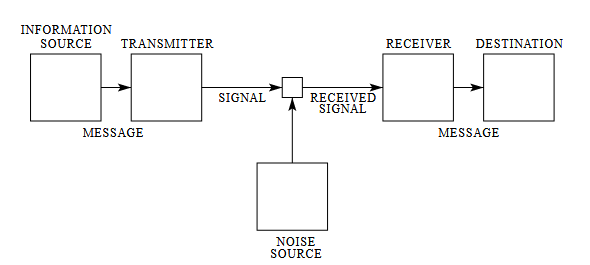
\includegraphics[width=1\linewidth]{content/pictures/shannon-weaver.PNG}
\caption{Kommunikationsmodell von Shannon / Weaver (Quelle: \cite[S. 2]{shannon_mathematical_1948})}
\label{fig:shannon-weaver-modell}
\end{figure}

Abbildung \ref{fig:shannon-weaver-modell} zeigt das wohl bekannteste Klassifikationsmodell von Shannon / Weaver. Es beschreibt jedoch keine soziale Kommunikation, sondern einen technischen Signaltransfer zwischen Sender und Empfänger. Es zeigt eine physikalische Informationsübertragung, wie z. B. ein Telefongespräch (vgl. \cite[S. 92]{scheufele_kommunikationstheorien_2004}). 

Eine Informationsquelle will eine Nachricht an ein Ziel senden. Dabei wird die Nachricht durch einen Transmitter in ein analoges/ digitales Signal umgewandelt und an ein Empfängergerät übermittelt. Innerhalb des gesendeten Signals können Störgeräusche einwirken, die ebenfalls mit übermittelt werden. Über das Empfangsgerät kann der Empfänger nun die Nachricht mitsamt Störsignal bspw. abhören.

\subsection{Kommunikationsmodell nach Osgood / Schramm}

\begin{figure}[ht]
\centering
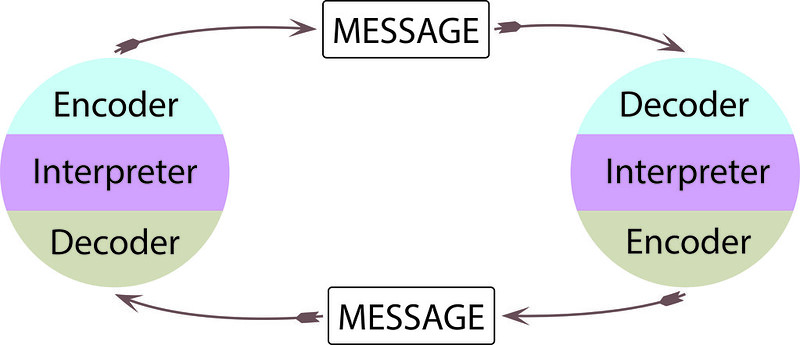
\includegraphics[width=1\linewidth]{content/pictures/osgood-schramm.jpg}
\caption{Kommunikationsmodell von Osgood / Schramm (Quelle: \cite{wrench_24_2021})}
\label{fig:osgood-schramm-modell}
\end{figure}

Das in Abbildung \ref{fig:osgood-schramm-modell} gezeigte Modell unterscheidet sich grundlegend von früheren, linearen Modellen, wie dem von Shannon / Weaver. Es zeigt stattdessen die Wechselseitige und Zirkularität von Kommunikation an. Kommunikation ist nicht nur eine einmalige Übertragung von Signalen, sondern ein kontinuierlicher Austausch, in dem beide Gesprächspartner die Bedeutung einer Botschaft gemeinsam aushandeln. Eine Antwort oder Feedback ist dabei kein optionales Element, sondern ein zentrales. Es erlaubt zudem Missverständnisse zu klären, Reaktionen einzuholen und Aussagen zu präzisieren (vgl. \cite{noauthor_osgood_2024}). 

Besonders an dem Modell ist, dass persönliche Erfahrungen der Kommunikationsteilnehmer in Form von individuellen Erfahrungen, kulturelle Prägungen, Bildung und Erwartungen in den Gesprächszyklus einfließen kann. Anhand dieser Erfahrungen erfolgt ein Codierungs / Decodierungsprozess in sprachliche und nicht-sprachliche Zeichen, welche der Empfänger interpretiert (vgl. \cite{noauthor_osgood_2024}). 

\subsection{Kommunikationsmodell nach Badura}
Als Erweiterung des Modells von Osgood und Chramm kann das Modell von Badura gesehen werden (vgl. Abbildung \ref{fig:badura-modell}).

\begin{figure}[ht]
\centering
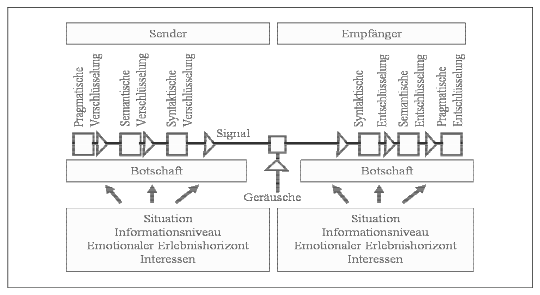
\includegraphics[width=1\linewidth]{content/pictures/badura.PNG}
\caption{Kommunikationsmodell von Badura (Quelle: \cite{badura_kommunikation_1992}, \cite[S. 93]{scheufele_kommunikation_2007})}
\label{fig:badura-modell}
\end{figure}

Das Kommunikationsmodell unterscheidet zwischen semantischen, syntaktischen und pragmatischen Aspekten der Sprache bzw. kommunikativer Botschaften. Der Rahmen in der die Kommunikation stattfindet, umfasst in diesem Modell vier Aspekte der Kommunikationssituation und zwar: dem Informationsniveau der Teilnehmer, dem emotionalem Erlebnishorizont der Teilnehmer in den jeweiligen Situationen und deren Interessen und Zielen (vgl. \cite[S. 93]{scheufele_kommunikation_2007}).

\subsection{Das Kommunikationsquadrat nach Schultz von Thun}
Während die Modelle von Shannon / Weaver oder Osgood / Schramm den Ablauf und die Zirkularität von Kommunikation erklären, geht das Kommunikationsquadrat direkt auf die inhaltliche Vielschichtigkeit jeder Botschaft ein. Sobald Menschen miteinander kommunizieren, übermitteln sie nicht nur Inhalte, sondern auch Hinweise zur Beziehung, zur Selbstdarstellung und zum kommunikativen Zweck.

\begin{figure}[ht]
\centering
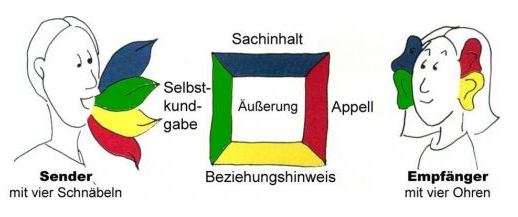
\includegraphics[width=1\linewidth]{content/pictures/Kommunikationsquadrat.PNG}
\caption{4 - Ohren Modell von Schulz von Thun (Quelle: \cite{noauthor_kommunikationsquadrat_nodate})}
\label{fig:four-ears}
\end{figure}

Das in Abbildung \ref{fig:four-ears} gezeigte Modell, auch \say{Nachrichtenquadrat} oder \say{Kommunikationsquadrat}, genannt, zeigt die vier Botschaften, die eine Nachricht gleichzeitig enthält. Diese sind die Sachinformation, bei der darüber informiert wird, um was es in der Nachricht geht. Die Selbstkundgabe, bei der der Sender Informationen über sich selbst freigibt. Dem Beziehungshinweise, in welchem Verhältnis der Sender zum Empfänger steht und den Appell, durch welchen das Ziel der Botschaft offenbart wird (vgl. \cite{noauthor_kommunikationsquadrat_nodate}).

Die gewählten Äußerungen entstammen dabei aus den \say{vier Schnäbeln} des Senders, die auf die \say{vier Ohren} des Empfängers treffen (vgl. \cite{noauthor_kommunikationsquadrat_nodate}). Schulz von Thun geht dabei davon aus, dass jede Nachricht mit vier Ohren empfangen werden (vgl \cite[S. 23]{becker_praxishandbuch_2018}). 

Dieses Modell ist im Kern ein Ausdrucksmodell der Kommunikation. Einerseits soll es dabei dabei helfen, Ursachen für mögliche Missverständnisse zu verstehen und andererseits übersieht es den Charakter der Gemeinschaftshandlung als auch den Steuerungscharakter des Sprechens (vgl \cite[S. 23]{becker_praxishandbuch_2018}). Es berücksichtigt somit nicht das Nachfragen beim Sender. Stattdessen suggeriert es, dass jede Äußerung einen einzigen wahren Bedeutungskern hätte (vgl \cite[S. 23]{becker_praxishandbuch_2018}). 

\subsection{Konversationsmaximen von Grice}
Grice erweitert die o. g. Theorien dadurch, dass nicht nur über das Gesagte die Kommunikation funktioniert, sondern auch durch das Implizierte (vgl. \cite[S. 43f]{grice1975logic}). Aus den Bedingungen unter welchen Konversationen stattfinden. In  der Regel bestehen sie nicht aus zufälligen und unzusammenhängenden Äußerungen, sondern man kann das Kooperationsprinzip ableiten. Es handelt dabei davon, dass der Gesprächsbeitrag so gestaltet werden soll, wie es der Zweck oder die Richtung des Gesprächs in dem jeweiligen Stadium verlangt (vgl. \cite[S. 45]{grice1975logic}).
Aus dieser Annahme können vier Kategorien unterschieden werden. Die Quantität (Menge der Informationen) beinhaltet, dass der (gesprochene) Beitrag so informativ wie erforderlich, jedoch nicht informativer als nötig gestaltet werden soll. Die Qualität (Wahrheit) beinhaltet die Aufrichtigkeit der Nachricht. Es darf nichts gesagt werden, was der Sprecher für falsch hält und wofür keine ausreichende Belege vorhanden sind. Unter dieser Relation wird die Relevanz der Nachricht definiert. Und zuletzt: die Modalität (Art und Weise) des Gesagten. Darunter fallen die Vermeidung von Unklar- und Mehrdeutigkeiten, sowie das Vermeiden von Ausschweifungen und die Forderung nach Ordnung (vgl. \cite[S. 45f]{grice1975logic}).

Sobald gegen eine der Maximen verstoßen wird, kann der andere Interaktionsteilnehmer davon ausgehen, dass es dafür einen Grund gibt. Hier entsteht nun die implizierte Bedeutung. Die Maximen können den Kommunikationsteilnehmern eine Interpretationshilfe geben (vgl. \cite[S. 49f]{grice1975logic}).

\subsection{Axiome der Kommunikationen nach Watzlawik et. al}
In Ergänzung zu den zuvor genannten Modellen betrachten Watzlawik, Beavin und Jackson die Grundlagen zwischenmenschlicher Kommunikation aus der systematisch konstruktivistischen Perspektive. Im Zentrum steht die Kommunikation als wechselseitiges Verhalten innerhalb sozialer Kontexte (vgl. \cite{Watzlawick2016-km}). 

Dabei wurden fünf Grundsätze (Axiome) definiert, die die menschliche Kommunikation erklären (vgl. \cite{Watzlawick2016-km}):
\begin{itemize}
    \item \say{Man kann nicht nicht kommunizieren}, dies wird über das Verhalten begründet, welches immer gegeben ist (vgl. \cite[S. 53]{Watzlawick2016-km}).
    \item \say{Jede Kommunikation hat einen Inhalts- und einen Beziehungsaspekt, derart, dass letzterer den ersteren bestimmt und daher eine Metakommunikation ist.} \cite[S. 64]{Watzlawick2016-km}
    \item \say{Die Natur einer Beziehung ist durch die Interpunktion der Kommunikationsabläufe seitens der Partner bedingt.} Die Kommunikation verläuft zirkular. (vgl. \cite[S. 69]{Watzlawick2016-km})
    \item Menschliche Kommunikation nutzt sowohl digitale als analoge Ausdrucksformen. Digitale Kommunikation ist logisch strukturiert, aber in Beziehungssituationen bedeutungsarm. Analoge Kommunikation hingegen transportiert Beziehungsinhalte wirkungsvoll, ist jedoch weniger eindeutig in der Bedeutung (vgl. \cite[S. 77]{Watzlawick2016-km}).
    \item \say{Zwischenmenschliche Kommunikationsabläufe sind entweder symmetrisch oder komplementär, je nachdem, ob die Beziehung zwischen den Partnern auf Gleichheit oder Ungleichheit beruht} \cite[S. 80]{Watzlawick2016-km}
\end{itemize}

\subsection{Gelingende Kommunikation nach Carl Rogers}
Die o. g. Modelle bezogen sich auf den strukturellen Aufbau und Regeln kommunikativen Handelns, sowie dem Aufbau der übermittelten Nachrichten. Carl Rogers ging einen Schritt weiter und beschäftigte sich damit, wie die Kommunikation der Teilnehmer gelingen kann (empathische Kommunikation). 

Er stellte dabei die drei wichtigen Prinzipien der Echtheit (Kongruenz), Empathie und Wertschätzung (Bedingungslose Akzeptanz) fest. Die Echtzeit umschreibt die Offenheit der Gesprächsteilnehmer, sowie die Vermeidung von Künstlichkeit im Verhalten dem anderen gegenüber. Dadurch soll ein Gefühl von Sicherheit entstehen. Die Empathie beschreibt das Hineinversetzten in die Lage des anderen. Dadurch soll versucht werden, die Gefühle und Gedanken aus den Perspektiven der Gesprächsteilnehmer zu verstehen. Dieses Verständnis fördert eine tiefere emotionale Verbindung. Die Wertschätzung umfasst, wie es das Wort bereits aussagt, das Wertschätzen der anderen Person, unabhängig seines Verhaltens oder Meinung. Aus der Wehrschätzung heraus sollen sich die Gesprächsteilnehmer sicher und geschützt fühlen (vgl. \cite{jesse_carl_2025}).
% Zunächst definierte er das Menschenbild über die Kernelemente der Selbstverwirklichung, Bedürfnisse, Individualitäten, Erfahrungen und Positivität (vgl. \cite{warkentin_carl_2024}). 
 
\section{Spielertypen}
Die Kommunikationswissenschaft umfasst zwar den Schwerpunkt dieser Arbeit, jedoch wurden auch ludologische Aspekte berücksichtigt. Dabei handelt es sich um die wissenschaftliche Auseinandersetzung mit dem Spielen selbst (vgl. \cite{ludologie_spielforschung_nodate}). 

Im Hinblick auf die Konzeption und Entwicklung eines Spiels ist es wichtig, die Eigenschaften des Spielsystems so zu gestalten, dass sie Begeisterung und Engagement bei der gewünschten Zielgruppe hervorrufen. Aus diesem Grund muss zunächst die Zielgruppe in verschiedene Typen eingeteilt werden. Die Ludologie unterscheidet hierfür verschiedene Spielertypen. Zwar ist nicht jeder Mensch ein \say{Spielertyp}, dennoch kann er grundsätzlich durch unterschiedliche Spielelemente angesprochen werden (vgl. \cite{ludologie_spielertypen_nodate}).

\subsection{Nach Bartle}
1996 beschäftigte sich Richard Bartle mit der Frage, welche Spielertypen in der Ludologie unterschieden werden können. Dabei ging es zunächst um Klassifizierungen von Ansätzen, die beim Spielen von sogenannten \ac{MUD}s existieren (vgl. \cite{bartle_hearts_1996}). Diese Klassifizierungen werden noch heute für die Einteilung in Spielertypen herangezogen.

Bartle unterscheidet bei der Einteilung der Spielertypen zwei grundlegende Interessen (vgl. Abbildung \ref{fig:bartle-muds}):

\begin{figure}[ht]
\centering
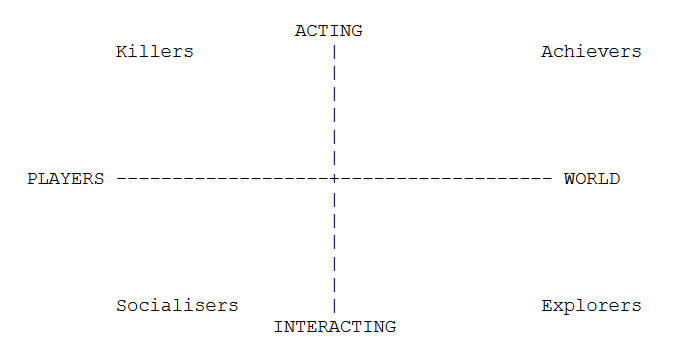
\includegraphics[width=1\linewidth]{content/pictures/basic_interests.PNG}
\caption{Interessen Graph nach Bartle (Quelle: \cite{bartle_hearts_1996})}
\label{fig:bartle-muds}
\end{figure}

Auf der X-Achse wird unterschieden, ob Spieler ihre Spielerfahrung über das Verhalten der anderen Mitspieler (Players) oder über die Spielwelt (World) definieren. Entlang der Y-Achse wird unterschieden, ob Spieler eher selbst aktiv Einfluss auf die Spielwelt nehmen möchten (Acting) oder ob sie in eine tiefere Interaktion mit ihr eingehen wollen (Interacting).

Die daraus resultierenden Typen sind:
\paragraph{Achiever}
Sie sind daran interessiert, auf die Spielwelt einzuwirken und alle ihnen gestellten Aufgaben mit Erfolg zu absolvieren. Ihr Status im Spiel ist ihnen wichtig - ebenso wie die Effizienz, mit der sie Fortschritte erzielen.

\paragraph{Explorer}
Sie wollen vom Spiel überrascht werden und intensiv mit der Spielwelt interagieren. Die virtuelle Welt löst ein Gefühl des Staunens aus, nach dem sie aktiv suchen. Sie sind stolz auf das Wissen, das sie im Spiel sammeln. Das erlangte Wissen möchten sie gerne an neue Spieler weitergeben.

\paragraph{Socialiser}
Sie wollen mit anderen Spielern interagieren, meist über Gespräche, aber auch durch ungewöhnliche oder kreative Verhaltensweisen. Andere Menschen kennenzulernen und mehr über sie zu erfahren, ist für sie wertvoller als für andere. Die Spielwelt dient dabei lediglich als Kulisse - entscheidend sind für sie die Begegnungen mit anderen Charaktere. Sie sind stolz auf Freundschaften, ihre Kontakte und ihren Einfluss.

\paragraph{Killer}
Sie sind daran interessiert, auf andere Spiele einzuwirken und mit ihnen zu interagieren - häufig ohne deren Einverständnis. Sie wollen ihre Überlegenheit gegenüber anderen Menschen demonstrieren und sind stolz auf ihren Ruf sowie ihre oft geübten Kampffähigkeiten.

(vgl. \cite{bartle_hearts_1996}).

\subsection{Erweiterte Einteilungen}
Bartle ist nicht der Einzige, der sich mit Spielertypen auseinandergesetzt hat. Seine Forschung bildet jedoch ein grundlegendes Fundament, das in der weiteren wissenschaftlichen Auseinandersetzung intensive Diskussionen innerhalb der Forschungs- und Game-Design-Community ausgelöst hat. 
\begin{quote}
    \textit{
        \enquote{Player types are not a defined concept and any categorization of players or users needs to occur within the context of a particular application or domain. Play-personas are suggested as a useful tool that can be used to put player type research into practice as part of the design process of gamified systems.}
    } 
    (\cite{dixon_player_nodate})
\end{quote}

\paragraph{Dixon} 
stellt Spieler-Personae vor, die analog zum \ac{UCD}-Prozess eingesetzt werden können. Dadurch muss im Designprozess nicht strikt zwischen Motivation, Verhalten und Vorlieben unterschieden werden, da Personae als ausführliche, erzählerische Darstellung gedacht sind (vgl. \cite{dixon_player_nodate}).

\paragraph{Bateman und Boon}
entwickelten in ihrer 2005 erschienenen Studie zur Bestimmung des ersten Modells des Demographic Game Design (DGD1) vier Spielstile, die sie durch die Einbeziehung des \ac{MBTI} ableiteten (vgl. \cite{noauthor_mbti_nodate}; \cite{bateman_21st_2005}).
% Conquerer (Eroberer), Manager, Wanderer (Wanderer) und Participant (Teilnehmer) waren dabei die vier Spielstile.
Die vier Spielstile lauteten: Conquerer (Eroberer), Manager (Manager) Wanderer (Wanderer) und Participant (Teilnehmer).

In einer zweiten Studie wurden vier hypothetische Spielstile entwickelt, die auf einer Untersuchung von \cite{berens_understanding_2000} basierten (vgl. \cite{bateman_player_2012}). Die daraus resultierenden Stile lauteten: Logistical, Tactical, Strategic und Diplomatic.

Im Kern sind diese Modelle Weiterentwicklungen bzw. Ableitungen von Bartles ursprünglicher Typologie (vgl. \cite{ludologie_spielertypen_nodate}).

\paragraph{Yee}
Nick Yee entwickelte ein empirisch fundiertes Modell zur Beschreibung von Spielmotivationen in Online-Spielen, das bis heute einen bedeutenden Einfluss auf die Ludologie hat. Anhand eines faktorenanalytischen Ansatzes untersuchte er eine Vielzahl an Daten aus Online-Umfragen und identifizierte dabei zehn spezifische Motivationsgruppen, die sich in drei übergeordnete Hauptkategorien einordnen lassen (vgl. Abbildung \ref{fig:nick_yee_motivations}):

\begin{figure}[ht]
\centering
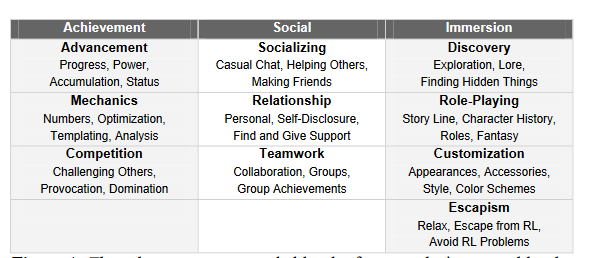
\includegraphics[width=1\linewidth]{content/pictures/nick_yee_categorizations.PNG}
\caption{Motivationsgruppen nach Nick Yee (Quelle: \cite{yee_motivations_2006})}
\label{fig:nick_yee_motivations}
\end{figure}

Die Achievement-Komponente umfasst den Fortschritt im Spiel, sowie das damit einhergehende Verlangen Macht zu erlangen, schnell voranzukommen und Symbole für Reichtum oder Status zu erwerben. Zudem besteht ein Interesse daran, die Spielmechanik zu analysieren, die Regeln und Systeme zu verstehen um die Leistung der Spielfigur zu optimieren. Auch ist der Wettbewerb spielt eine zentrale Rolle: Es besteht der Wunsch, sich mit anderen zu messen und gegen sie anzutreten.

Die soziale Komponente beschreibt das Bedürfnis nach Sozialisierung. Spieler haben Interesse daran, anderen zu helfen und sich mit ihnen zu unterhalten. Daraus entstehen Beziehungen, bei denen der Wunsch besteht, langfristige und bedeutungsvolle Bindungen zu anderen aufzubauen. Teamarbeit ist dabei gewünscht, um gemeinsame Ziele zu erreichen oder sich im Wettbewerb zu behaupten.

Die Immersion-Komponente beschreibt das Entdecken der Spielwelt und das damit verbundene Finden von Objekten sowie das Erlangen von Wissen, das den meisten anderen Spielern unbekannt ist. Rollenspiel-Elemente sind besonders wichtig, um den Spielfiguren Hintergrundgeschichten zu geben und gemeinsam improvisierte Erzählungen zu entwickeln. Der Spielavatar sollte zudem anpassbar sein, damit persönliche Vorlieben und der individueller Stil der Spieler zum Ausdruck kommen können. Die Spielwelt dient auch als Mittel um dem Alltag zu entfliehen und den Problemen der realen Welt zu entkommen.

\paragraph{weitere Modelle}
Im Zuge der fortschreitenden Forschungen entstanden weitere Modelle wie zum Beispiel das Gamer Motivation Model, das auf Basis der Forschung von Nick Yee entwickelt wurde (vgl. \cite{ludologie_spielertypen_nodate}):

\begin{figure}[ht]
\centering
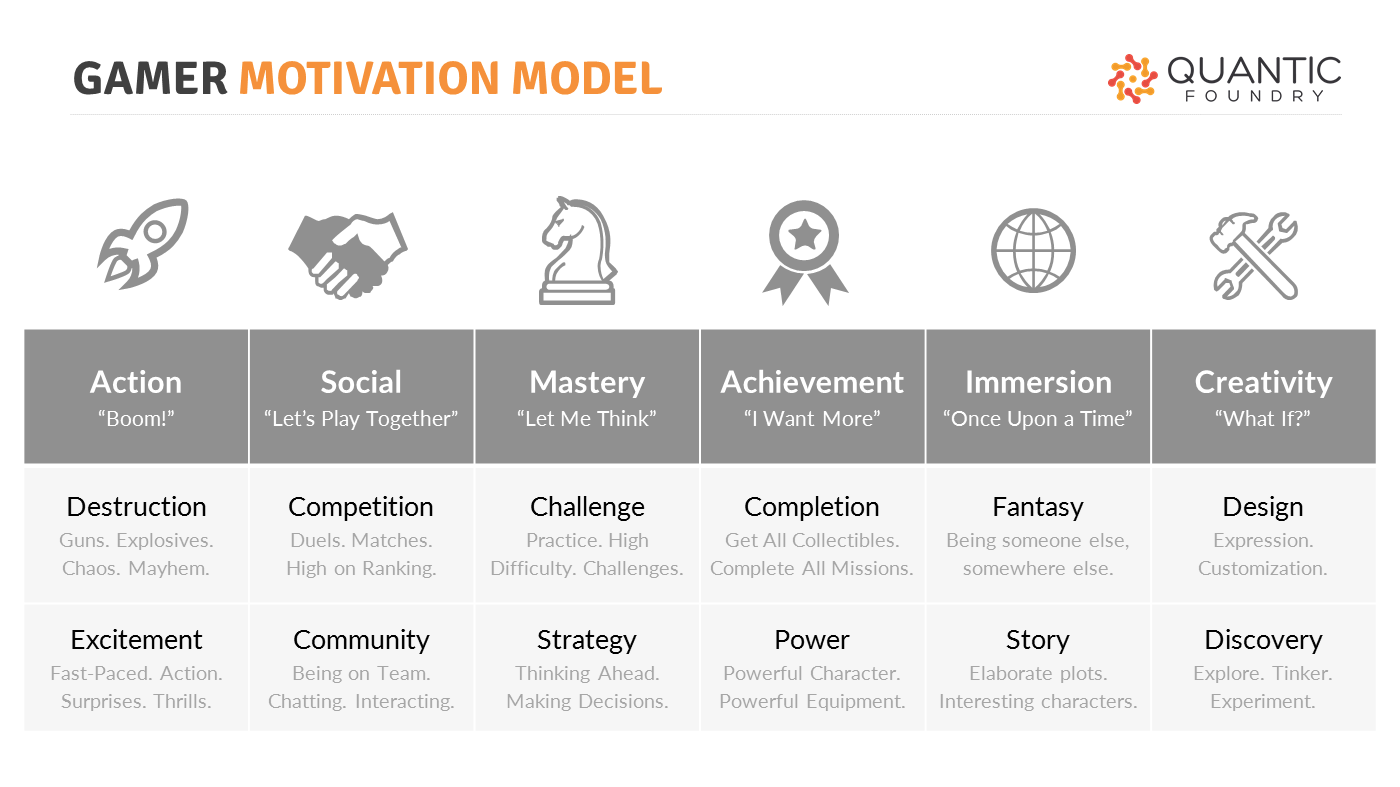
\includegraphics[width=1\linewidth]{content/pictures/gamer_motivations_model.png}
\caption{Gamer Motivation Model der QUANTIC FOUNDRY (Quelle: \cite{noauthor_quantic_nodate})}
\label{fig:gamer_motivation_model}
\end{figure}

Ein weiteres Modell, das in der Arbeit von Bateman genannt wird, ist das BRAINHEX-Model, bei dem die verschiedenen Spielertypen in hexagonaler Anordnung platziert sind (vgl. Abbildung: \ref{fig:brain-hex}):

\begin{figure}[ht]
\centering
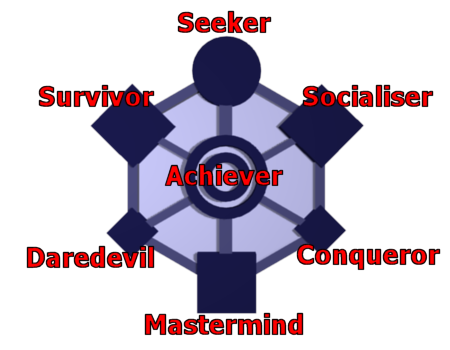
\includegraphics[width=1\linewidth]{content/pictures/brainhex-classes.png}
\caption{Brainhex-Model Darstellung von \cite{noauthor_i_nodate} nach \cite{nacke_brainhex_2013}}
\label{fig:brain-hex}
\end{figure}

\section{Multiplayer-Spiele}
Im Vergleich zu Einzelspieler-Spielen existieren bei Multiplayer-Spielen nicht nur Unterschiede im Genre, sondern auch in den Spielrollen (Symmetrie / Asymmetrie) sowie in den Spielzeitpunkten, zu denen die Spielteilnehmer an ihrem Spielfortschritt weiterarbeiten (Synchron / Asynchron). [Hier wäre eine Quelle noch gut]. Auf dem Spielemarkt existieren außerdem Multiplayer-Spiele, die unterschiedliche Medientechniken verwenden. Teilweise dienen diese Medientechniken dazu, Cross-Plattform Funktionalität zu gewährleisten (vgl. \cite{noauthor_baldurs_nodate}), oder sie sind integrale Bestandteil des Gamedesigns (vgl. \cite{noauthor_keep_nodate}).

Da im Kontext von \say{Connecting-Minds} die Spieler zeitgleich in einer Sitzung gemeinsam spielen, wird im Folgenden auf die Symmetrie und Asymmetrie von Computer- und Videospielen eingegangen.

\subsection{Symmetrische Multiplayer}
Symmetrische Spiele sind solche, bei denen alle Spieler die gleichen Spielregeln haben und das gleiche Spielziel verfolgen. Viele traditionelle Spiele wie Schach sowie Computer- und Videospiele wie \say{Mario Kart} oder \say{Minecraft} sind symmetrische Multiplayer-Spiele, bei denen für jeden Spieler das gleiche Ziel gilt (vgl. \cite[S. 12]{adams_fundamentals_2013}); (vgl. \cite{nintendo_mario_1992}); (vgl. \cite{noauthor_willkommen_2009}). 


\subsection{Asymmetrische Multiplayer}
Asymmetrische Spiele hingegen können unterschiedlichen Spielern unterschiedliche Regeln zugestehen und ggf. verfolgen die Spieler unterschiedliche Ziele (vgl. \cite[S. 12]{adams_fundamentals_2013}). Sie sind sowohl in kooperativen als auch kompetitiven Spielen weit verbreitet und werden bspw. in Form verschiedener \say{Helden} oder \say{Klassen} umgesetzt. So gibt es z.B. in \say{Overwatch} oder \say{League of Legends}  unterschiedliche \say{Support}-Charaktere, deren Aufgabe es ist das Team zu heilen (vgl. \cite{smilovitch_birdquestvr_2019}); (vgl. \cite{noauthor_league_2025}); (vgl. \cite{noauthor_overwatch_nodate}). 
Außerdem ermöglichen asymmetrische Spiele, dass Spieler mit unterschiedlichen Fähigkeiten und Fähigkeitsniveaus gemeinsam spielen können. Ein asymmetrisches Design kann zudem die Inklusivität in Spielen fördern (vgl. \cite{smilovitch_birdquestvr_2019}).

\subsection{Hybride Multiplayer}
Wie Lotz in ihrer Bachelor-Arbeit beschrieben hat, unterscheiden sich Multiplayer auch in der verwendeten Medientechnik (vgl. \cite[S. 6f]{lotz_konzeption_2021}). Sogenannte hybride Spiele wie \say{New Super Mario Bros U} (vgl. \cite{noauthor_mario_nodate-1})

\begin{figure}[ht]
\centering
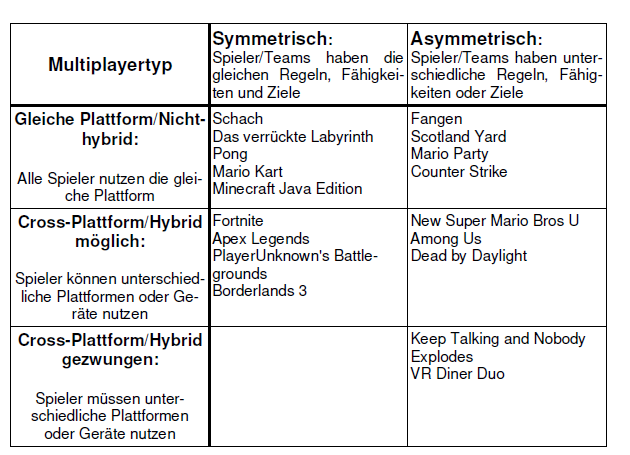
\includegraphics[width=1\linewidth]{content/pictures/lotz_hybrid_multiplayer.PNG}
\caption{Unterscheidung Multiplayertypen (Quelle: \cite[S.6]{lotz_konzeption_2021})}
\label{fig:lotz_multiplayer_types}
\end{figure}

Wie Abbildung \ref{fig:lotz_multiplayer_types} zeigt, können Multiplayer-Spiele hinsichtlich ihrer Medientechnik in drei Kategorien eingeteilt werden.
Spiele wie \say{Mario Kart} oder \say{Minecraft} können nur auf der gleiche Plattform gespielt werden. Bei Spielen wie \say{Among Us} oder \say{Fortnite} ist die Plattform, auf der gespielt wird, nicht relevant, da eine Cross-Play-Funktionalität gegeben ist. Jeder kann mit Spielern auf der Plattform spielen, die er zu zuhause hat. Die dritte Kategorie umfasst Spiele, bei denen die Spieler gezwungen werden, unterschiedliche Plattformen zu nutzen. In \say{Keep talking and nobody explodes} ist dies der Kern des Gamedesigns.

\section{Spielweisen von Multiplayer-Spielen}
Nachdem die unterschiedlichen Strukturen und technischen Formen von Multiplayer-Spielen behandelt wurden, ist es nun wichtig, die verschiedenen Spielweisen zu betrachten. Multiplayer-Spiele können dabei in drei Hauptspielformen unterteilen:
In kompetitive, kollaborative und kooperative Spielweisen (vgl. \cite[S. 25f]{zagal_collaborative_2006}).

\subsection{Kompetitiv}
Kompetitive Spiele sind solche, bei denen Spieler oder Teams gegeneinander antreten, um ein bestimmtes Ziel zu erreichen, wobei der Erfolg des einen oft den Misserfolg des anderen bedeutet. In diesen Spielen ist das Spiel selbst neutral und agiert nicht aktiv im Wettbewerb (vgl. \cite{noauthor_game_2014}), (vgl. \cite[S. 25]{zagal_collaborative_2006}).

\subsection{Kollaborativ}
Kollaborative Spiele sind solche, bei denen alle Spieler - ähnlich wie in Kooperationsspielen - gemeinsam gegen das Spiel verlieren können. Allerdings können sie nicht gemeinsam gewinnen. Diese Spiele sind im Kern meist kompetitiv, beinhalten jedoch die Möglichkeit einer kollektiven Niederlage. Die Spieler müssen zu einem gewissen Maß zusammenarbeiten, um nicht zu verlieren (vgl. \cite{noauthor_game_2014}), (vgl. \cite[S. 25]{zagal_collaborative_2006}).

\subsection{Kooperativ}
Bei Kooperationsspielen ist es möglich, dass alle Spieler gemeinsam gegen das Spiel verlieren oder gemeinsam gewinnen können. Ein Sieg wird erreicht, wenn das Spiel gemeinsam \say{besiegt} wird oder dadurch dass ein festgelegtes Ziel kollektiv oder individuell erreicht werden kann (vgl. \cite{noauthor_game_2014}), (vgl. \cite[S. 25]{zagal_collaborative_2006}).

\section{Augmented Reality}

\ac{AR} stellt eine Form virtueller Umgebungen (\ac{VE}) dar, bei der im Gegensatz zur vollständigen Immersion in rein virtuelle Welten, wie es in \ac{VR} der Fall ist, die Umgebung weiterhin sichtbar bleibt. Virtuelle Objekte werden dabei über die physische Welt gelegt und mit ihr kombiniert, sodass eine erweiterte Wahrnehmung entsteht. Es gewährleistet außerdem eine Interaktion mit den räumlich (\ac{3D}) registrierten virtuellen Inhalten in Echtzeit. Die technische Umsetzung kann dabei über monitorbasierte Schnittstellen, monokulare Systeme oder durchsichtige \ac{HMD}s erfolgen (vgl. \cite[S. 2f]{azuma_survey_1997}).



% \cite{el_barhoumi_assessment_2022} 

% Es gibt drei verschiedene Ansätze, wie virtuelle Objekte in die virtuelle Szene der Anwendung platziert werden können:
% \begin{itemize}
%     \item Marker basiertes \ac{AR}
%     \item Markerloses \ac{AR}
%     \item Hybride \ac{AR} Ansätze
% \end{itemize}
% Der Marker-Basierte Ansatz verwendet einen bestimmten Marker um das \ac{3D}-Objekt an eine bestimmte Position zu binden. Dies kann entweder über eine Hyperlink Verknüpfung oder Visuell-Basierenden Markern geschehen. Bei der Hyperlink-Verknüpfung wird bein physisches Objekt mit einem Web-basierendem Inhalt durch graphische Tags oder Radiofrequenz-Identifikationssysteme verbunden. Die visuell-basierte Methode funktioniert durch das erkennen und verarbeiten von bestimmten Markern, wie physische Objekte in der Umgebung oder Papier-basierende Muster, durch die Kamera (vgl. \cite[S. 3f]{el_barhoumi_assessment_2022}).

% Der Markerlose Ansatz lässt sich in zwei verschiedene Typen unterteilen. Das sensorbasierte Tracking nutzt entweder das magentische Tracking-Verfahren, bei dem ein elektromagnetisches Feld und Sensoren verwendet werden um die Position und Orientierung in Echtzeit zu bestimmen. Es funktioniert unabhängig von Sichtverbindungen und ist unempfindlich gegenüber optischen Störungen. Es hat allerdings eine begrenzte Reichweite und ist störanfällig gegenüber Magnetfeldern. Das interiale Tracking verwendet.

% Die Kernaspekte der \ac{AR} beziehen sich darauf, dass die physische Welt durch digitale Informationen ergänzt werden kann, indem eine digitale Sicht über sie gelegt wird. Diese Informationen können 

Im Vergleich zur \ac{VR}, das eine voll-immersive Umgebung erstellt, erweitert die \ac{AR} die eigene Realität und bietet dadurch die Möglichkeit, dass sich die Nutzer frei in der Welt bewegen können und auch immer noch mit der echten Welt interagieren können (vgl. \citealp[S. 79]{billinghurst_survey_2015}; \citealp[S. 1]{stefanidi_meaningful_2024}).

\subsection{Abgrenzung der Begriffe}
% \ac{AR} und \ac{VR} werden 
In der Vergangenheit und aktuell wird in der wissenschaftlichen Forschung nach Konzepten und Möglichkeiten der Integration und Verbesserung von \ac{AR} und \ac{VR} gesucht. Damit zwischen diesen Begriffen und den weiteren in der Forschung angewandten Begriffen \ac{MR} oder \ac{XR} unterschieden werden kann, wurde von  \cite{milgram_taxonomy_1994} das Konzept des \say{\ac{VC}s} entworfen (vgl. Abbildung \ref{fig:virtuality-continuum}).

\begin{figure}[ht]
\centering
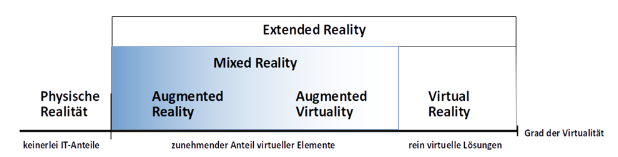
\includegraphics[width=1\linewidth]{content/pictures/virtuality-continuum_upscaled.PNG}
\caption{Vereinfachte Darstellung eines "Virtuality Continuums" (Quelle: \citealp[S. 9]{knoll_augmented_2022}; Modifiziert nach \citealp[S. 3]{milgram_taxonomy_1994})}
\label{fig:virtuality-continuum}
\end{figure}

Auf der linken Seite des \ac{VC}s befindet sich das reale Umfeld (\ac{PR}). Auf der entgegenfliegenden rechten Seite liegt die virtuelle Umgebung (\ac{VR}). Je weiter von der Seite der \ac{VR} nach links in die Richtung der \ac{PR} entgegen der Richtung der Virtualität gegangenen wird, desto häufiger werden virtuelle Elemente über die reale Welt gelegt. Die \ac{PR} besteht dabei ausschließlich aus realen Objekten. Durch die \ac{AR} können nun virtuelle Objekte über die reale Welt überlagert und erweitert werden. Bei der \ac{AV} befindet sich der Benutzer in einer virtuellen Umgebung, bei der etwas aus der realen Welt hinzugefügt wird. In der \ac{VR} befindet sich der Nutzer in einer vollständig künstlich geschaffenen Umgehung, in der er mit der Umgebung interagieren kann (vgl. \citealp[S. 3]{milgram_taxonomy_1994}; \citealp[S. 8f]{knoll_augmented_2022}; \citealp[S. 3]{zuniga_gonzalez_making_2021}). 

Die \ac{XR} umfasst alle Ausprägungen, bei denen virtuelle Elemente eingesetzt werden. Die \ac{MR} umfasst die Bereiche, in denen die virtuelle Welt die physische Welt überlagern, oder die physische Welt in der virtuellen Welt sichtbar ist. 
% Die \ac{MR} umfasst nun die Gebiete der \ac{AR} und \ac{AV}. 

\subsection{Technologische Umsetzungen}
% Die virtuelle Welt kann über verschiedene Technologien 
Die Einbettung der virtuellen Elemente in die physische Umgebung kann über verschiedene Techniken erfolgen. Die bekanntesten davon sind mitunter mobile Displays (Smartphone-Bildschirme oder Tablets), \ac{HMD}s oder Projektionssysteme. Im folgenden werden diese unterschiedlichen Technologien vorgestellt.
\begin{figure}[ht]
\centering
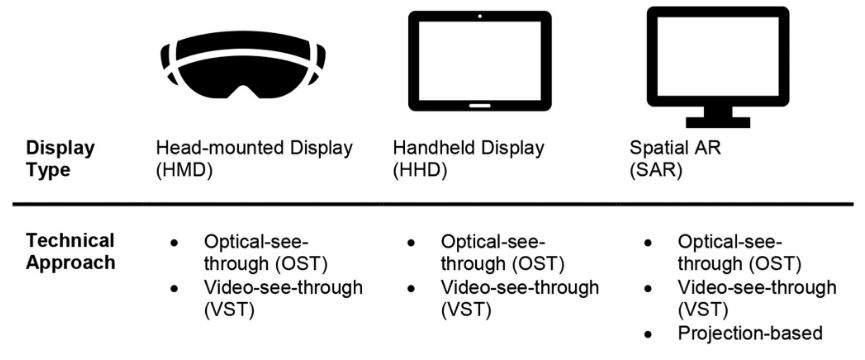
\includegraphics[width=1\linewidth]{content/pictures/devices.PNG}
\caption{Klassifizierungen von Augmented Reality Displays (Quelle: \citealp[S. 315]{leins_comparing_2024})}
\label{fig:ar-classes}
\end{figure}
\paragraph{Handheld Augmented Reality}
% In einer Hand haltbare Geräte eignen  sich gut für \ac{AR}-Anwendungen. Die Derzeitige Hardware haben 
\begin{figure}[ht]
\centering
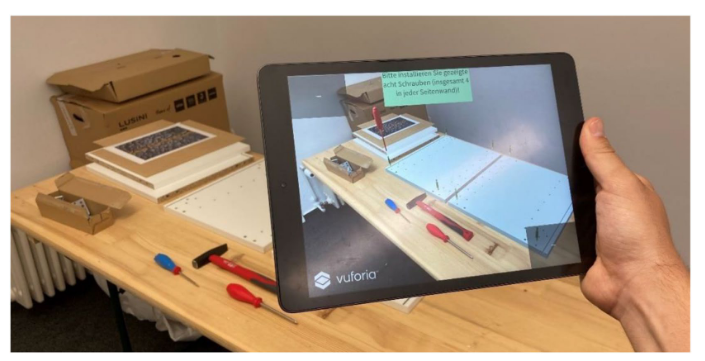
\includegraphics[width=0.5\linewidth]{content/pictures/handheld-ar.PNG}
\caption{Handheld-AR Display (Quelle: \citealp[S. 318]{leins_comparing_2024})}
\label{fig:handheld-ar}
\end{figure}

\ac{HAR} erfolgt über Handheld-Displays, die der Benutzer in der Hand halten kann (vgl. Abbildung \ref{fig:handheld-ar}). Sie verwenden Video see-through Techniken, um virtuelle Objekte über die reale Umgebung zu legen. Um dies zu ermöglichen, nutzen sie Sensoren, wie digitale Kompasse und GPS-Geräte ein um ihre Ausrichtung und Pose zu bestimmen (vgl. \citealp[S. 347]{carmigniani_augmented_2011}).

\paragraph{Head-Mounted-Devices}

\begin{figure}[ht]
\centering
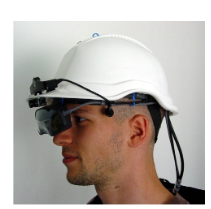
\includegraphics[width=0.5\linewidth]{content/pictures/hmd-ar.PNG}
\caption{Head-Mounted-Display (Quelle: \citealp[S. 4]{reitmayr_location_2003})}
\label{fig:hmd-ar}
\end{figure}

Bei einem \ac{HMD} trägt der Anwender ein Displaygerät auf dem Kopf oder als Teil eines Helmes (vgl. Abbildung \ref{fig:hmd-ar}), das ihm sowohl Bilder der realen als auch virtuellen Umgebung über das Sichtfeld legt. Sie können entweder video-see-through oder optisches see-through oder über monokulare- bzw. binokulare Displayoptiken verfügen (vgl. \citealp[S. 346]{carmigniani_augmented_2011}).

Video see-through Systeme setzen voraus, dass der Nutzer zwei Kameras auf dem Kopf trägt, und die Bilder aus beiden Perspektiven verarbeitet werden. Dabei werden die Bilder der Kameras (der \say{reale Teil}) zusammen mit der virtuellen Szene und der enthaltenen virtuellen Objekte verrechnet. Dieser Ansatz benötigt viel Rechenleistung (bsp.: \cite{noauthor_vive_nodate}). Optische see-through Systeme hingegen benötigen nicht so viel Rechenleistung, da eine Halbspiegeltechnologie verwendet wird, um die Sicht auf die reale Umgebung zu ermöglichen und virtuelle Elemente grafisch zu überlagern (vgl. \citealp[S. 346f]{carmigniani_augmented_2011}).

\paragraph{Spatial Augmented Reality}
\begin{figure}[ht]
\centering
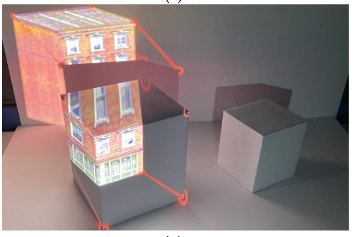
\includegraphics[width=0.5\linewidth]{content/pictures/spatial-ar.PNG}
\caption{Spatial Augmented Reality (Quelle: \citealp[S. 7]{jin_bim-based_2020})}
\label{fig:spatial-ar}
\end{figure}

\ac{SAR} nutzt Videoprojektoren und weitere Tracking-Technologien um grafische Informationen direkt auf physische Objekte zu projizieren, ohne dass der Benutzer ein Display tragen oder führen muss (vgl. Abbildung \ref{fig:spatial-ar}). Außerdem trennen sie den Großteil der Technologie vom Benutzer und integrieren sie in die Umgebung (vgl. \citealp[S. 348]{carmigniani_augmented_2011}).

Es gibt drei verschiedene \ac{SAR}-Ansätze. Beim Bildschirmbasiertem Video see-through wird kostengünstige handelsübliche Hardware benutzt. Allerdings ist dieser Ansatz nur für stationäre Anwendungen geeignet. Räumliche optische see-through Bildschirme nutzen optische Komponenten wie Spiegelstrahler oder transparente Bildschirme, um Bilder direkt im Raum auszurichten. Sie sind jedoch ebenfalls nicht mobil einsetzbar. Projektorbasierte Displays projizieren Bilder direkt auf reale Oberflächen und ermöglichen so eine nahtlose Integration virtueller Inhalte in die physische Umgebung (vgl. \citealp[S. 348]{carmigniani_augmented_2011}).

\subsection{Platzierungsmethoden virtueller Objekte}



\section{Netzwerkinfrastrukturen}\label{sec:basics-network-structures}
Um ein Multiplayer-Spiel entwickeln zu können, muss zunächst geklärt werden, wie die Netzwerkinfrastruktur der Anwendung aufgebaut sein soll. Es existieren zahlreiche Ansätze, die jeweils für verschiedene Anwendungszwecke konzipiert sind.

\subsection{Distributed Authority}
Bei einer \say{Distributed Authority}-Netzwerktopologie übernimmt jeder im Netzwerk verbundene Spielclient gemeinsam jeweils die Verantwortung für das Erstellen und Verwalten von Objekten im Netzwerk. Jeder Client simuliert dabei seinen Teil der Spielwelt selbst und steuert Objekte über die er Autorität besitzt.
Damit Positionen und andere relevanten Daten an alle anderen Clients im Netzwerk weitergeleitet werden können, wird ein zentraler, leichtgewichtiger Statusdienst verwendet, der ausschließlich für die Verteilung der notwendigen Informationen zuständig ist, ohne selbst die Anwendung zu simulieren (vgl. \cite{noauthor_distributed_2025}).

\begin{figure}[ht]
\centering
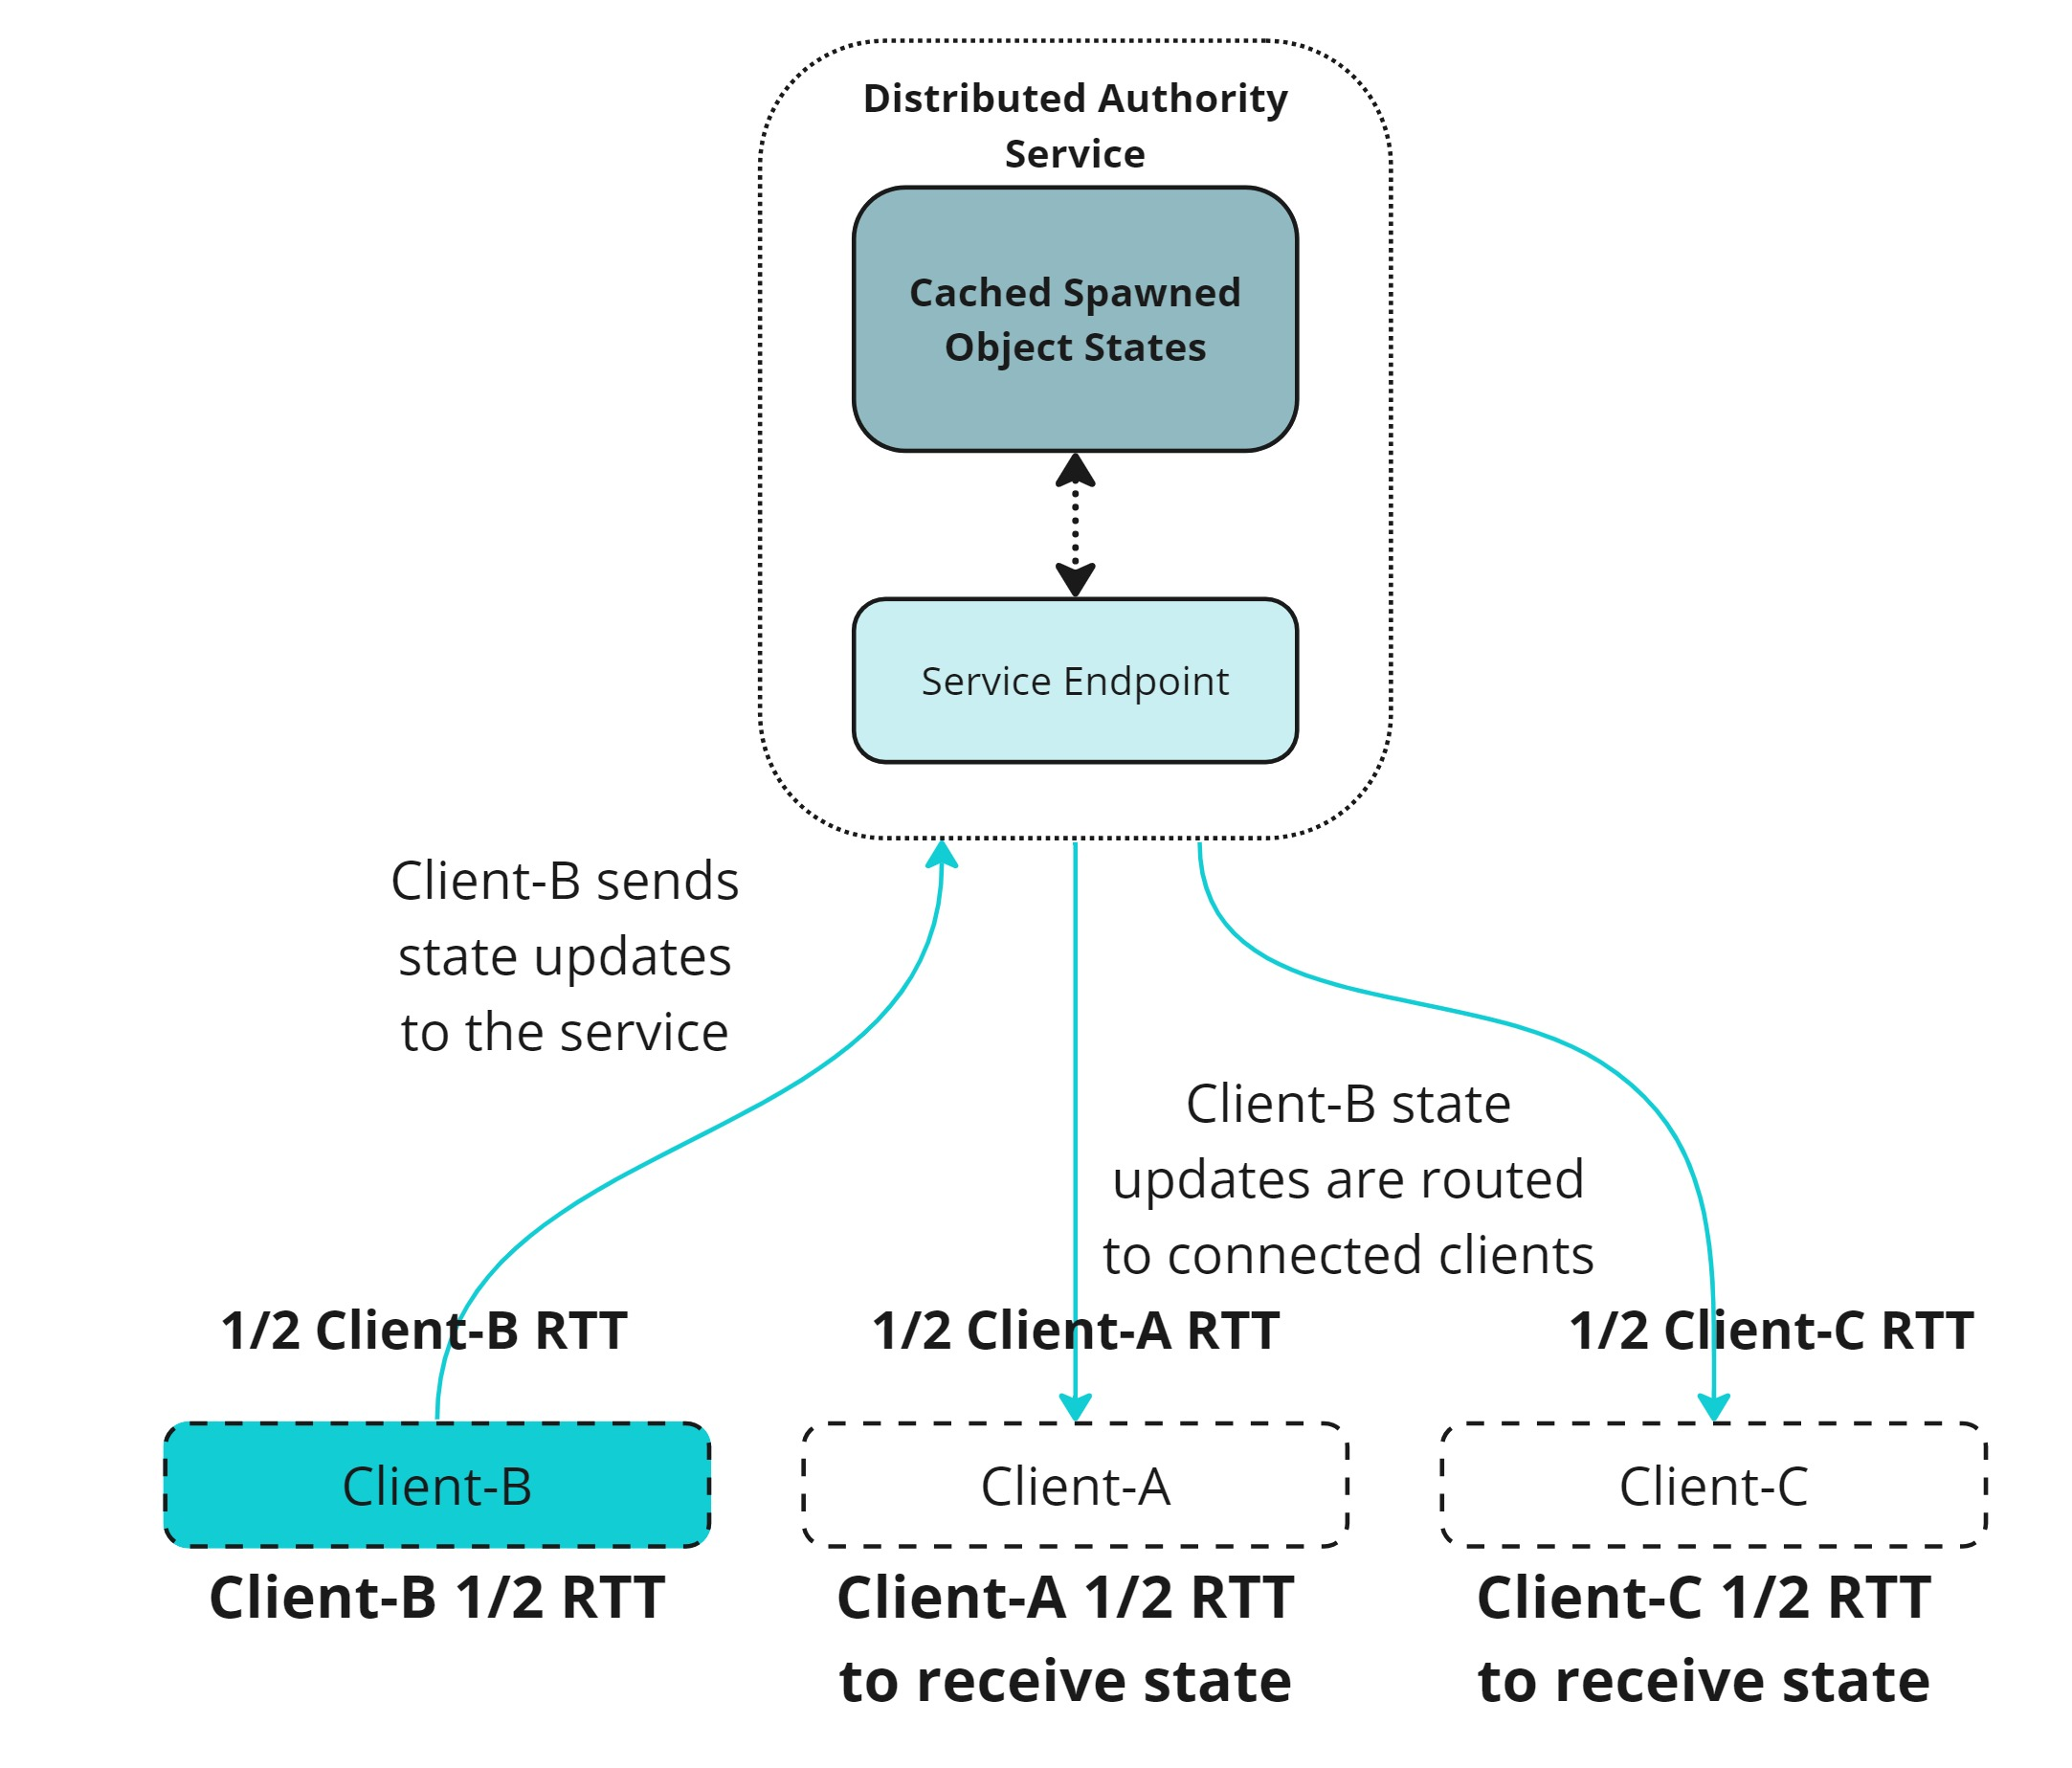
\includegraphics[width=1\linewidth]{content/pictures/distributed-authority-service.jpg}
\caption{Netzwerktopologie der Distributed Authority (Quelle: \cite{noauthor_distributed_2025})}
\label{fig:distributed_authority_topology}
\end{figure}

Spiele wie \say{Journey}, \say{God of War: Ascension}, \say{Mercenaries 2}, \say{GTA: Online}, \say{Dark Souls} und \say{Destiny} nutzen diese Netzwerkinfrastruktur. Häufig kommt diese Topologie zum Einsatz, wenn ein bestehendes Single-Player um eine Multiplayer-Komponente erweitert werden soll (Journey, GTA und Dark Souls), ohne den Kern des Quellcodes grundlegend umzustrukturieren. Diese Architektur erfordert keinen dedizierten Server, eignet sich für Spiele mit großen, offenen Spielwelten (Dark Souls, GTA) und kommt häufig zum Einsatz, wenn keine deterministische Physik benötigt wird bzw. kein vollständig deterministisches Spielkonzept vorliegt. Sie eignet sich zudem besonders für Spiele, bei denen die Prozessorleistung (z.B. durch Physiksimulationen) stark beansprucht wird. Für Spiele mit kooperativen Spielmechaniken, leichten kompetitiven Elementen oder innovativen Multiplayer-Ideen ist diese Infrastruktur eine sinnvolle Wahl (vgl. \cite{noauthor_choosing_2024}).

\subsection{Pure Client/Server}
Bei der Client-Server-Architektur übernimmt ein zentraler Server die Hauptsimulation und verwaltet alle wesentlichen Aspekte des Spiels. Dazu gehören unter anderem die Physiksimulation, das Erzeugen und Entfernen von Objekten sowie die Autorisierung von Anfragen der Clients. Aus Sicht der Clients besitzen diese lediglich die Anwendung, über die sie sich mit dem Server verbinden. Sie erhalten über diese Verbindung die Darstellung des Spiels (vgl. \cite{noauthor_client-server_2024}):
\paragraph{Ein dedizierter Server} bildet eine eigenständige Instanz, die ausschließlich dem Spielbetrieb dient (vgl. Abbildung \ref{fig:dedicated_server}).

\begin{figure}[ht]
\centering
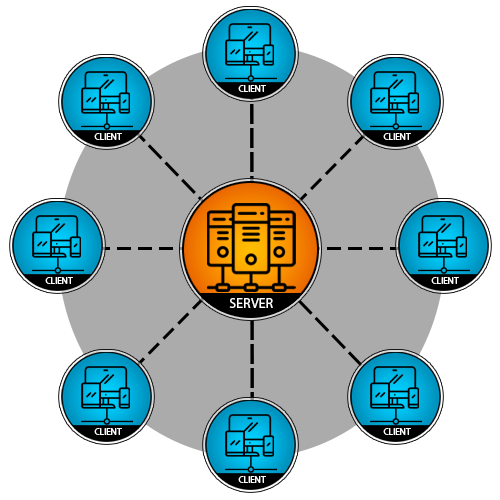
\includegraphics[width=1\linewidth]{content/pictures/ded_server-d5369721966357b9b4d5e1fa96b05b22.png}
\caption{Client-Server-Architektur mit dediziertem Server (Quelle: \cite{noauthor_network_2024})}
\label{fig:dedicated_server}
\end{figure}

\paragraph{Ein Client gehosteter Server} läuft auf demselben Gerät wie die dazugehörige Client-Anwendung (vgl. Abbildung \ref{fig:client_server}).

\begin{figure}[ht]
\centering
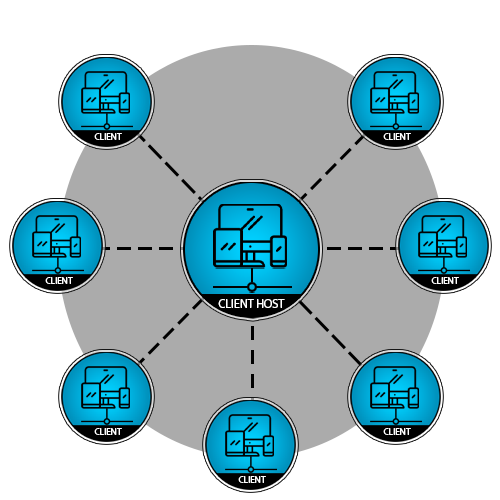
\includegraphics[width=1\linewidth]{content/pictures/client-hosted-16be0b1c9b5020f21325b1e6a7beca73.png}
\caption{Client hosted Server (Quelle: \cite{noauthor_network_2024})}
\label{fig:client_server}
\end{figure}

% \subsection{Client-Side Prediction and Lag Compensation}

% Spiele wie \say{Counterstrike}, \say{Call of Duty}, \say{Valorant} und \say{Apex legends} verwenden ein auf dem klassischen Quake-Modell basierendem Netzwerkmodell. Der Spieler steuert dabei lokal im eigenen Client, auf dem die volle Simulation läuft, ohne dabei Verzögerungen beim Laufen oder Schießen zu haben. Der Server nimmt die Eingaben samt Zeitstempel des Clients entgegen und verteilt diesen \say{State} zurück. Bspw. das Inventar, Munition oder Feuerraten. Die Korrekturen des \say{State}s werden rückwirkend auf den Client angewandt, der den Zustand bis zur aktuellen Zeit wieder herstellt (\say{Client-Side Prediction}). Schüsse und der damit einhergehende Schaden wird auf dem Server ausgewertet und an die Clients übergeben. Um das Spielerlebnis reaktionsschnell und präzise zu gestatlten, nutzt der Server ein \say{Lag Compensation} Verfahren, bei dem er anhand gespeicherter Zustände die Welt aus der Sicht der Clients zum Schlusspunkt rekonstruiert wird (vgl. \say{}.

\subsection{Peer-to-Peer}
Das \ac{P2P}-Architektur-Modell verbindet jeden Spieler direkt mit allen anderen. Über diese Verbindungen werden Daten zu Spielzuständen und Ereignissen ausgetauscht. Im \say{reinen} \ac{P2P}-System gibt es keinen zentralen \say{Host}. Stattdessen ist jeder Client dafür verantwortlich, seinen eigenen Avatar (oder seine Einheiten) zu verwalten und erhält gleichzeitig Updates von den anderen Clients (vgl. \cite{mygames_unity_2024}). Abbildung \ref{fig:p-2-p} zeigt die entsprechende Topologie.

\begin{figure}[ht]
\centering
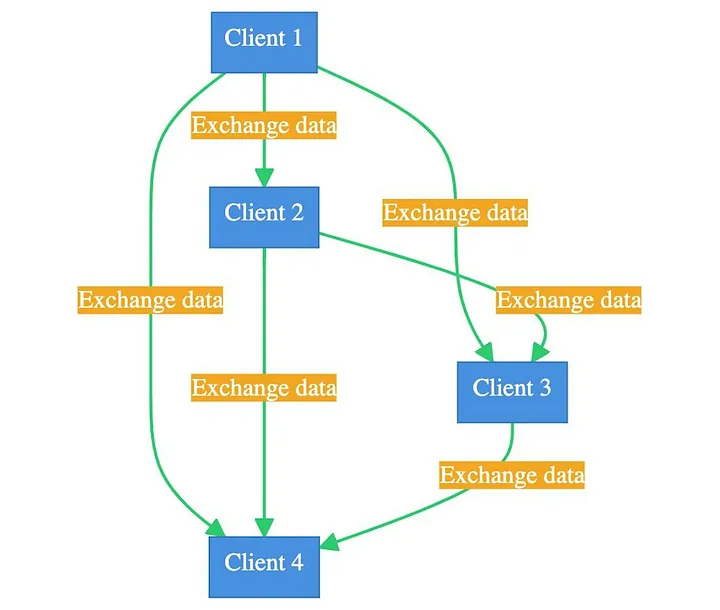
\includegraphics[width=1\linewidth]{content/pictures/0_poGQC2fWQ3tPWPwT.png}
\caption{Peer-to-Peer Infrastruktur (Quelle: \cite{mygames_unity_2024})}
\label{fig:p-2-p}
\end{figure}


\subsection{Relay-Server}
Der Relay-Dienst ermöglicht Multiplayer-Unterstützung ohne die Notwenigkeit eines dedizierten Spielserver. Dabei wird die Kommunikation zwischen den Spielern über sogenannte Relay-Server weitergeleitet. Nachrichten werden mithilfe einer latenzarmen Datagramm-Übertragung übermittelt, sodass keine direkte Verbindung zwischen den einzelnen Spielern erforderlich ist (vgl. \cite{noauthor_relay_nodate}).

\begin{figure}[ht]
\centering
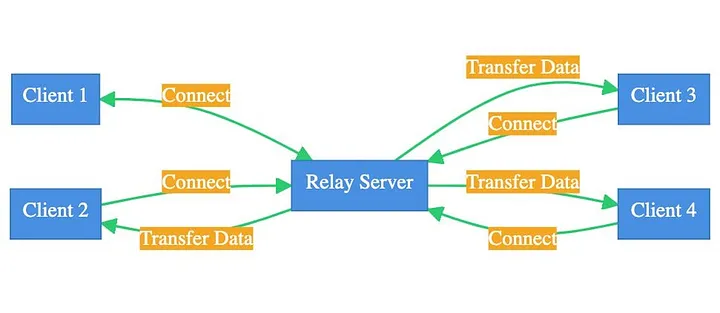
\includegraphics[width=1\linewidth]{content/pictures/0_o7LJU1ImxPHIM5Ej.png}
\caption{Relay-Server Infrastruktur (Quelle: \cite{mygames_unity_2024})}
\label{fig:relay-server}
\end{figure}

% \subsection{Verwendete Kommunikationsprotokolle}
% [überlegung hier noch die protokolle erwähnen]


\chapter{Erforschung von Anwendungen zur Kommunikationsforschung}

% \section{Verwandte Arbeiten}\label{sec:related-works}
In der \ac{CSCW} und \ac{HCI} bzw. \ac{CHI} existieren bereits diverse Arbeiten zu Multiplayer-Spielen, Effekt von Computerspiele auf das soziale Beisammensein der Spieler und welche Aspekte aus dem Gamedesign dafür verantwortlich sind.

Im Zentrum steht dabei häufig die Frage, wie Spiele soziale Interaktionen fördern oder hemmen, sowohl im kompeteiven als auch im kollaborativen Kontexten.

Video- und Computerspiele im Allgemeinen können einen positiven Einfluss auf das Miteinander haben. So untersuchte \cite{mason_friends_2013} wie wichtig Freundschaften für den Erfolg von Einzelpersonen und Teams in komplexen kollaborativen Umgebungen sind. Sie fanden heraus, dass Freundschaften einen großen Einfluss auf die verbesserte individuelle- und Teamleistung haben. Spieler richten sich dabei nach sozialen Gelegenheiten aus, sodass verborgene Freundschaftsbeziehungen direkt abgeleitet werden konnten. Kern der Studie war dabei der Online Multiplayer First-Person-Shooter \say{Halo: Reach} bei dem Spieler des Spiels eine anonyme Online Umfrage Fragen ausfüllen mussten. 

Doch soziale Dynamiken verlaufen nicht immer so positiv wie erhofft. Andere Untersuchungen zeigen ein differenzierteres Bild des Zusammenspiels in Onlinewelten.

So argumentiert \cite{ducheneaut_alone_2006} anhand einer Langzeitstudie zu \say{World of Warcraft}, dass soziale Aktivitäten in \ac{MMOG}s, oft überschätzt werden. Die meisten Spieler sind zwar von anderen umgeben, interagieren jedoch nur selten aktiv miteinander. Sie spielen häufig \say{allein zusammen}. Vor allem in den Quests zum Anfang ist das oft der Fall. Erst durch langfristige soziale Strukturen wie Gilden entstehen nachhaltige Bindungen und echte Zusammenarbeit.

Damit jedoch solche sozialen Beziehungen überhaupt entstehen können, ist es essenziell, dass Spiele die Aufmerksamkeit und das Interesse der Spielenden wecken - ein Aspekt, der unter dem Begriff \say{Player Engagement} intensiv erforscht wird.

\cite{rashed_review_2025} fassen in ihrer Überblickasarbeit unterschiedliche Methoden zur Schätzung des Spieler-Engagements zusammen. Ihr Ziel war es, über verschiedene Messmethoden wie EEG, Mimik, Eye Tracking und Spieler-Verhalten hinreichend eindeutige Daten zu sammeln um darüber eine Aussage über das Engagement treffen zu können. Die Validierung der Ergebnisse, da das Engagement subjektiv ist, ist schwer um objektiv eine \say{Ground Truth} Aussage treffen zu können.  \cite{yu_video_2023} verfolgten einen anderen Ansatz. Sie versuchten nicht nur auf das Engagement der Spieler einzugehen, sondern erforschten direkt im Bereich Zusammenarbeit und Kollaborative Fähigkeiten. Sie untersuchten kommerzielle Multiplayer-Spiele um Konzepte und Spielmechaniken zu identifizieren, die von Game-Designern zur Förderung von kooperativen Spielen genutzt werden können. Im Zuge der Forschung entwickelten sie kleine Prototypen und führten mit ihnen kleine Studien durch. 

Einige Studien gehen noch einen Schritt weiter und untersuchten nicht nur Engagement, sondern die spezifischen Bedingungen erfolgreicher Kooperation in Spielen - insbesondere durch das Design asymmetrischer Rollenverteilungen.

So zeigen die Arbeiten von \cite{harris_beam_2014}, \cite{harris_leveraging_2016} und \cite{harris_asymmetry_2019}, dass asymmetrische Spielkonzepte - bei denen sich Rollen, Fähigkeiten und Ziele der Spielenden unterschieden - einen positiven Einfluss auf die Zusammenarbeit hat. Untersucht werden dabei die Faktoren \say{Interdependence}, \say{Degrees of Interdepencene} sowie Mechaniken der Asymmetrie und Abhängigkeiten der Anwendungen. Ein asymmetrisches Spielkonzept ermöglicht außerdem eine Integration bzw. Inklusion von Spielergruppen mit eingeschränkten Fähigkeiten (vgl. \cite{goncalves_exploring_2021}). Für die Entwicklung von Spielen, die für die gesamte Familie gedacht sind, eignet es sich ebenfalls (vgl. \cite{pais_promoting_2024}).

Die Arbeiten von Harris et. al. dienen als Grundlage für die weitere Entwicklung des Game Designs für asymmetrische Multiplayer-Spiele. So identifizierte \cite{guimaraes_rocha_game_2008} verschiedene kooperative Design-Pattern, die in der weiteren Forschung und deren Spielumsetzung anklang fanden. In der Arbeit von \cite{emmerich_impact_2017} werden drei der definierten Pattern verwendet um eine Aussage darüber treffen zu können, wie sich Interaktionen im Spiel gezielt gestalten lassen. Die Ergebnisse der Studie zeigen, dass eine hohe Spielerinterdependenz mit mehr Kommunikation und weniger Frustration einhergeht. Geteilte Kontrolle führte jedoch zu einem geringeren Erleben von Kompetenz und Autonomie.

Diese gestalterischen Grundlagen bilden einen Ausgangspunkt für eine weiterführende Forschung, die sich nun den sozialen, psychologischen und metastrukturellen Wirkungen dieser Spielkonzepte widmet.

Die Arbeit von \cite{depping_trust_2016} beschäftigte sich mit dem zwischenmenschlichen Vertrauen innerhalb einer zusammenarbeitenden Gruppe. Der Fokus lag dabei auf der Problematik, dass im Online-Umfeld bewährte Methodiken zum Teambildung nur schwer umsetzbar sind und bestimmte Situationen einfacher simuliert werden müssen. Daher wurde durch Einsatz eines sozialen Spiels bestimmte Situation wie Risikosituationen und gegenseitige Abhängigkeiten simuliert. Das Zusammenarbeiten im Team kann auch eine Quelle von Konflikten oder Veränderungen sein. \cite{velez_ingroup_2014} zeigen den Fall, dass eine (neue) fremde Person zu einer bestehenden Gruppe Spannungen erzeugen kann. Ihre Studie belegtr, dass kooperative Spiele nicht nur das Helferverhalten steigert, sondern auch das Aggressionsverhalten gegenüber Mitgliedern einer Fremdgruppe verringern kann.

In der Forschung von \ac{VR}-Spielen entstanden einige Interessante Arbeiten bezüglich des Game-Designs aber auch der enthaltenen Forschung.

\cite{karaosmanoglu_playing_2023} untersuchten die Vertrautheit von Zweierteams, die aus sich Fremden oder befreundeten Personen bestanden, im Zusammenhang mit sozialen und spielerischen Erfahrungen sowie ihrer Spielleistung. Die Studie ergab, dass es keine signifikanten Unterschiede zwischen den Freundeteams und Fremdenteams gab. Um Zusammenarbeit ging es ebenfalls in der Anwendung von \cite{sajjadi_maze_2014}. Die Ergebnisse der Studie zeigen, dass das konzipierte Spielkonzept bei den Spieler-Rollen mit den Sifteo Cubes und der VR Anwendung für die Oculus Rift eine positive Bewertung sowohl des Spielerlebnisses als auch der Zusammenarbeit ergab. Ebenfalls mit dem Bezug auf die Zusammenarbeit beschäftigte sich die Arbeit von \cite{smilovitch_birdquestvr_2019}, bei der es darüber hinaus um das Ausschöpfen der Möglichkeiten von \ac{VR} ging.

Im Kerngebiet der Kommunikation beschäftigte sich \cite{nasir_cooperative_2013} und \cite{nasir_effect_2015} zunächst mit der Entwicklung eines \say{ice-breaking} Spiels, das in Form eines 2D-\ac{RPG} konzipiert und entwickelt wurde. Der Sinn des Spiels ist dabei, die Zusammenarbeit in einer folgenden Gruppenarbeit zu verbessern. In der Studie wurden dabei drei unterschiedliche Gruppen miteinander verglichen (eine Gruppe hat das konzipierte Spiel gespielt, eine weitere hatte ein generisches ice-breaking Spiel gespielt und die dritte Gruppe keins). Die Gruppen, die das konzipierte Spiel gespielt hatten, zeigten eine erhöhte Interaktion. Die fortführende Studie untersuchte, ob das aus der ersten Studie umgesetztee Spiel die Zusammenarbeit in realen Teams verbessern kann. Es wurden dabei Gruppen verglichen, die vor der Arbeitsaufgabe das konzipierte ice-breaking gespielt hatten, mit denen, die es nicht gespielt hatten. Es wurde festgestellt, dass die Gruppen, die das ice-breaking Spiel spielten, in der anschließenden Arbeitsaufgabe eine erhöhte Zusammenarbeit zeigten.
% zunächst mit der Wirkung eines kooperativen \say{ice-breaking} Spiel (Kennenlern-Spiel), das als Instrument dienen soll die Zusammenarbeit zu verbessern. Die Ergebnisse der Studie zeigten, dass die Gruppe, die das Kennenlern-Spiel gespielt hatten, mit erhöhter Interaktion an der Folgeaufgabe teilgenommen hatten, als die Vergleichsgruppe. In der darauffolgenden Arbeit 

% Die \ac{AR}-Forschung beschäftigte sich ebenfalls mit 

% [weiterführen dann mit den papern von den design pattern, da die hier dazu kommen, dann beispiele bringen die das als grundlage nehmen im übertragenene sinne]

% Eine der Arbeiten im Themengebiet dieser Arbeit wurde von \cite{nasir_effect_2015}, bei der es darum geht eine \say{Icebreaking}-Anwendung in Form eines Computer- und Videospiels zu haben um erste Hürden im Kennenlernen und effektiven gemeinsamen Arbeiten zu überwinden. Es zeigte sich, dass die Gruppe, die das Icebreaking-Videospiel gespielt hatte, eine erhöhte Zusammenarbeit. [Fortsezen mit inhalt des spiels und dann die forschung beschreiben]

% \cite{harris_asymmetry_2019}
% \cite{sajjadi_maze_2014}

% hier würden Paper reinkommen die asymmetrische Multiplayer gemacht haben, welche aspekte da mitreinspielen, da kommen dann auch die wichtigen Begriffe dazu mitrein. Auch bereits umgesetzt asymetrische VR Spiele?


% Auch Anna Lotz´ Thesis wäre hier relevant


\section{Wichtige Begriffe}
In den vorangegangenen Arbeiten beschäftigten sich die Autoren mit einigen Begrifflichkeiten, die Grundlage in der Konzeption und Entwicklung dieses Prototyps sowie der Forschung dieser Arbeit sind. 

In den folgenden Kapiteln werden diese Begriffe erklärt.

\subsection{Interdependence}
Der Begriff \say{Interdependence} stammt aus dem psychologischen Rahmenwerk für soziale und gruppenbezogene Interaktionen. Die Interdependence wird über das Ausmaß, in dem Gruppenmitglieder aufeinander angewiesen sind, um ihre Aufgabe effektiv zu erfüllen, definiert \cite[S. 451]{depping_cooperation_2017}, \cite{saavedra_complex_1993}, \cite[S. 197:4]{holly_asymmetric_2023}. Auf Video- und Computerspiele bezogen, können Aufgaben als das Spielziel bezeichnet werden \cite[S. 451]{depping_cooperation_2017}. 
In \cite[S. 52]{van_der_vegt_patterns_2001} werden unterschiedliche Formen der Interdependence vorgestellt:
\paragraph{Task interdependence} beschreibt die Abhängigkeit von Teammitgliedern in ihren Aufgaben, die sie zu tun haben. Der Grad der Abhängigkeit nimmt zu, je komplexer die Aufgabe wird.
\paragraph{Goal interdependence} beschreibt die quantitativen und qualitativen Leistungen, die von den Gruppenmitgliedern gemeinsam erreicht werden müssen, um das Gruppenziel zu erreichen.

[Hier schauen ob noch in den anderen Papern was dazu steht]

% \begin{itemize}
% \item \textbf{Task interdependence}: 
%     % \item \textbf{Kann eine spielbasierte Umgebung für die Untersuchung und Verbesserung von Kommunikation zwischen zwei oder mehreren Personen realisiert werden?}
%     % \item \textbf{Welche spezifischen Eigenschaften muss eine solche Umgebung aufweisen und welche Kommunikationsparameter werden dabei angesprochen?}
%     % \item \textbf{Welche Verbesserungen in der Kommunikation zwischen den Anwendern können durch ein asynchrones Multiplayer-Spiel mit zwei verschiedenen Spielerklassen beobachtet werden?}
%     % \item \textbf{Welche Unterschiede können in der Art das Kommunikationsverhalten bei der Verwendung von zwei unterschiedlichen Anwendungen (AR und 3D) (festgestellt/beobachtet) werden}
%     % \item \textbf{Wie stehen die Nutzer zu einem spielerischen Ansatz und zur Verbesserung der Kommunikation, insbesondere auch im Umgang mit Fremden?}
% \end{itemize}
% \cite{harris_leveraging_2016}
% \cite{depping_cooperation_2017}

\subsection{Degrees of Interdependence}
In der Arbeit von \cite[S. 7]{harris_asymmetry_2019} werden unterschiedliche Grade der Interdependence untersucht. Unter Grad der interdependence versteht man das Ausmaß in dem die Handlungen der Spieler voneinander abhängig sind, um das Spielziel erfolgreich zu erreichen. Je höher der Grad der Interdependence, desto stärker sind die Spieler darauf angewiesen, sich gegenseitig abzustimmen zusammenzuarbeiten um ihre Handlungen aufeinander abzustimmen (vgl. \cite[S. 7]{harris_asymmetry_2019}.

[Hier schauen ob noch in den anderen Papern was dazu steht]

% \cite{beznosyk_effect_2012}

\subsection{Soziale Präsenz}
Die soziale Präsenz beschreibt \say{das Gefühl, mit einem anderen zusammen zu sein} [eigene Übersetzung] \cite[S. 1]{biocca_towards_2003}. \say{Das andere} kann dabei entweder ein anderer Mensch oder eine künstliche Intelligenz sein. Innerhalb der \ac{HCI} untersucht die Theorie der sozialen Präsenz, wie das \say{Gefühl, mit einem anderen anderen zusammen zu sein} [eigene Übersetzung] \cite[S. 1]{biocca_towards_2003} durch Schnittstellen gestaltet und beeinflusst wird (vgl. \cite[S. 1]{biocca_towards_2003}). Sie wird im Einzelnen durch die Wahrnehmung der physischen Repräsentation des anderen Spielers sowie durch psychologische Beteiligung und Verhaltensabhängigkeiten gekennzeichnet. Soziale Präsenz kann somit als das Ergebnis eines komplexen Zusammenspiels von wechselseitigem Verhalten, Kommunikation und sozialen Kontextmerkmalen gesehen werden. Die Voraussetzung hierfür ist, dass ein Spieler die Kopräsenz einer anderen sozialen Einheit wahrnimmt (vgl. \cite[S. 1]{emmerich_game_2016}).

[Hier schauen ob noch in den anderen Papern was dazu steht]

% \cite{emmerich_impact_2017}

% Vertrauen gibts in dem Kontext auch und wie man dan über Spiele aufbaut

% \section{}#

\section{Methodik}
% In diesem Kapitel wird der Untersuchungsschwerpunkt dieser Arbeit vorgestellt. Dabei wird Bezug auf die bestehende Forschung aus dem Kapitel \emph{\nameref{sec:related-works}} genommen.

% Diese Arbeit greift die grundlegende Forschung der Arbeiten von Nassir in \cite{nasir_cooperative_2013} und \cite{nasir_effect_2015} auf und erweitert diese durch Vor- und Nachtests derselben Versuchsgruppe, um zu beweisen, dass eine bestehende Gruppe durch die Anwendung des erstellten Prototyps gezielt in der gemeinsamen Kommunikation verbessert werden kann. Der Prototyp dient zudem nicht als stilisierte Anwendung für den Zweck des Ice-Breakings, sondern auch als Multiplayer-Spiel, das in der Freizeit gespielt werden kann.

% Hinzu kommt, dass die Anwendung ein \say{Cross-Plattform} Multiplayer (vgl. Abbildung: \ref{fig:lotz_multiplayer_types}) ist, bei dem unterschiedliche Plattformen genutzt werden müssen und die damit einhergehende Wirkung mit untersucht werden soll. Im Fokus steht dabei die \ac{AR}-Integration einer Anwendung und die Touchsteuerung beider Anwendungen, die im Prototyp umgesetzt werden sollen.





% \section{Kooperative Gamedesign Pattern}
% FÜr die methodiische arbeit wichtig
% \subsection{Game Design Patterns}
% \cite{bjork_patterns_2005}

% \paragraph{Complementarity}

% \paragraph{Synergies}

% \paragraph{Abilities}

% \paragraph{Shared Goals}

% \paragraph{Synergies between goals}

% \paragraph{Special Rules for Player of the same Team}

% \paragraph{Camera Setting}

% \paragraph{Interacting with the same object}

% \paragraph{Shared puzzle}

% \paragraph{Shared characters}

% \paragraph{Special characters targetting lone wolf}

% \paragraph{Vocalization}

% \paragraph{Limited ressources}

% \paragraph{Einflussnahme}


% taxonomien Towards a Unified Taxonomy for Analog and Digital Escape Room Games hier vcrstellen; generell wie in der konzeption vorgegnagen wird
\chapter{Konzeption}
\cite{harris_leveraging_2016}
.\cite{van_der_vegt_patterns_2001}

\section{Analyse verwandter Spiele}

\section{Genre}

\section{Spielmechanik}

\section{Spielablauf}

\subsection{Spielablauf des Spiels}

\subsection{Levelablauf}

\section{Session}

% \section{Belohnungen}

\section{Spielerrollen}

\subsection{Player}

\subsubsection{Interaktion mit Gegenständen}

\subsubsection{Tragen von Gegenständen}

\subsection{Watcher}

\subsubsection{Platzieren von Gegenständen}

\subsubsection{Entfernen von Gegenständen}

\subsubsection{Previewen von Gegenständen}

\section{Gegenstände}

\subsection{Leichte Gegenstände}

\subsection{Schwere Gegenstände}

\subsection{Hinweise}

\section{Leveldesign}

\subsection{Gegenstände}

\subsection{Hinweise}

\subsection{Hindernisse}

\section{Informationen für den Spieler}

\section{Sounddesign}

\chapter{Visuelles Design des Prototyps}

\section{Moodboard}

\section{Art-Stil}

\section{Avatar des Players}

\section{User Interface}

\section{Führung durch das Level}

\section{Gegenstände}

\section{Menü}

\section{Leveldesign}

\chapter{Umsetzung des Prototyps}

\section{Verwendete Technologien}

\section{Ausgangssituation}

\section{Aufbau des Prototyps}

\section{Herausforderungen in der Umsetzung}
\chapter{Vorbereitungs-Testphase der Anwendungen}

\chapter{Evaluation des Prototyps sowie der Wirkung des Prototyps auf das Kommunikationsverhalten der Probanden}

Dieser Abschnitt behandelt das Testen der umgesetzten Anwendung sowie das Messen des Effektes, den die Anwendung haben soll. Er zeigt auf, an welchen Elementen des Prototyps Weiterentwicklungen von Nöten sind und gibt erste Ergebnisse darauf, wie seine Wirkung ist.

% Die beiden Studienschwerpunkte 



\section{Methodik}
% Die Evaluationsphase zielt primär darauf ab in der Kommunikationsforschung von asymmetrischen-Multiplayer Spielen neue Erkenntnisse zu liefern. Der gewählte Ablauf der primären Forschungsstudie erfolgt innerhalb eines kleines Experimentes, bei dem die Probanden zunächst nicht den Zweck der Studie erfahren. DIe Ergebnisse dieses Experiments werden auf quantitative Weise erfasst.
% % Die gewählte Methodik der Bewertung des Einflusses auf die Probanden ist dabei diejenige, die bei den zugrunde Legenden Arbeiten für ihre quantitativen Ergebnisse verwendet wurde. 

% Während der Kommunikationseinfluss im Vordergrund steht, wird ebenfalls auch die entwickelte Anwendung geprüft. Bei der hierfür gewählten Forschungsmethode wurden quantitative als auch qualitative Daten gesammelt. Diese dienen dazu einen Kenntnis stand darüber zu erhalten, an welchen Aspekten die Anwendung weiterentwickelt werden muss.
% Die Evaluation der Anwendung erfolgt über standardisierte Fragebögen, die in vergleichbaren Studien ebenfalls auf diese Weise verwendet wurden. Zusätzlich wurden über einen anderen Fragebogen qualitative Ergebnisse eingeholt.

Dieser Abschnitt beschreibt die methodische Herangehensweise zur Evaluation der entwickelten Anwendung im Kontext der Kommunikationsforschung bei asymmetrischen-Multiplayer Spielen. Ziel war es, sowohl die kommunikative Wirkung der Anwendung als auch ihre funktionale und gestalterische Tauglichkeit zu Untersuchung. Die gewählte Vorgehensweise kombiniert qualitative und quantitative Methoden innerhalb eines experimentellen Studiensettings, um ein möglichst umfassendes Bild der Nutzung und der Interaktionen zu gewinnen.

\subsection{Forschungsdesign}
Zur Untersuchung der Forschungsfragen \say{Welche Verbesserungen in der Kommunikation zwischen den Anwendern können durch ein asymmetrisches Multiplayer-Spiel mit zwei verschiedenen Spielerklassen beobachtet werden?} und \say{Wie stehen die Nutzer zu einem spielerischen Ansatz und zur Verbesserung der Kommunikation, insbesondere auch im Umgang mit Fremden?} wurde ein praxisorientiertes, experimentelles Forschungsdesign gewählt. Im Zentrum steht das asymmetrische-Multiplayer-Szenario, in dem jeweils zwei Personen unterschiedliche Rollen mit ungleich verteilten Informationen übernehmen. Diese Konstellation ermöglicht es, die Wirkung der Anwendung auf kooperative Kommunikationsprozesse zu analysieren.

Das Design sieht in der Erhebung sowohl quantitative als auch qualitative vor. 

\subsection{Erhebungsinstrumente}
% Die Datenerhebung dieser Studie erfolgte mittels standardisierte Fragebögen zu den Themen System Usability, Immersion, Spiel Erfahrung Motivation und dem Workload. Außerdem wurden über standardisierte Fragebögen die Entwicklung des affektiven Status, der Beziehung zueinander und Leadership. Außerdem wurden neu erstelle Fragebögen zum Thema Umgang mit fremden Menschen und Demographie verwendet.

% Zusätzlich wurden Videoaufnahmen von der Versuchsdurchführung gemacht, die zur Auswertung der Kommunikationsentwicklung notwendig sind.
Die Datenerhebung dieser Studie erfolgte mittels standardisierter Fragebögen.
Um die Usability der Anwendung zu evaluieren wurde der \ac{SUS} (vgl. \cite{brooke_sus_1995}) gewählt. Für die immersive Wirkung des Prototyps zu messen, wurde der \ac{IEQ} (vgl. \cite{jennett_measuring_2008}) angewandt. Über den \ac{GEQ} (vgl. \cite{ijsselsteijn_game_2013}) wurde das Spielerlebnis der Anwendung. Erweitert wurde dies durch die Hinzunahmen des \ac{IMI} (vgl. \cite{mcauley_psychometric_1989}) wurde das Gebiet der Interesse und des Vergnügens abgedeckt. Der \ac{NASA-TLX} (vgl. \cite{hart_nasa-task_2006}) soll zeigen, wie sehr die Anwender von der Anwendung gefordert wurden.

Für die Gewinnung des affektiven Status der Probanden zu beginn des Tests und am Ende wurde der \ac{SAM} (vgl. \cite{russell_evidence_1977}) gewählt, da dieser den Gemütszustand in Valenz, Erregung und Dominanz abbildet. Diese Gemütszustände können einen Einfluss auf die Kommunikation der Probanden ausüben. Der \ac{IOS} (vgl. \cite{gachter_measuring_2015}) wurde gewählt, um eine subjektive Meinung der Probanden darüber zu erhalten wie seine Beziehung zu seinem Partner ist. Der \ac{IOS} erzeugt aus dem subjektiven Gefühl der Probanden eine quantisierbare Antwort, welche verglichen werden kann. Der Fragebogen zum Thema Leadership von \cite{emmerich_game_2016} wurde ebenfalls ausgewählt, da dieser die Führung der Personen innerhalb der Konversation zeigen soll. 
% [TODO: Hier in diesem Abschnitt muss noch auf die Kommunikationsparememter wie Trust, Empathie und so eingegangen werden. Außerdem fehlt noch der Questionaire zur Affekltiven Empathie]
Das Verhalten von Personen zueinander kann von vielen verschiedenen Faktoren abhängig sein. In der bestehenden Forschung wurde dabei der Fokus unter anderem auf die soziale Nähe, das Zwischenmenschliche Vertrauen oder die Empathie gelegt. In dieser Nutzerstudie liegt der Fokus auf der sozialen Nähe der Personen zueinander, dem Zustand wie sich die Probanden selber fühlen und wie sich dieses Empfinden auf die kognitive Empathie auswirkt. In diesem Szenario geht es um die Kommunikation miteinander, wodurch das Verstehen wie mit dem anderen gesprochen werden muss von großer Relevanz ist. [TODO: kann man nochmal schöner schjreiben um klar zu machen welche kommunikationsparameter wichtig sind]

Zusätzlich wurde ein eigenständiger Fragebogen erstellt, durch welchen die Meinung der Probanden zum Thema Spielen mit Fremden eingeholt werden soll. Dieser befindet sich in Anhang \ref{}. Für die Erfassung der demografischen Daten wurde ebenfalls ein speziell für das Thema dieser Arbeit entworfener Fragebogen erstellt und verwendet. Außerdem mussten sich die Probanden einem der vier Spielertypen von \cite{bartle_hearts_1996} zuordnen. Sie sind die Grundlage der vorgeführten Forschung der Spielertypen und decken die wichtigsten Aspekte des Spiels ab. Außerdem ist das Nutzen einer anderen Taxonomie in Bezug auf die genauerer Unterteilung der Spielerrollen nicht zielführend, da bei einer kleinen Probandenmenge die Anzahl der einzelnen Spielerrollen gering sein wird. Um aus den Spielerrollen Hinweise über den Forschungsschwerpunkt erzielen zu können, ist eine wiederholende Anzahl an Spielertypen hilfreich.

% hier jetzt zur auiswertung der kommunikationsaufnahmen die ansätze aufschreiben wies geplant ist.
Außerdem wurde die gesamte Versuchsdurchführung aufgenommen. Sie werden dazu genutzt um quantitative Ergebnisse in der Zusammenarbeit der Probanden zu erzeugen. Dies geschieht auf Basis der Arbeiten von \cite{nasir_cooperative_2013} und \cite{nasir_effect_2015}. Die Arbeiten beschäftigten sich mit der Quantisierung der Kontrolle des Kommunikationsflusses. Dieses Vorgehen wurde für diese Nutzerstudie gewählt, da in der Kommunikation zwischen Individuen oft ein Ungleichgewicht im Beitrag besteht oder es zu unangenehmen Gesprächspausen kommt. Um auf diese Aspekte einzugehen wurde die Methodik von Nasir gewählt.

Eine Mischung aus beiden Ansätzen könnte Aufschluss darüber geben, wie sehr die Kommunikation in der Quantität aber auch in der Qualität verbessert hat.

\subsection{Stichprobe}
[hier quellen finden zu stichproberngröße bei statistischen auswertungen, expiermenten bei denen 2 oder mehrere personen mitmachen und zu qualitativer forschung]

\subsection{Durchführung der Studie}
% [TODO: Bei den Fragebögen überall noch einen Quellen bezug nennen]
Zunächst wurden Probanden über Einladungsnachrichten in diversen Chatgruppen, sowie mehrere Rundmails gesucht und eingeladen. Sie konnten sich in einer Terminkalender-Anwendung in einen für den Probandentest verfügbaren Zeitslot eintragen.

Beim Probandentest wurden die Teilnehmer zunächst begrüßt und mussten eine Einverständniserklärung unterzeichnen, da sie während des Versuchsdurchlaufes gefilmt wurden. Den Probanden wurde zunächst nicht erklärt um was es in dem Versuchsdurchlauf im Detail geht. Sie wussten zunächst nur, dass sie einen asymmetrischen Multiplayer spielen dürfen, bei denen zu zweit Rätsel gelöst werden müssen und jeder Spielteilnehmer eine andere Rolle im Spiel einnehmen wird. Das gezielte Verschweigen des Sinns der Nutzerstudie wurde gemacht, damit die Teilnehmer nicht voreingenommen in die Aufgaben des Versuchsaufbaus gehen. Dies würde sonst dazu führen, dass die Ergebnisse verfälscht werden. Die Art der Anleitung orientierte sich dabei an die des Milgram Experiments 1963 (vgl. \cite{milgram_behavioral_1963}) bei dem den Probanden ebenfalls nicht der eigentliche Zweck des Versuches erklärt wurde, damit das Ergebnis nicht verfälscht wird. Sie haben lediglich Anweisungen zu den Aufgaben, die sie machen mussten erhalten. 

Zu Beginn des Versuchsdurchlaufs füllten die Probanden den demografischen Fragebogen aus, bei dem Alter, Geschlecht und Vorerfahrungen mit Spielen, Multiplayer-Spielen und Touchsteuerungen aus. Anschließend folgten die standardisierten Fragebögen zur gegenseitigen Beziehung, zum Spielertyp nach Bartle und den aktuellen affektiven Status aus.

Der Kern der Versuchsdurchführung wird in 3 Komponenten geteilt. Die Hauptkomponente ist das Spielen des Prototyps, welcher zwischen einem Vortest und Nachtest gespielt wurde.

Die Probanden mussten nun zunächst den Vortest absolvieren. 

\begin{figure}[ht]
\centering
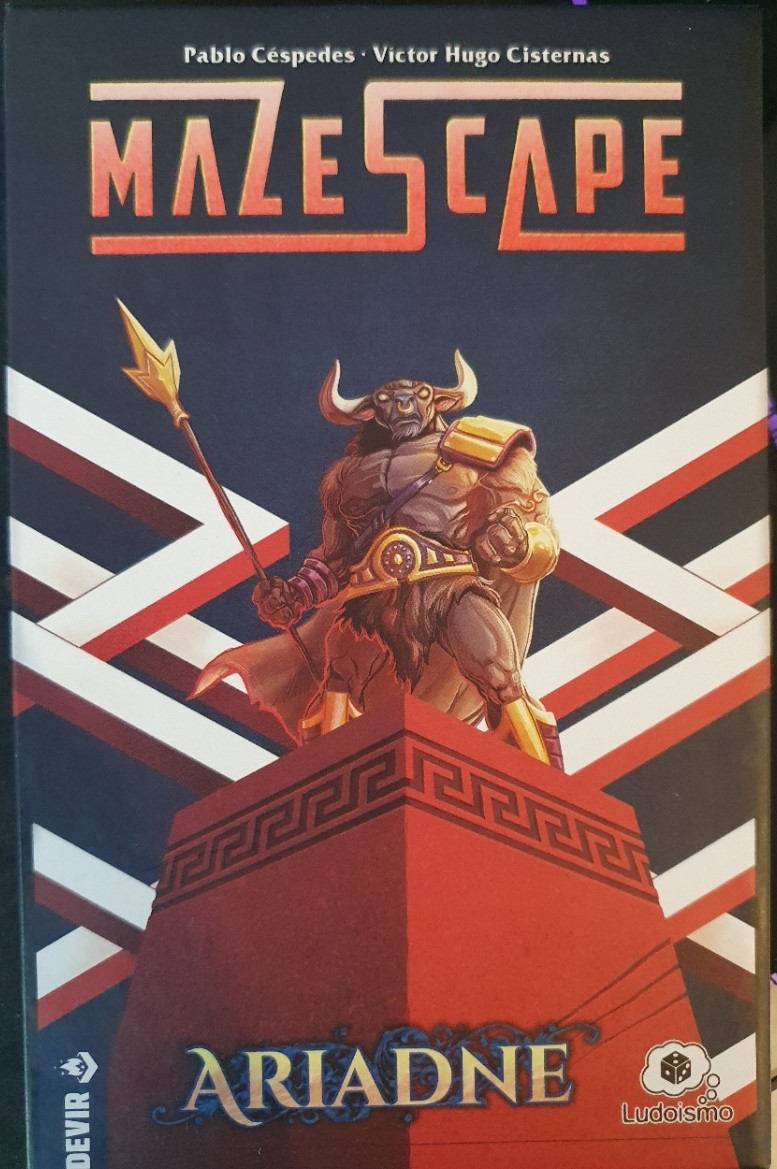
\includegraphics[width=1\linewidth]{content/pictures/MazeScape.jpg}
\caption{Verpackung des Spiels MazeScape (vgl. \cite{noauthor_mazescape_nodate})}
\label{fig:mazescape}
\end{figure}

\begin{figure}[ht]
\centering
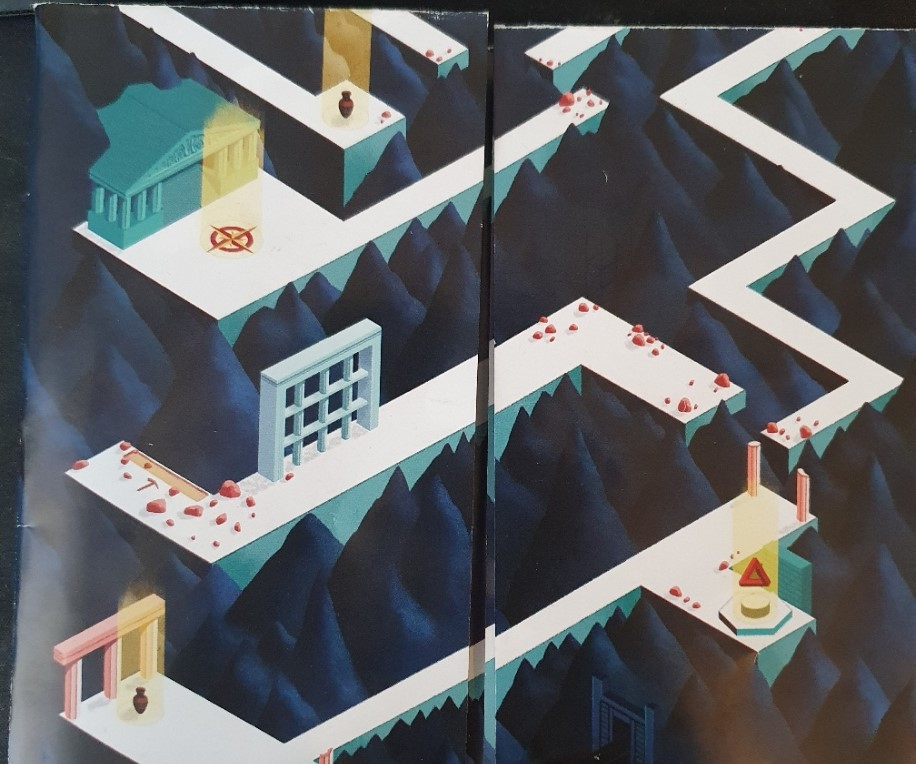
\includegraphics[width=1\linewidth]{content/pictures/MazeScape_Level02.jpg}
\caption{Level 02 aus dem Spiel MazeScape (vgl. \cite{noauthor_mazescape_nodate})}
\label{fig:mazescape_level-02}
\end{figure}

% Der Vortest umfasste das Spielen eines Levels aus dem Spiel MazeScape (vgl. Abbildung \ref{fig:mazescape}). Die Regeln wurden für den Anwendungszweck abgeändert. Die Probanden mussten zu zweit die 
Der Vortest umfasste das Spielen des zweiten Levels (vgl. Abbildung \ref{fig:mazescape_level-02}) aus dem Spiel \say{MazeScape} (vgl. Abbildung \ref{fig:mazescape}). Die grundlegenden Regeln des Spiels bezüglich der Bewegung durch die Spielwelt wurden für diesen Anwendungszweck übernommen. Die weiteren Regeln den Spiels zu bestimmten Gegenständen, Punkten oder Gegnern wurden aus dem Grund der fehlenden Relevanz nicht berücksichtigt. Die Probanden hatten zehn Minuten Zeit um gemeinsam vom Startpunkt im Level an das Ziel zu kommen. Es war dabei nicht wichtig rechtzeitig ans Ziel zu kommen.

Dieser Vortest wurde gemacht, damit ein Grundwert der bestehenden Kommunikation zwischen den Probanden zu bestimmen. Dieser sollte sich nach dem Nachtest verbessert haben.

Nach erfolgreich oder nicht erfolgreichem Abschluss des Vortests durften die Probanden den Prototyp von Connecting-Minds testen. Sie erhielten zunächst eine Einführung zur Steuerung der jeweiligen Anwendung. Anschließend durften sie starten. Sie hatten hierfür 40 Minuten Zeit. Ziel war es, die Rätsel zu lösen, allerdings war es nicht wichtig, ob sie das Tutorial erfolgreich in der gegebenen Zeit abschließen.

Die Zuordnung welcher Proband welche Spielrolle einnimmt, wurde nach der Begrüßung der Probanden vollzogen. Für die ersten Fragebögen war es wichtig zu wissen, wer welche Rolle im Spiel einnimmt. Daher erfolgt zum Ausfüllen der Einverständniserklärung die Einteilung von den Probanden ausgehend.

Nach absolvieren des Prototyps mussten die Probanden die Fragebögen zu den Themen System Usability, Immersion, Spiel Erfahrung Motivation und dem Workload des jeweiligen Probanden ausfüllen.

Im Anschluss folgte nun der Nachtest. Hierfür mussten die Probanden erneut ein Level aus dem Spiel MazeScape spielen. Sie spielten dabei das Level 3 (vgl. Abbildung \ref{fig:mazescape_level-03}). Wie im Vortest wurden die gleichen Regeln zur Bewegung durch die Spielwelt für den Versuch angewandt. Alle anderen Regeln wurden ebenfalls nicht berücksichtigt. Die Schwierigkeit, die sich in diesem Level für die Probanden ergeben hat, ist dass sie dass Ziel zunächst zusammen suchen müssen ehe sie einen Weg durch das Labyrinth finden können.

\begin{figure}[ht]
\centering
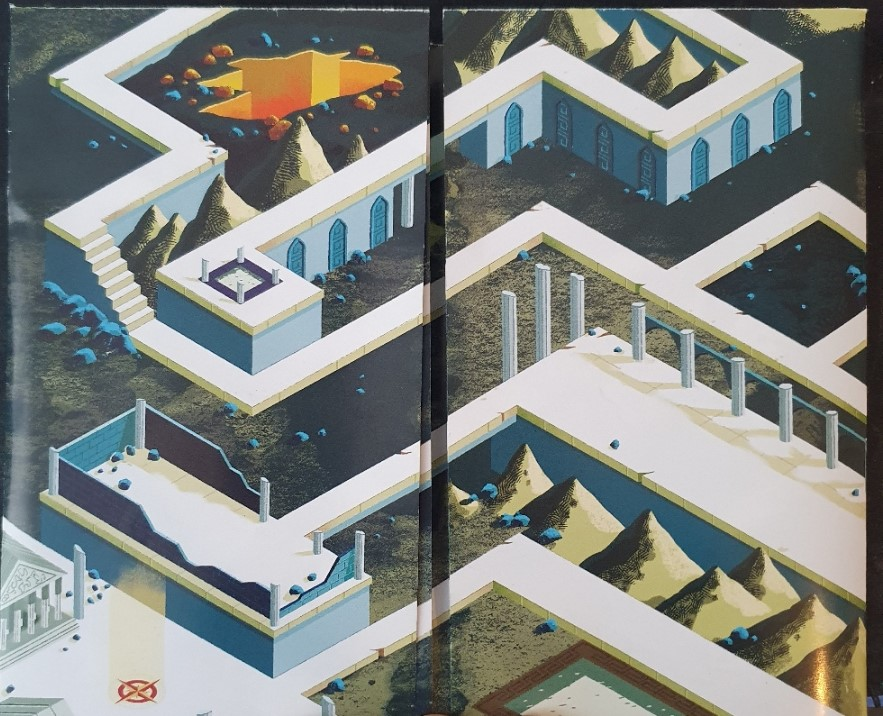
\includegraphics[width=1\linewidth]{content/pictures/MazeScape_Level03.jpg}
\caption{Level 03 aus dem Spiel MazeScape (vgl. \cite{noauthor_mazescape_nodate})}
\label{fig:mazescape_level-03}
\end{figure}

Wie im Vortest hatten die Probanden hierfür ebenfalls zehn Minuten Zeit. Außerdem war es ebenso nicht wichtig das Ziel zu erreichen.

Nach Abschluss wurden die letzten Fragebögen von den Probanden ausgefüllt. Sie behandelten Vergleichswerte im Bezug auf die gegenseitige Beziehung und dem affektiven Status. Außerdem mussten sie Fragebögen zum Thema Leadership und dem Umgang mit Menschen in diesem Versuchsaufbau ausfüllen. Zuletzt hatten sie noch ein Freitextfeld, bei dem ihr qualitatives Feedback zur Anwendung gegeben werden konnte.

Nachdem alle Fragebögen ausgefüllt wurden, wurde die Aufnahme beendet und es wurde sich bei den Probanden für die Teilnahme bedankt. Sie durften sich noch etwas von den bereitgestellten Snacks nehmen und wurden im Anschluss entlassen.

Die gesamte Versuchsdurchführung dauerte etwa 75 Minuten pro Probanden-paar.

\subsection{Rahmenbedingungen}
Für die Durchführung des Versuchsaufbaus wurde im I Bau der ehemaligen Fakultät Digitale Medien der Seminarraum reserviert. 

Da für das Durchführen der Probandentests einiges an Hardware benötigt wurde, wurde diese bei der Fakultäts-\ac{IT} und dem \ac{IIIUS}. Über die \ac{IT} wurden der Rechner, Bildschirm, Tastatur und Maus ausgeliehen, über welchen der Player seine Anwendung spielen konnte. Über das \ac{IIIUS} wurde das Google Pixel 7, ein Stativ und die Aufnahme Kamera von Sony ausgeliehen. Über das Smartphone konnte der Watcher seine Anwendung spielen. Die Kamera und das Stativ wurden gebraucht, um die Versuchsdurchführung aufzunehmen. Außerdem wurde bei Herrn Prof. Dr. Schnell ein TP-Link Router ausgeliehen, da sich die Anwendung des Players und des Watchers innerhalb des gleichen Netzwerkes befinden müssen um sich mit dem Server zu verbinden. Das Netzwerk der Hochschule verbietet es, dass sich Geräte innerhalb des Netzwerkes finden können.
Auf einem privaten Laptop liefen der Docker-Container der MongoDB und der Node-Server über den der WebSocket Server erzeugt wird. Außerdem wurde ein Wimaxit 15-Zoll Touchmonitor verwendet, über den der Player seinen Avatar durch die Spielwelt steuern konnte.

\begin{figure}[ht]
\centering
\includegraphics[width=1\linewidth]{content/pictures/Aufbau_00.jpg}
\caption{Versuchsaufbau des Experiments}
\label{fig:study-experiment-00}
\end{figure}

\begin{figure}[ht]
\centering
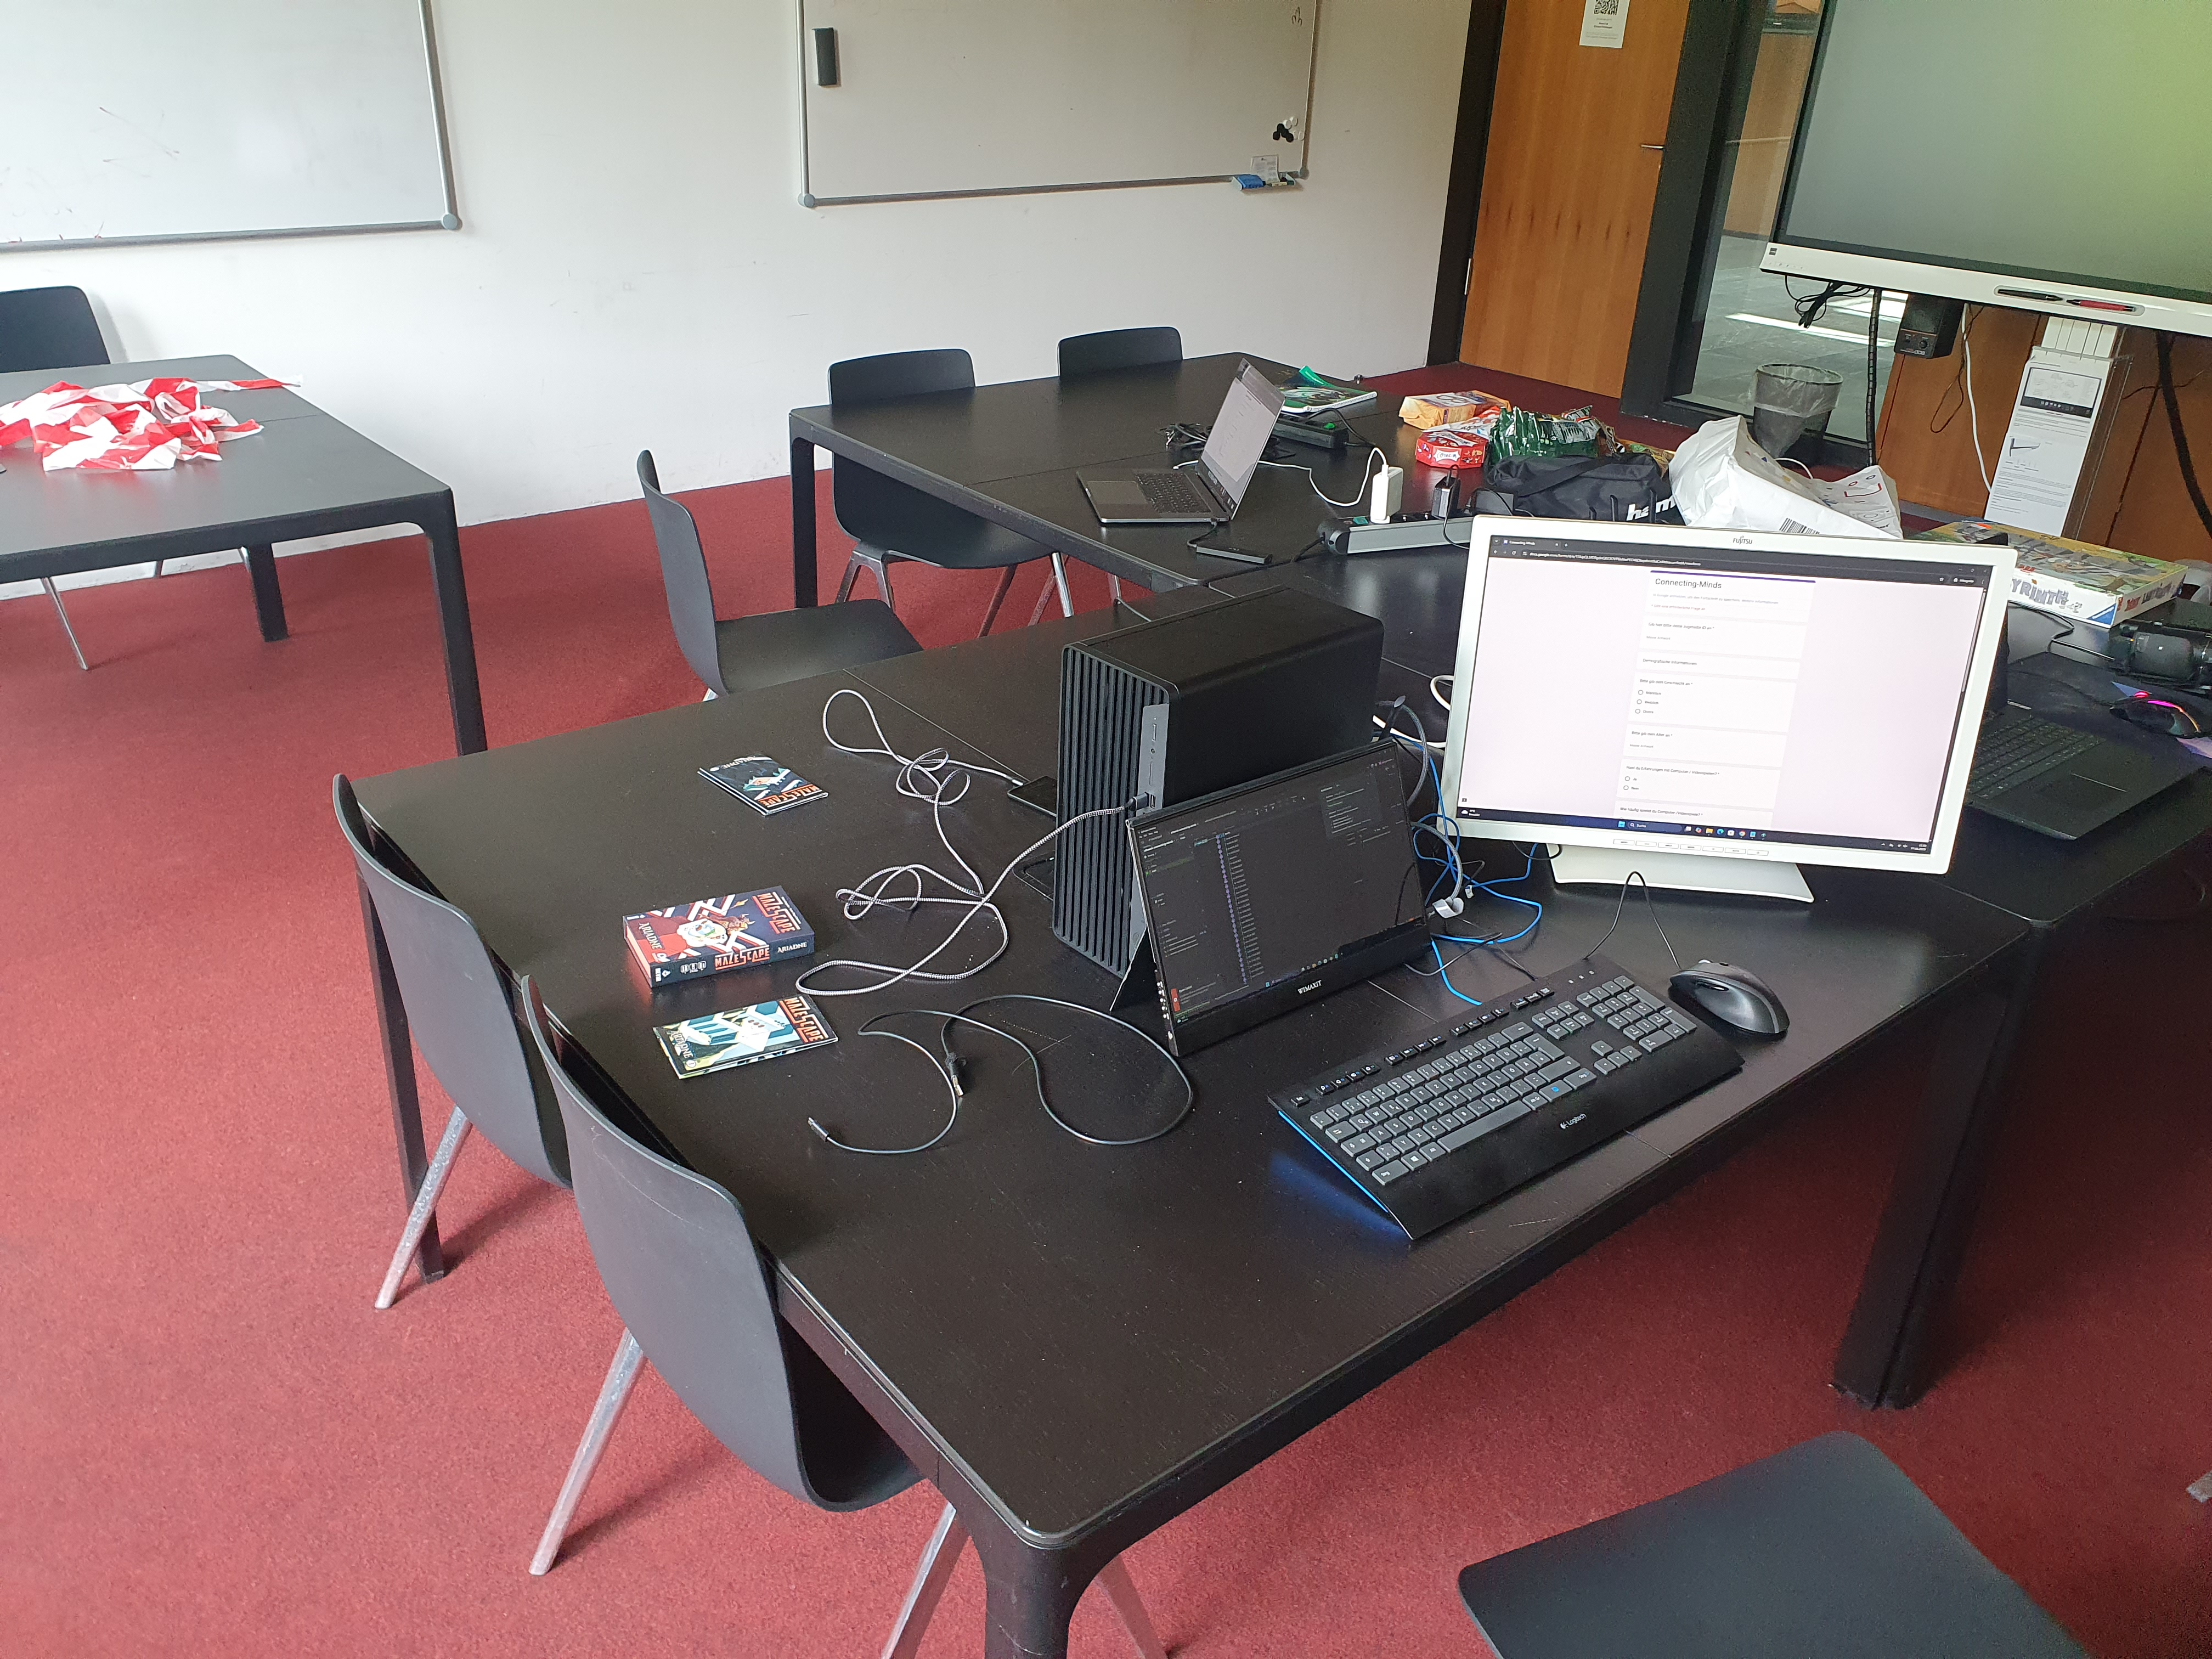
\includegraphics[width=1\linewidth]{content/pictures/Aufbau_01.jpg}
\caption{Versuchsaufbau Seite des Players}
\label{fig:study-experiment-01}
\end{figure}

\begin{figure}[ht]
\centering
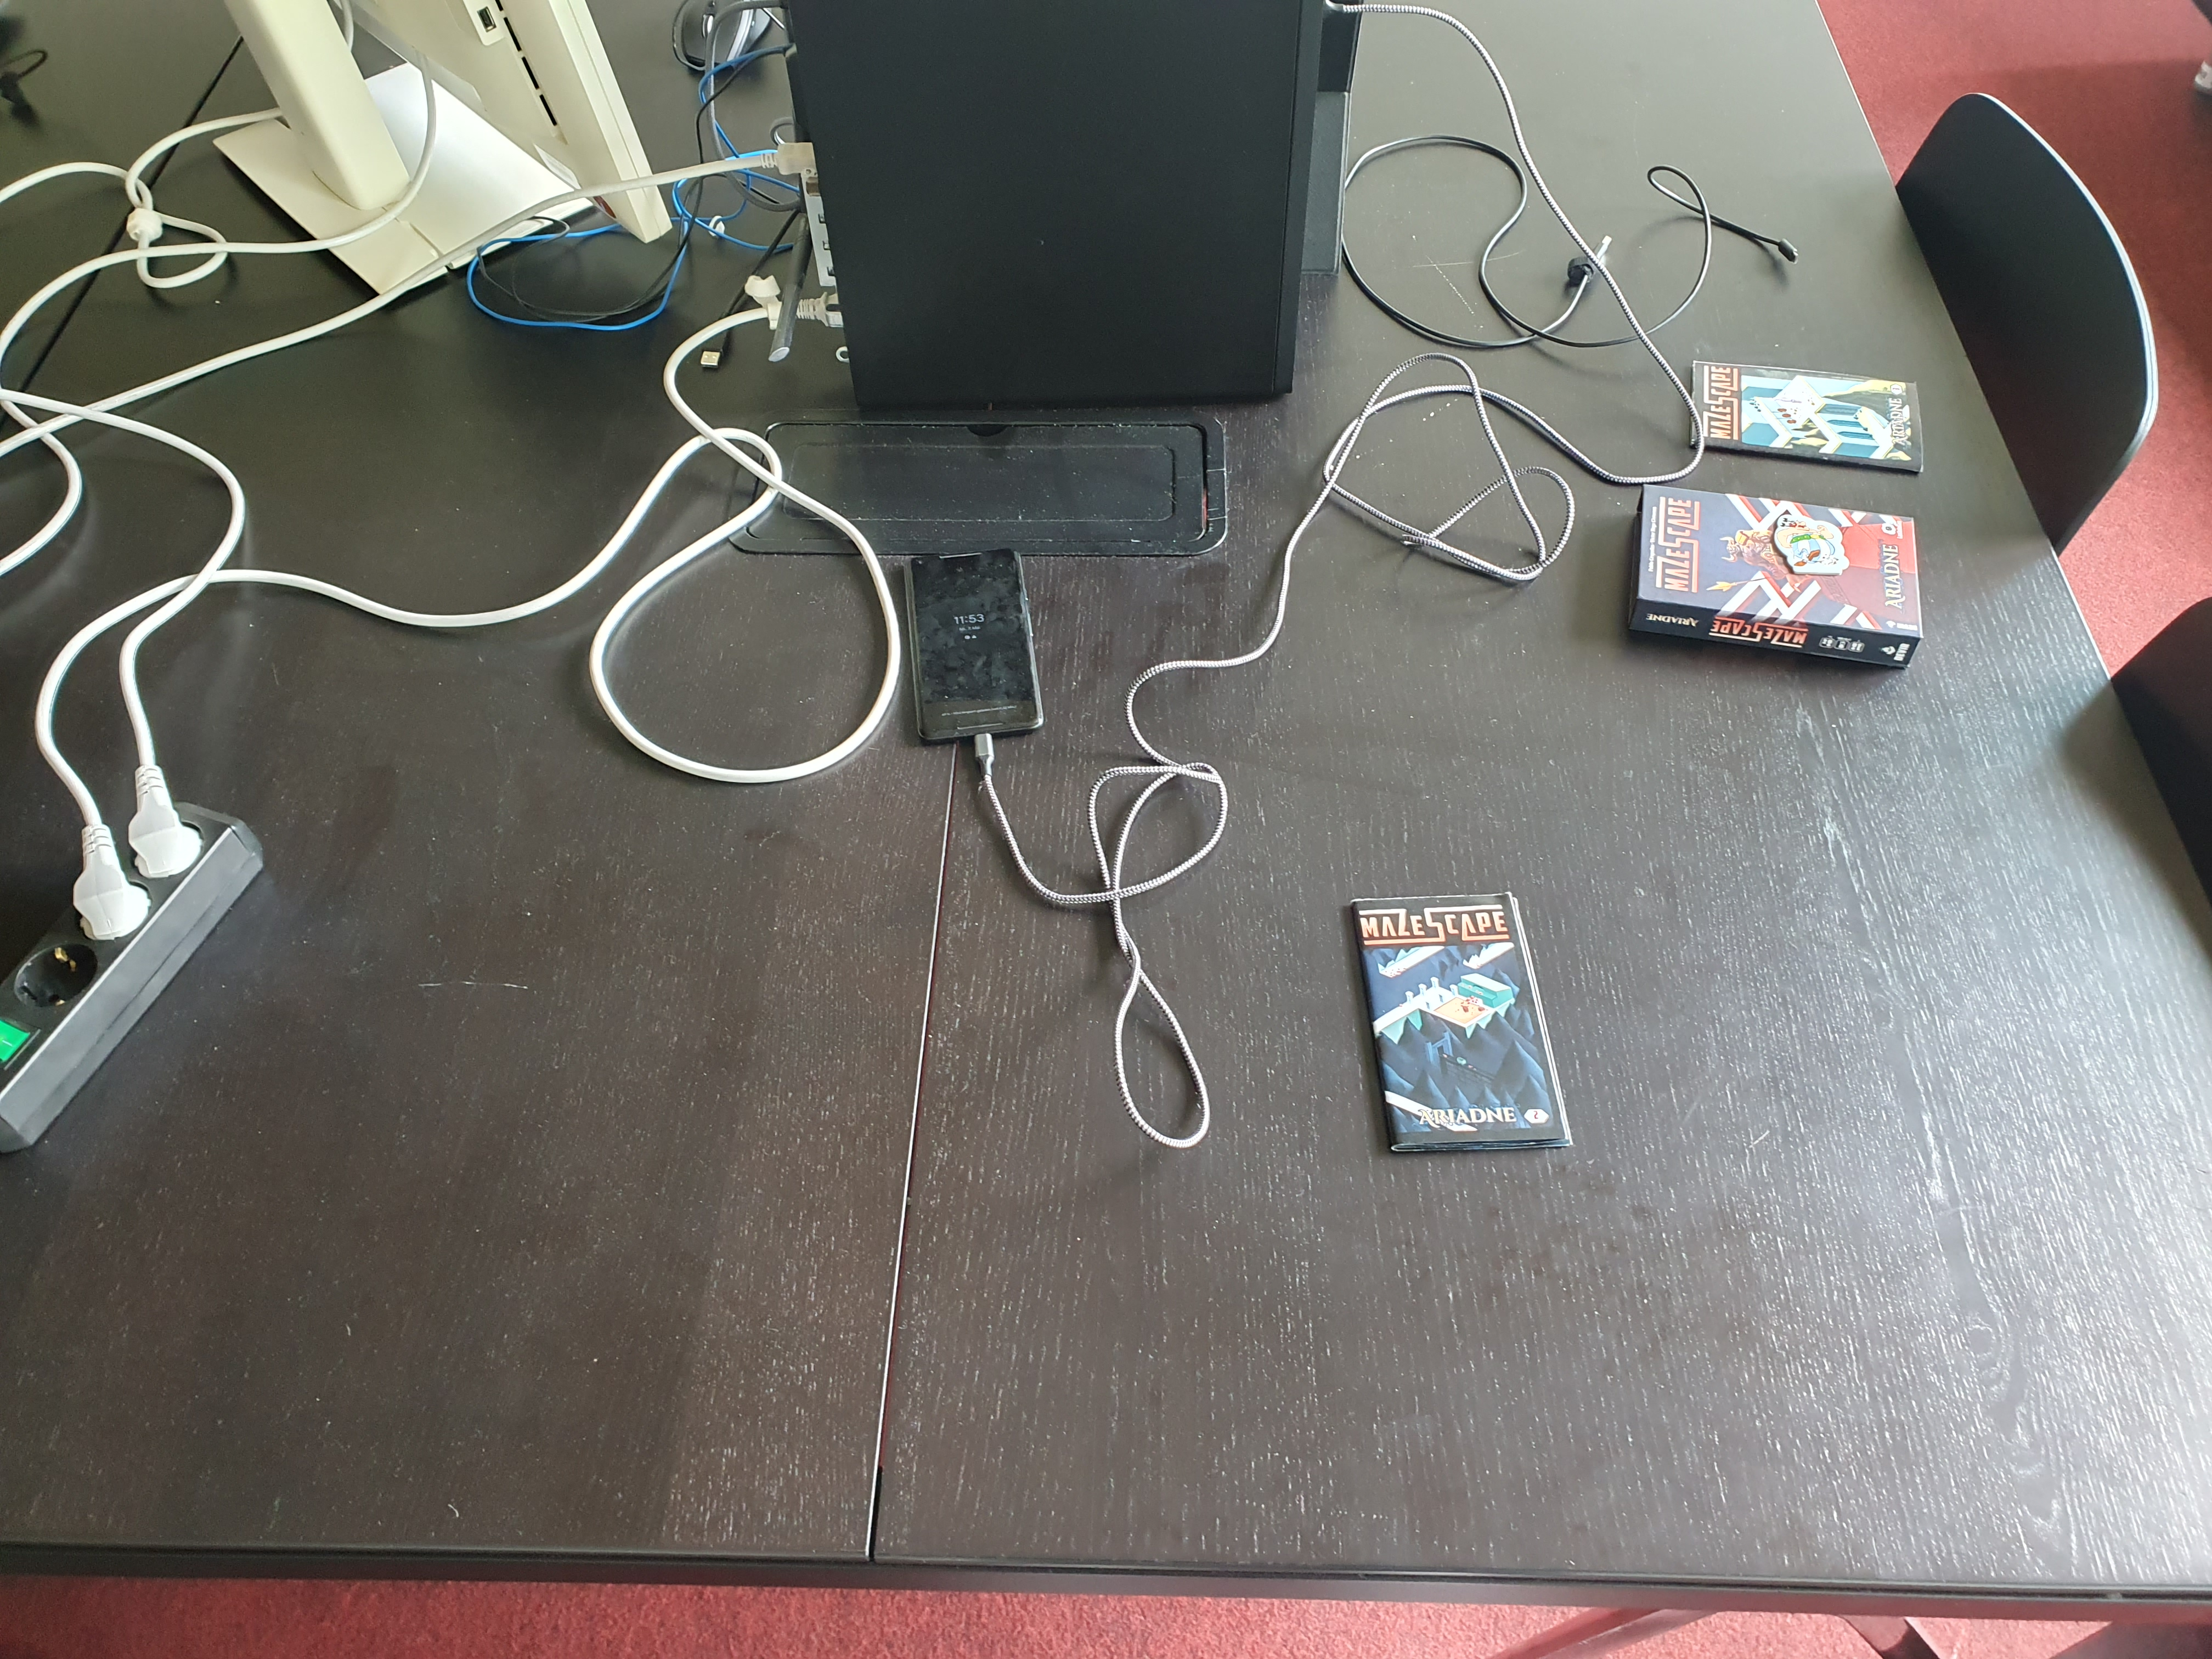
\includegraphics[width=1\linewidth]{content/pictures/Aufbau_02.jpg}
\caption{Versuchsaufbau Seite des Watchers}
\label{fig:study-experiment-02}
\end{figure}

Abbildung \ref{fig:study-experiment-00} zeigt wie der Seminarraum für die Versuchsdurchführung hergerichtet wurde. Beide Spielteilnehmer befinden sich jeweils gegenüber sitzend an einem quadratischen Tisch. Zwischen ihnen steht der Rechner der Player-Anwendung, damit sie physisch eine kleine Absperrung zwischen sich haben. Diese Absperrung ist grundlegend nicht relevant gewesen. So sollte vermieden werden, dass sich die beiden -Versuchsteilnehmer in die Anwendung des anderen schauen und so ggf. ohne den Einsatz der Kommunikation eine Lösung gefunden wird. Es war ihnen verboten in die Anwendung des anderen zu schauen.

Auf der rechten Seite des Tisches saß der Player (vgl. Abbildung \ref{fig:study-experiment-01}), der über den vor sich stehenden Touchmonitor seine Anwendung spielen konnte. Über den großen Bildschirm sollte er die Fragebögen der Versuchsdurchführung ausfüllen. Hierzu bekam der eine Tastatur und Maus. Der Watcher saß an der linken Seite des Tisches (vgl. Abbildung \ref{fig:study-experiment-02}). Hier konnte der Watcher über das beigelegte Google Pixel die Anwendung des Watchers spielen. Gespielt wurde die fertig gestellte \ac{3D}-Anwenung des Watchers. Außerdem sollten auf dieser Seite des Tisches die Probanden den Vor- und Nachtest des Versuches spielen. Dazu konnten sie sich entweder auf die Stühle setzen und durch das Labyrinth navigieren oder sie stellten sich hin.

Am hinteren linken Bildrand von Abbildung \ref{fig:study-experiment-00} steht ein weiterer Laptop, über welchen der Watcher seine Fragebögen ausfüllen musste.

\section{Ergebnisse}
In diesem Abschnitt werden die Ergebnisse der verschiedenen Fragebögen und der Aufzeichnungen der Versuchsdurchführungen vorgestellt.
Die Vorstellung erfolgt in drei Abschnitten. Zunächst werden die Ergebnisse der Demographischen Daten vorgestellt, im Anschluss erfolgt die Vorstellung der Ergebnisse bezüglich des Prototyps und zum Schluss werden die Kenntnisse aus den Aufnahmen vorgestellt.

\subsection{Vorstellung der demographischen Daten}
An der Versuchsdurchführung haben N=14 freiwillige Probanden (3 weibliche und 11 männliche; M = 25,86; SD = 4,52 Jahre) teilgenommen. Daraus ergeben sich für die Versuchsdurchführung 7-Zweierpaare. Zwei Probanden kannten sich zum Start der Versuchsdurchführung nicht, bzw. kannten sich nur vom Sehen. 12 der Probanden haben angegeben, dass sie bereits Erfahrungen mit Video- und Computerspielen gemacht haben, zwei hingeben haben bislang keine Erfahrungen gesammelt (fünf spielen mehr als 10 Stunden pro Woche, drei 6-10 Stunden, jeweils zwei spielen 3-5 und 1-2 Stunden pro Woche und zwei 0 Stunden die Woche. 13 von ihnen haben angegeben, dass sie bereits Erfahrungen mit Multiplayer-Spielen gesammelt haben, eine Person nicht (drei von ihnen spielen mehr als 10 Stunden Multiplayer-Spiele, einer 6-10 Stunden, vier 3-5 Stunden, fünf 1-2 Stunden und wieder eine Person 0 Stunden in der Woche). Insgesamt spielen 11 der Probanden kompetitive Multiplayer-Spiele, 10 kooperative, fünf kollaborative und eine Person andere Arten.
Auf die Frage nach Vorerfahrungen mit Spielen, die über eine Touchsteuerung gespielt werden, haben 13 \say{Ja} angeben, eine Person nein (eine Person spielt oft Spiele mit Touchsteuerung, drei Personen manchmal und  10 selten).

Die Abfrage bezüglich des Spielertyps ergab, dass sich sieben Teilnehmer des Typs Explorer, vier Teilnehmer des Typs Achiever, drei des Typs Killer und keiner des Typs Socializer zugehörig empfanden.

\subsection{Vorstellung der Prototyp-Evaluation}
Die Vorstellung der Fragebögen wird in die Dimensionen quantitative und qualitative Ergebnisse unterteilt.

In der quantitativen Auswertung der Fragebögen \ac{SUS}, \ac{GEQ}, \ac{IMI} und \ac{NASA-TLX} wurden zunächst für jeden Fragebogen bzw. dessen Subkategorien der \ac{M} und die \ac{SD} berechnet. Diese deskriptiven Kennwerte wurden für die Gesamtstichprobe (n = 14) sowie getrennt für die Gruppen \textit{Player} und \textit{Watcher} bestimmt, um mögliche Unterschiede zwischen den beiden Anwendungen zu identifizieren.

Zur Überprüfung signifikanter Gruppenunterschiede wurden die Daten in einem ersten Schritt auf Normalverteilung geprüft. Diese Prüfung erfolgte sowohl visuell anhand von \ac{Q-Q}-Diagrammen als auch mithilfe des Shapiro-Wilk-Tests. Diese Tests wurden jeweils separat für die Gruppen Player und Watcher durchgeführt. 

Je nach Ergebnis der Normalitätsprüfung kam für den anschließenden Gruppenvergleich ein unterschiedliches statistisches Verfahren zum Einsatz: Bei vorliegender Normalverteilung in beiden Gruppen wurde ein zweiseitiger t-Test für unabhängige Stichproben verwendet. Wenn mindestens eine Gruppe keine Normalverteilung aufwies, wurde stattdessen der Mann-Whitney-U-Test als nichtparametrische Alternative herangezogen.

Der folgende Abschnitt stellt nun die Ergebnisse dieser Auswertung für die einzelnen Fragebögen im Detail dar.
\paragraph{Quantitative Ergebnisse}
Der \ac{SUS} (Wertung zwischen 1: \say{stimme überhaupt nicht zu} und 5: \say{stimme voll und ganz zu}) ergab eine marginal hohe Usability (M = 69,11; SD = 13,64), wobei es starke Ausschläge nach oben (max = 92.5) und unten (min = 47.5) gibt. Damit eine Anwendung eine gute Usability haben kann muss sie mindestens einen Score von 73 haben (vgl. \cite[S. 36]{brooke_sus_2013}). In Bezug auf Unterschiede der Usability zwischen der Anwendungen des Watchers (M = 68,93; SD = 14,28) und des Players (M = 69,29; SD = 14,12) konnte über den t-Test (p = 0,95; t = 2,29) kein signifikanter Unterschied festgestellt werden.

Die Mittelwerte der einzelnen Kategorien des InGame Moduls des \ac{GEQ}s (Wertung zwischen 0: \say{überhaupt nicht} und 4: \say{extrem}) zeigen, dass die Probanden Spaß beim Spielen der Anwendungen hatten (Positive Emotionen: M = 3,07; SD = 0,83; Negative Emotionen: M = 0,54; SD = 0,75). Die Werte des Flows ( M = 3; SD = 0,94), Kompetenz (M = 2,54; SD = 0,89), Immersion (M = 2,54; SD = 0,89) und Herausforderung (M = 2,32; SD = 0,58) unterstützen dies, auch wenn sie nicht ganz so hoch bewertet wurden. Zwischen der Player und Watcher Anwendung beweisen der t-Test für Kompetenz (p = 0,19; t = 2,18), Flow (p = 0,42; t = 2,21) und Immersion (p = 0,60; t = 2,24) sowie der Mann-Whitney-U-Test für die restlichen Dimensionen keine signifikanten Unterschiede in den Bewertungen der einzelnen Komponenten (Anspannung: p = 0,65; U = 20,5; Herausforderung: p = 0,33; U = 17; negative Emotionen: p = 0,84; U = 22,5; positive Emotionen: p = 0,6; U = 20).

Die Mittelwerte des sozialen Präsenz Abschnittes des \ac{GEQ}s (Wertung zwischen 0: \say{überhaupt nicht} und 4: \say{extrem}) zeigen, dass die Teilnehmer gegenseitig Empathie verspürt (M = 3,11, SD = 0,55), wenig negative Gefühle gezeigt (M = 1,26; SD = 0,57) und verhaltensbezogene Beteiligung (M = 3,36; SD = 0,56) gezeigt haben. Auch hier gibt es keine Unterschiede in der Bewertung von Player und Watcher (Empathie: p = 0,855; U = 22.5; Negative Gefühle: p = 0,14; t = 2,19; Beteiligung: p = 0,45; t = 2,18).

Die Mittelwerte des Post-Game-Modul des \ac{GEQ}s (Wertung zwischen 0: \say{überhaupt nicht} und 4: \say{extrem}) zeigen, dass positive Erfahrungen (M = 2,38; SD = 0,88), wenn auch nicht so stark, aus dem Prototyp überbleiben, jedoch die Rückkehr in die Realität (M = 1,02; SD = 0,69) leicht fiel. Geringe Negative Erfahrungen (M = 0,31; SD = 0,31) zeigen, dass der durch die Usability entstandene Frust nicht überbleibt und die Probanden nicht ermüdet wurden (M = 0,68; SD = 0,82). In den Einzelkategorien der Positiven Erfahrungen (p = 0,56; t = 2.18), Negative Erfahrungen (p = 0,3: U = 16) und Müdigkeit (p = 0,88; t = 2,18) existiert kein signifikanter Unterschied zwischen den Anwendungen. Hingegen hat die Kategorie Rückkehr in die Realität (p = 0,04; U = 8.5) einen signifikanten Unterschied zwischen der Anwendung des Players und des Watchers. Der Mittelwert (M) der Watcher Anwendung wurde mit 1,43 höher bewertet als die des Players (0,62). Dieser Wert ist nicht hoch, allerdings hat die Anwendung des Watchers, vermutlich aufgrund ihrer Funktionen und der Führungsrolle im Design eine andere Wirkung, als die des Players.

Das Ergebnis des Abschnittes Interesse/ Vergnügen zeigt des \ac{IMI} (Wertung zwischen 1: \say{trifft überhaupt nicht zu} und 5: \say{trifft völlig zu}) zeigen, dass die Probanden überwiegend Interesse und Vergnügend zeigen konnten (M = 3,60; SD = 1,38). Zwischen der Bewertungen der Player und Watcher konnte kein signifikanter Unterschied festgestellt werden (p = 0,45; t = 2,21). 

Der \ac{NASA-TLX} zeigt (Basis Skala von 0 bis 10; skaliert auf 100er Skala), dass die Rätsel und die Steuerung eine höhere geistige Anstrengung (M = 63,57; SD = 14,47), eine sehr geringe körperliche Belastung (M = 4,29; SD = 6,46) und eine geringe zeitlich Anstrengung (M = 28,57; SD = 16,57) fordert. 
Der Prototyp konnte durchweg erfolgreich abgeschnitten werden, das zeigt der Leistungsteil (M = 75,14; SD = 17,85) des Fragebogens. Außerdem bot er eine durchwachsene Anstrengung (M = 50,71; SD = 19,79) und geringe Frustration (M = 29,29; SD = 31). Die umgesetzten Rätsel waren in ihrer Schwierigkeit nicht zu schwierig, boten allerdings dennoch eine Herausforderung. Die verbesserungswürdige Usability zeigt sich hier jedoch in der Frustration erneut. Zwischen der Anwendung des Players und Watchers konnten in den Unterkategorien (Geistige Anforderungen: p = 0,86; t = 2,22; Körperliche Anforderungen: p = 0,55; U = 29; Zeitliche Anforderungen: p = 0,76; t = 2,23; Leistung: p = 0,78; t = 2,21; Anstrengung: p = 0,9; t = 2,19; Frustration: p = 0,85; U: 26,5) keine signifikanten Unterschiede festgestellt werden.


Für die qualitative Auswertung des Freitextfeldes \say{Welches sonstige Feedback hast du?} aus dem allgemeinen Feedback zur Nutzerstudie und des Prototyps wurde sich an der thematischen Analyse von \cite{braun_using_2006} orientiert. Dabei wurde der sechs-stufige Prozess angewandt: Zunächst wird sich mit den Daten vertraut gemacht, danach werden erste Kategorien erstellt. Im Anschluss werden einzelne Themen gesucht, darauffolgend werden die Themen kontrolliert. Danach werden Themen definiert und benannt. Zum Schluss wird das Ergebnis präsentiert.

\paragraph{Qualitative Ergebnisse}
Abbildung \ref{fig:qualitative-results} zeigt, dass die Antworten aus dem Freitextfeld des Fragebogens in fünf Kategorien unterteilt werden können.
Unterteilt können die Ergebnisse in konstruktiver Kritik bezüglich der Anwendungen und allgemeinem positiven Feedback zum Spielkonzept und der Studie.
% Die Hauptthemen dabei sind die mangelhafte Steuerung, hauptsächlich die des Watchers, der Anwendungen 
Das Hauptthema der konstruktiven Kritik umfasst die verbesserungswürdige Steuerung, hauptsächlich die des Watchers, der Anwendungen. Zusammengefasst wurden jedoch das Rätsel und Environment-Design ebenfalls erwähnt.

% Im Kern wurde bei der Steuerung bemängelt, dass die manchmal umständlich, unintuitiv und unresponsiv ist. Weitere Aussagen beziehen sich dabei auf die Dreh- und Zoom Gesten der Watcher-Anwendung. Zudem wird vorgeschlagen diese in zwei Schritte aufzuteilen, damit sich diese nicht zu sehr überlagert. Vorgeschlagen wurde ebenfalls diese durch On-Screen Overlays zu ergänzen, um eine Unterteilung zwischen Zoom und Yaw zu erzielen. In Bezug auf die Steuerung des Players wurde darauf hingewiesen, dass die Veränderung der Sichtweise nach oben und unten in der First-Person-Ansicht nicht möglich und somit nur ein eingeschränktes Blickfeld vorhanden war. Außerdem gab es Schwierigkeiten in der Bewegung des Avatars, da teilweise kein Ziel ausgewählt werden konnte. 

\begin{figure}[ht]
\centering
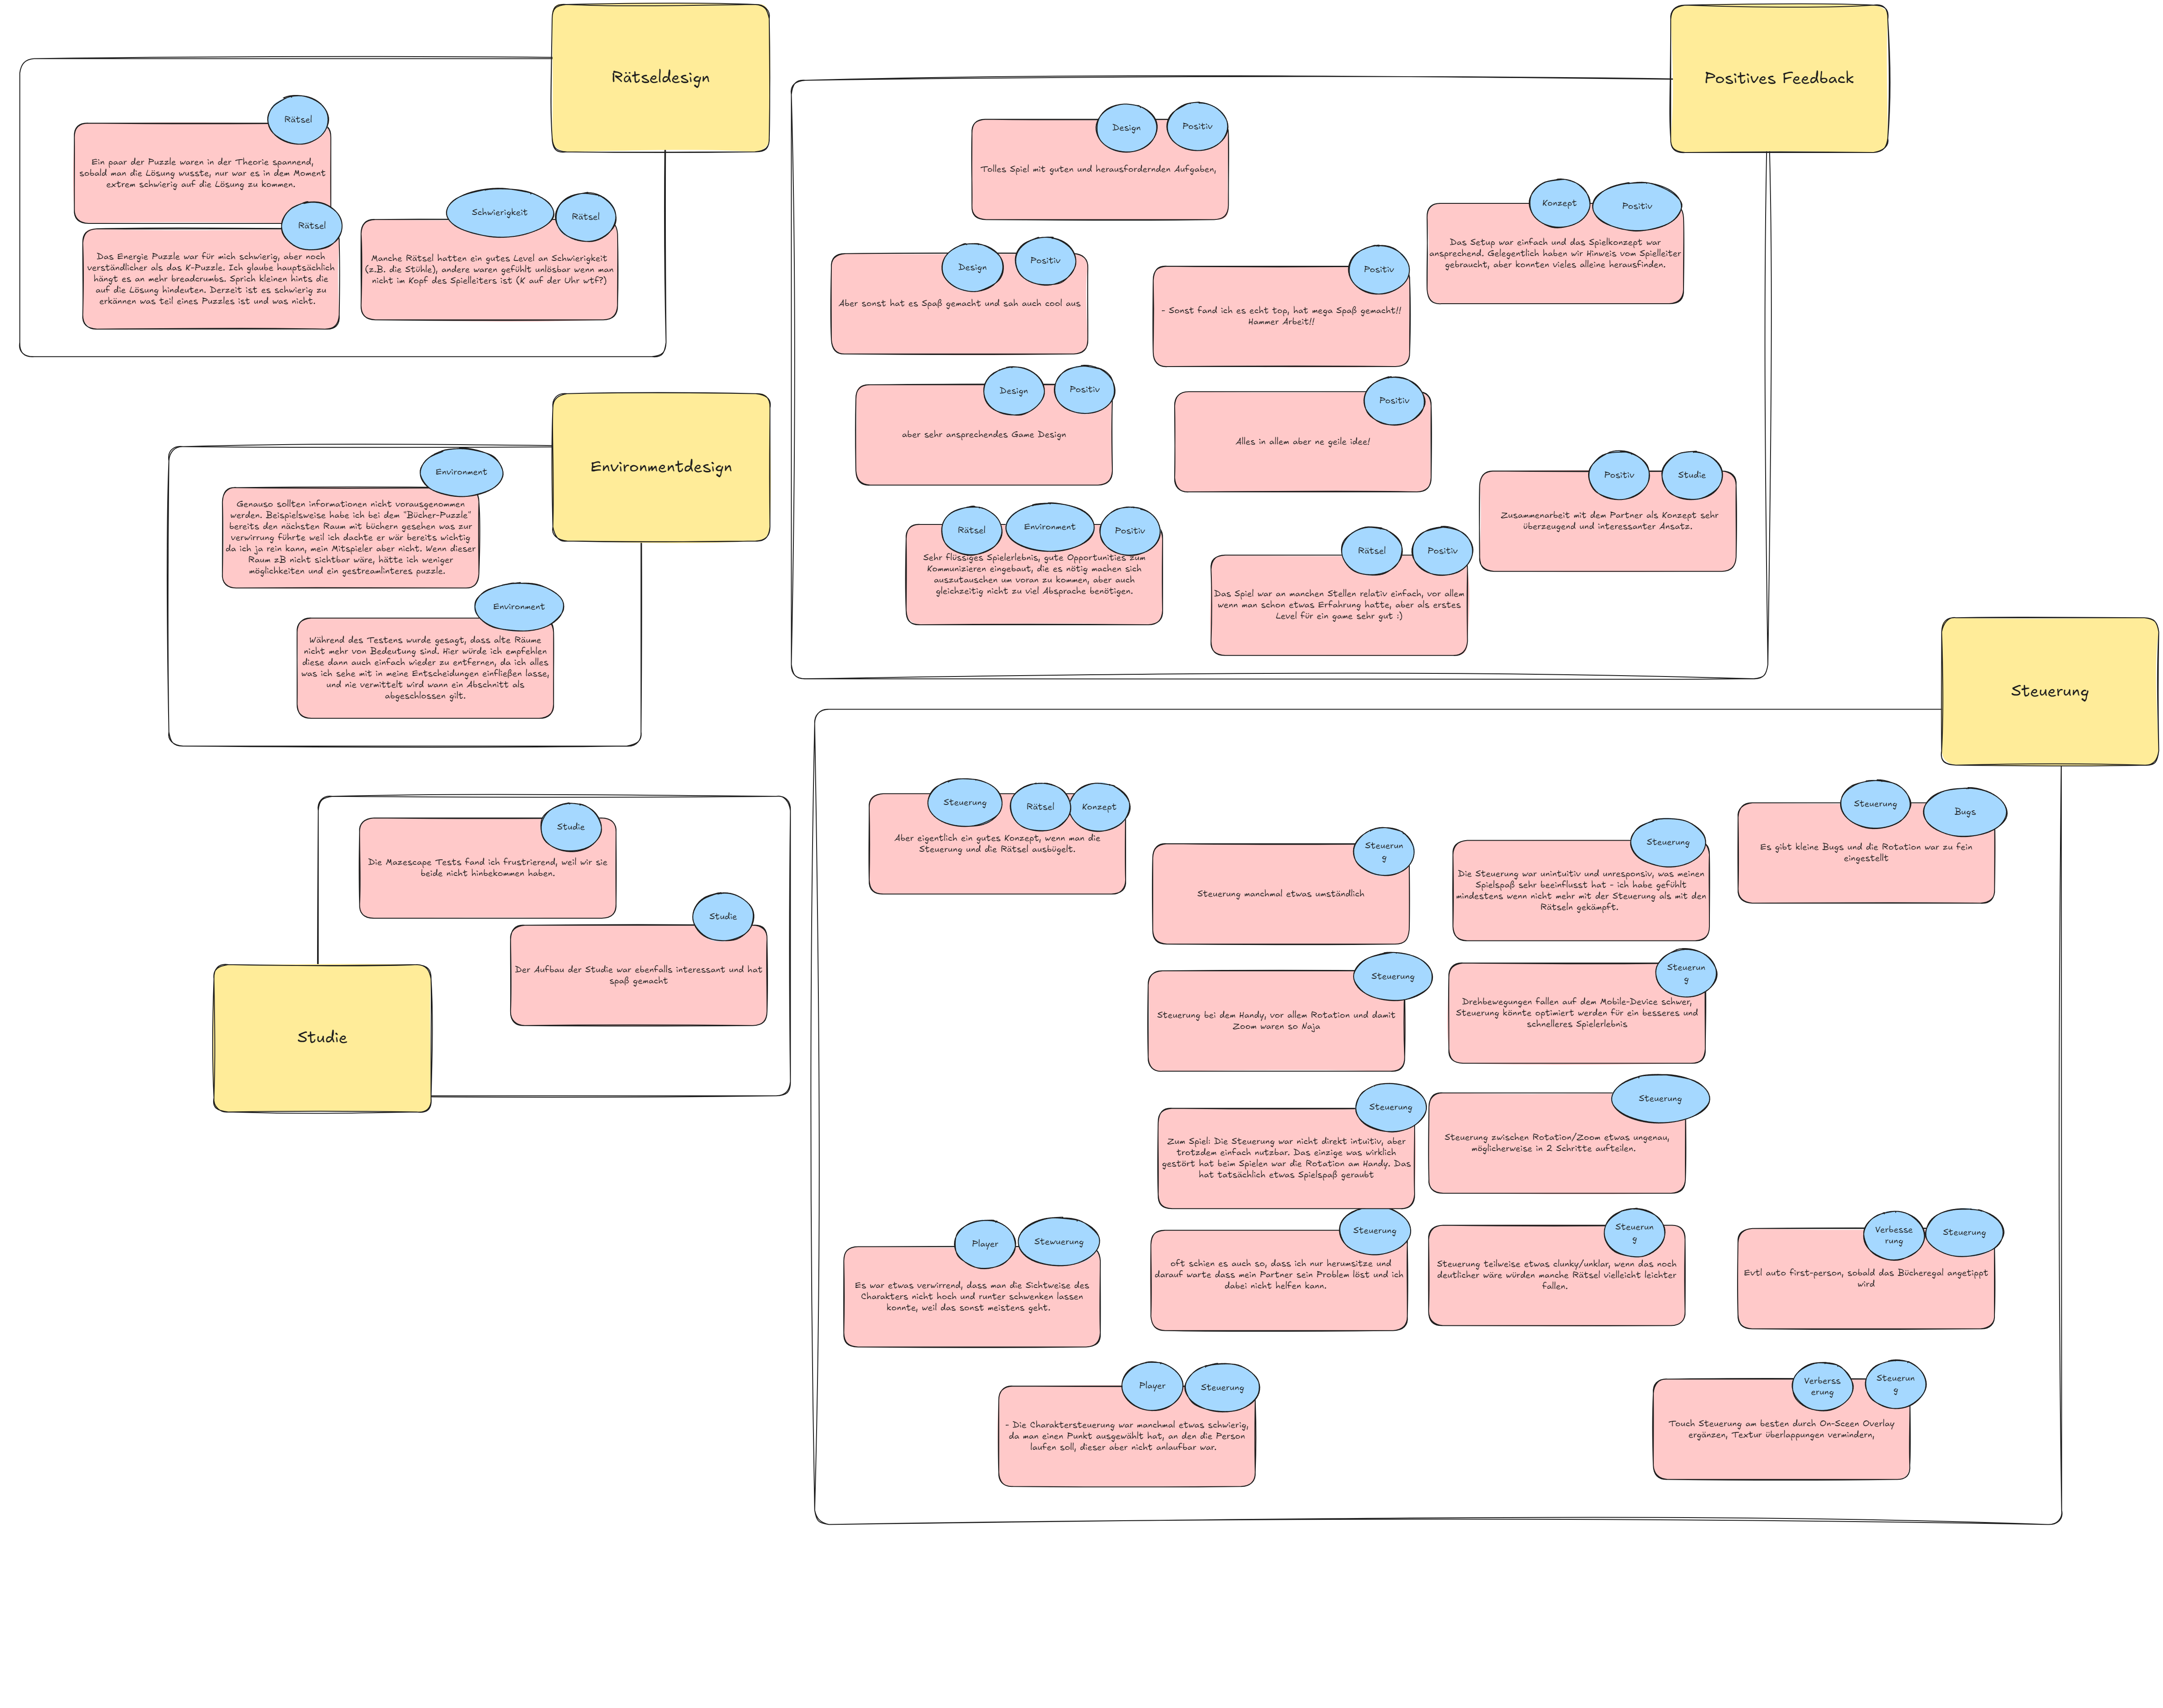
\includegraphics[width=1\linewidth]{content/pictures/Qualitative-Auswertung-Schritt-1.png}
\caption{Ergebnis der groben Kategorisierung nach \cite{braun_using_2006}}
\label{fig:qualitative-results}
\end{figure}

Abbildung \ref{fig:qualitative-results-end} zeigt die Zusammenführung des Feedbacks. 
Die Steuerung, vor allem die des Watchers, wird insgesamt als problematisch wahrgenommen. Mehrere Rückmeldungen beschreiben sie als umständlich, unintuitiv, unresponsiv oder \say{clunky} und unklar. Betroffen sind hierbei die Yaw- und Zoom - Geste der \ac{3D}-Anwendung. Mögliche Verbesserungsvorschläge, die benannt wurden, handelten von unterstützenden Elementen im Overlay-\ac{UI} des Spielers. So könnte eine bessere Unterscheidung zwischen dem Zoomen und dem Rotieren der Ansicht geschaffen werden. 
In der Player-Anwendung wurde das Fehlen einer vertikalen Bewegung der Kamera in der First-Person-Ansicht bemängelt, da momentan die Ansicht nur von einer vertikalen Perspektive aus genutzt werden kann. Zusätzlich gab es öfters Probleme damit, eine Zielposition auszuwählen, an die sich der Avatar bewegen soll.

In Bezug auf das Rätsel/ und Umgebungsdesign wurde bemängelt, dass teilweise die Lösungsfindung der Rätsel noch zu unausgereift und herausfordernd ist. 
Außerdem wird vorgeschlagen noch mehr Hinweise auf die Rätsel einzubauen, damit die Lösungsfindung einfacher gestaltet werden kann. Zudem wurde bemängelt, dass die Anzahl der aktiven Räume nach dem Lösen wieder deaktiviert werden können, damit diese das Lösen der neuen Rätsel nicht mehr behindern.

Die Nutzerstudio wurde als interessant und gut gemacht empfunden, allerdings bot der Vor- und Nachtest mit MazeScape Frustrationsgefahr.

Alles in allem bot der Prototyp Spaß am Spielen. Außerdem wurde das Spielkonzept von \say{Connecting-Minds} als ansprechend und überzeugend Umgesetzt angesehen. Gelobt wurde zudem das einfach Setup.
\begin{figure}[ht]
\centering
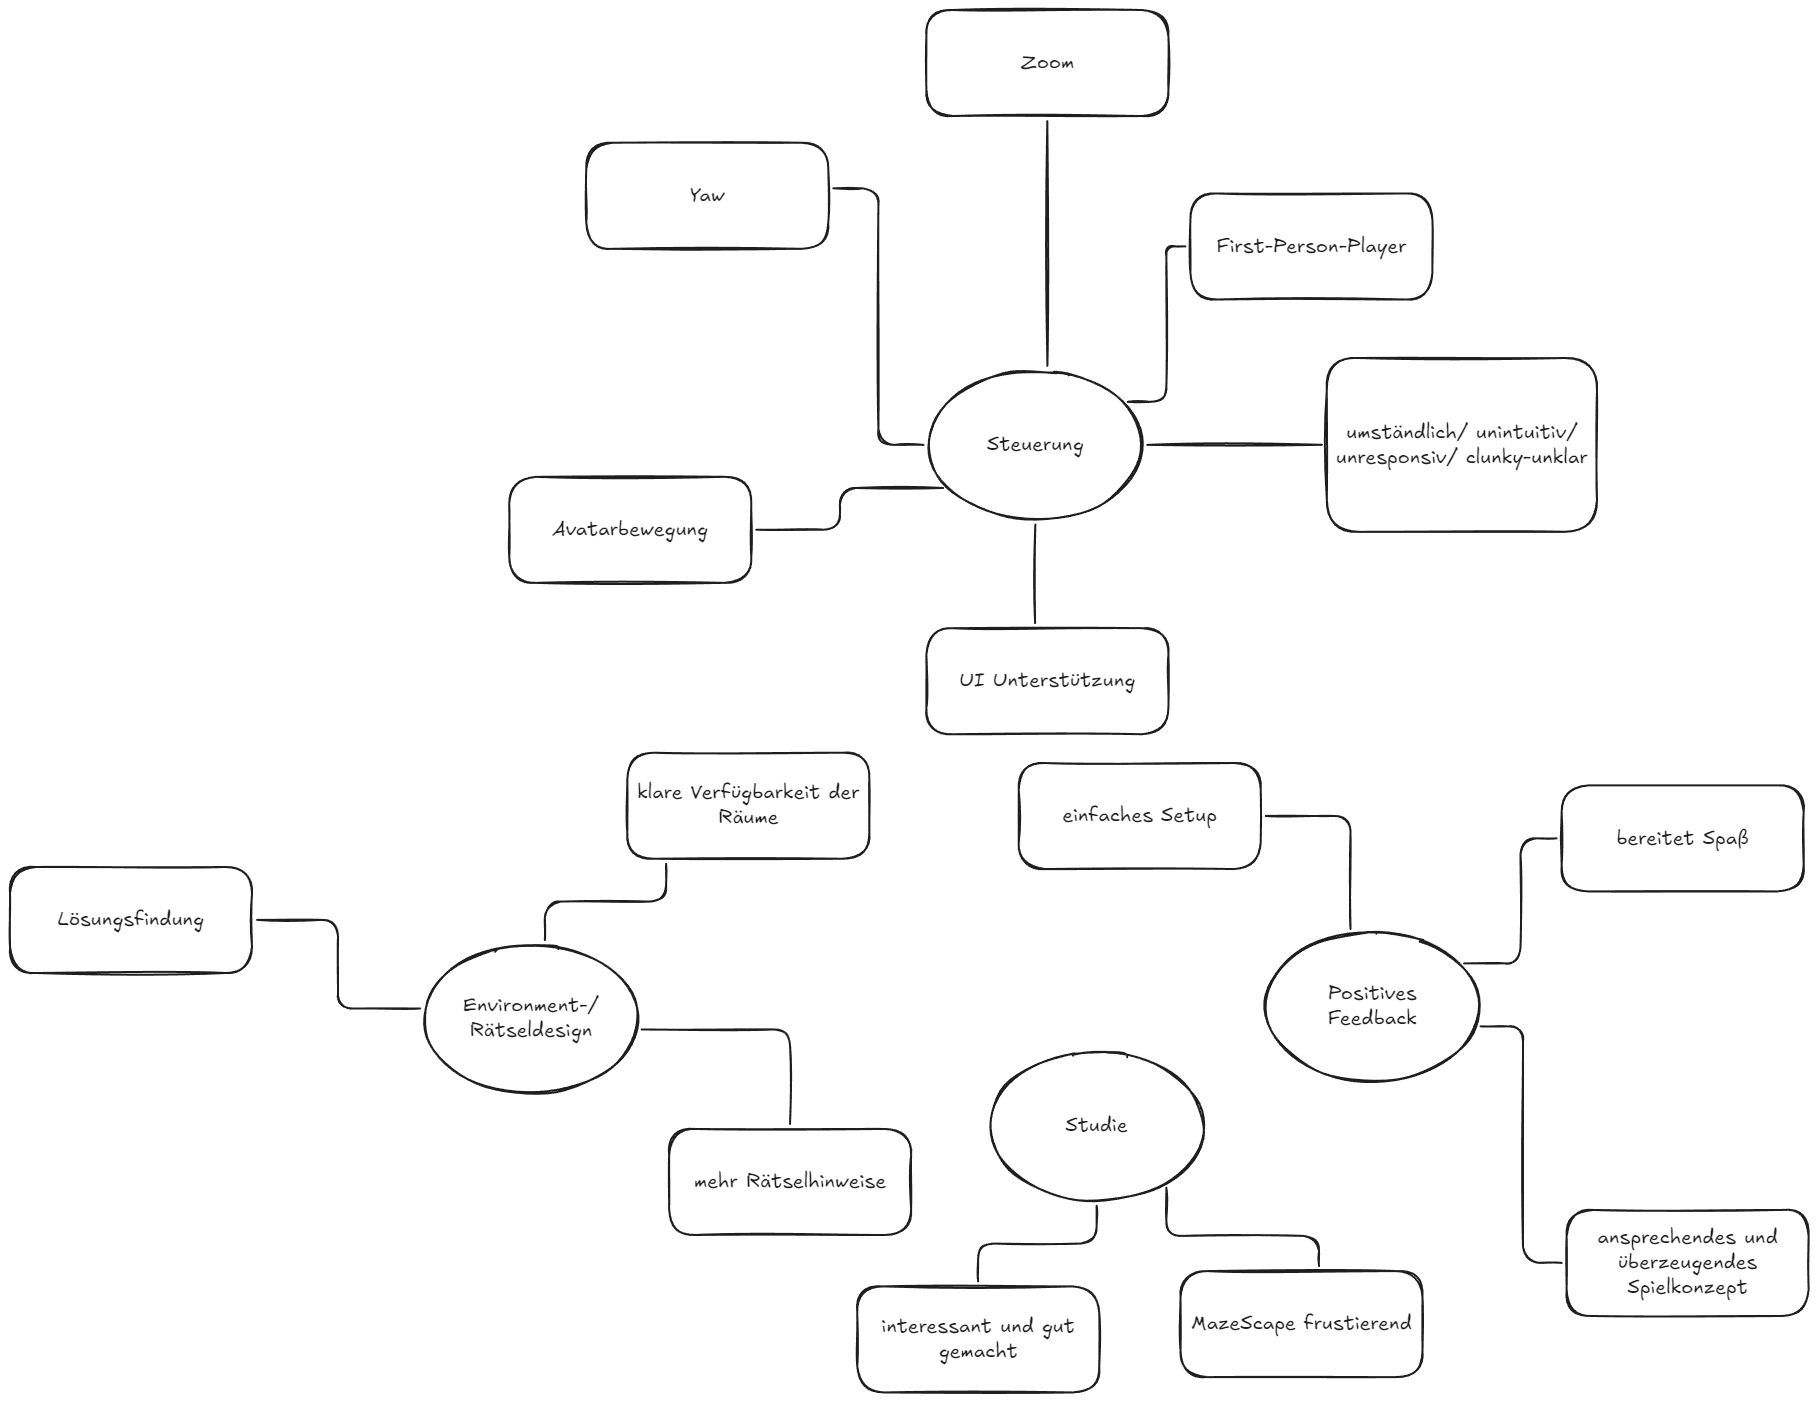
\includegraphics[width=1\linewidth]{content/pictures/Qualitative-Auswertung-Schritt-2.png}
\caption{Ergebnis der feinen Kategorisierung nach \cite{braun_using_2006}}
\label{fig:qualitative-results-end}
\end{figure}

% \paragraph{}

\subsection{Einordnung der qualitativen und quantitativen Ergebnisse}
Die Auswertung des Freitextfeldes zeigt genauere Ursachen bezüglich des niedrigen Wertes des \ac{SUS}'. Die niedrige Gebrauchstauglichkeit der  resultiert aus der fehlenden \say{Klarheit} und Verbesserungswürdigen Umsetzung der Steuerung der Anwendung des Watchers und des Players. Außerdem werden hier ebenfalls die angesprochenen Mängel des Rätsel- und Environmental-Designs berücksichtigt. Der allgemeine Durchschnitt der Frust-Skala aus dem \ac{NASA-TLX} kann hierbei nur bedingt als Unterstützung dienen. Der Mittelwert ist mit 29,29 nicht hoch, allerdings zeigt die Standabweichung von 31, dass bei einzelnen Probanden Frust erzeugt wurde. 

Die Ergebnisse des \ac{IMI}s und des \ac{GEQ}s zeigen, unterstützend durch das positive Feedback aus dem Freitextfeld, dass die Probanden trotz der genannten Schwierigkeiten Spaß und Freude entwickeln konnten.

\subsection{Vorstellung der Ergebnisse der subjektiven Wahrnehmung der Probanden}
% Die Wahrnehmung des \ac{IOS} und \ac{SAM}s wurden sowohl vor dem Vortest also auch nach dem Nachtest gemessen. Sie sollen
Im Folgenden werden die Ergebnisse zur subjektiven Wahrnehmung der Probanden im Hinblick auf den \ac{IOS} und den \ac{SAM} dargestellt. Die Einschätzungen wurden zu zwei Zeitpunkten erhoben; einmal vor dem Vortest als \say{Ground-Truth} und einmal nach dem Nachtest, um mögliche Veränderungen im Erleben sozialer Nähe und Affektivität im Verlauf des Experiments sichtbar zu machen.

\begin{figure}[ht]
\centering
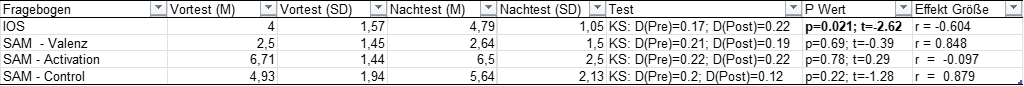
\includegraphics[width=1\linewidth]{content/pictures/IOS_SAM_Overal.png}
\caption{Ergebnisse des \ac{IOS} und \ac{SAM} auf alle Probanden bezogen}
\label{fig:ios_sam_overal}
\end{figure}

Abbildung \ref{fig:ios_sam_overal} zeigt die Ergebnisse des \ac{IOS}' und \ac{SAM}s. Der analysierte Datensatz umfasst sowohl die Antworten der Player als auch der Watcher. Eine Unterscheidung der Entwicklung in den einzelnen Rollen erfolgt im zweiten Schritt in Abbildung \ref{fig:ios_sam_roles}.

Zunächst wurden die Datensätze (der gesamte und seine Untergruppen) auf eine Normalverteilung überprüft. Dies erfolgte im gesamten Datensatz über den  Kolmogorov-Smirnov-Test. %(vgl. \cite{massey_kolmogorov-smirnov_1951}). 
Für die geteilten Datensätze wurden wie bei den Fragebögen zum Prototyp visuelle \ac{Q-Q}-Diagramme angelegt und anschließend über den Shapiro-Wilk-Test auf eine Normalverteilung untersucht.

Insofern die Datensätze vom Vor- und Nachtest in Normalverteilung vorlagen, wurde der t-Test für abhängige Stichproben durchgeführt, um zu bestimmen ob die vorliegende Änderung signifikant ist. Außerdem wurde die Effekt-Größe der Datensätze bestimmt. Für nicht-parametrische Datensätze wurde der Wilcoxon-Test für abhängige Stichproben angewandt.

Zusätzlich wurden die Untergruppen auf den Vergleich der Veränderungen untersucht, um feststellen zu können, welche Untergruppe eine stärkere Entwicklung vorlegen konnte. Für parametrisierte Untergruppen wurde der Welch-Test angewandt, für nicht-parametrisierte der Mann-Whitney-U-Test.

\paragraph{Allgemeine Auswertung}

Zunächst ist zu beobachten, dass die empfundene Nähe der jeweiligen Probanden-Paare, die über den \ac{IOS} gemessen wurde, im Mittelwert ansteigt. Diese Änderung ist signifikant und zeigt, dass zu den jeweiligen Testzeitpunkten die soziale Nähe der Probanden gestiegen ist. Es besteht hierbei eine mittlere Korrelation.

Die Valenz, also das Empfinden von positiver oder negativer Emotionen, (Wertung von 1 = glücklich bis 9 = unglücklich) steigt im Mittelwert leicht an. Außerdem steigt die Standardabweichung ebenfalls leicht an, wodurch die Einzelwerte der Stichprobe sich ein wenig gestreut haben. Dies kann durch Frustration in den jeweiligen Vor- und Nachtests oder der Usability des Prototyps verursacht worden sein. Die Änderung der Valenz ist jedoch nicht signifikant und zeigt eine sehr kleine Korrelation. 

Die Activation bzw. die Anspannung (Wertung von 1 = aufgeregt bis 9 = entspannt) der Teilnehmer stieg im Mittelwert ebenfalls leicht an. Die Probanden sind nach dem Test aufgeregter als zuvor. Jedoch zeigt die höhere Standardabweichung im Nachtest, dass die Eindrücke weiter verstreut liegen, als im Vortest.  Diese Änderung ist ebenfalls nicht signifikant. Sie zeigt auch eine sehr kleine negative Korrelation. Die entstandene Anspannung der Probanden kann durch die zeitlichen Begrenzungen, in welchen sie den Prototyp und die Vergleichstest durchführen müssen, erklärt werden. Außerdem kann der zuvor erlittene Erfolg oder Frust über das Lösen oder nicht Lösens des Nachtests ebenfalls eine Rolle spielen. 

Der Abschnitt des Controls, der Dominanz der Probanden, (Wertung von 1 = kontrolliert bis 9 = in Kontrolle) steigt ebenfalls an. Allerdings ist dies ebenfalls keine signifikante Änderung. Es konnte nur eine kleine Korrelation festgestellt werden. Die Wachsende Dominanz kann man dem wachsendem Selbstvertrauen, das die einzelnen Probanden im Verlauf des Experiments entwickeln konnten, zusammenhängen. Die Probanden lernen sich besser kennen und versuchen durch die Herausforderung der beiden Tests das Ziel zu erreichen.



\paragraph{Auswertung in der Unterscheidung zwischen Player und Watcher}

\begin{figure}[ht]
\centering
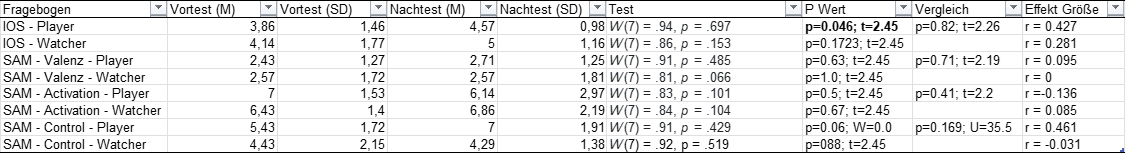
\includegraphics[width=1\linewidth]{content/pictures/IOS_SAM_Player_Watcher.png}
\caption{Ergebnisse des \ac{IOS} und \ac{SAM} auf beide Spielerrollen bezogen}
\label{fig:ios_sam_roles}
\end{figure}

Hierbei wurden nun der gesamte Datensatz in seine zwei Untergruppen, Player und Watcher, geteilt und getrennt ausgewertet. Es zeigt sich, dass der signifikante Unterschied in der Entwicklung der sozialen Nähe nur bei den Probanden der Player-Rolle signifikant ist. Ebenfalls ist bei der Player-Rolle die Korrelation höher, als bei der denen der Watcher. Allerdings konnte zwischen den Probanden der Player- und Watcher-Anwendung kein signifikanter Unterschied in der Veränderung festgestellt werden.

Wie im gesamte Datensatz bereits festgestellt wurde, kann auch in den Untergruppen kein signifikanter Unterschied in der Entwicklung der Valenz, Activation und Control festgestellt werden.

\subsection{Vorstellung der Ergebnisse der Quantisierung der Gesprächsflüsse}
In diesem Abschnitt werden die Ergebnisse der durchgeführten Vor- und Nachtests des Versuchsaufbaus vorgestellt. Die Tests wurden pro Probanden-Paar aufgenommen und mit Hilfe von \say{whisperx} (vgl. \cite{bain_whisperx_2023}) transkribiert. Die Arbeit von \cite{nasir_effect_2015} gab das Verfahren vor, auf welche Weise die Transkripte der Aufnahmen durchgearbeitet und analysiert werden mussten.

Zunächst wurden die Transkripte der einzelnen Tests in verschiedene Einzelblöcke unterteilt, welche entweder durch Pausen oder durch einen Wechsel im Gesprächsverlauf abgegrenzt. Eine Pause wurde wie bei Nasir als ein ununterbrochener Zeitraum von mehr als drei Sekunden, in dem keiner der Probanden spricht oder kein Gespräch führt, das über Interjektionen hinausgeht. Um innerhalb des Gesprächsablaufes einen qualitativen Wert entschlüsseln zu können, wurden die einzelnen Kommunikationsblöcke in sog. \say{Floor Holding}-Muster eingeteilt (vgl. \cite{edelsky_whos_1981}). \say{Floor Holding tritt auf, wenn eine bestimmte Person oder eine Gruppe von Personen den Gesprächsfluss für einen bestimmten Zeitraum dominiert.} \cite[S. 135, eigene Übersetzung]{nasir_effect_2015}. Unterschieden wurden in diesem Szenario wurden zwischen dem \say{\ac{CF}}, bei dem beide Probanden im Test miteinander zum Gesprächsfluss aktiv beeinflussen, und dem \say{\ac{SF}}, bei dem nur einer der beiden Probanden den Gesprächsfluss führt und der Partner bis auf Antworten oder Reaktionen auf das gesagte nichts zum Gespräch beiträgt.

Des weiteren wurden die Gesprächsblöcke zeitlich erfasst, wann diese im aufgezeichneten Video abgehalten wurden, damit festgehalten werden konnte, wie lange die Gespräche gingen und zu welchem Anteil sie im gesamten Test ausmachten. Sie wurden dabei im Verhältnis zur gesamten Arbeitszeit des einzelnen Test gewichtet. Wie in der Arbeit von Nasir wurden die einzelnen \say{Turns} gezählt, welche die einzelnen Beiträge der Teilnehmer darstellen. Zudem wurden die Wörter der einzelnen Abschnitte gezählt, um diese später als Vergleich für den gesamten Test zwischen den anderen Teilnehmern nutzen zu können. 

Zum Schluss wurden noch die gesagten Wörter der einzelnen Teilnehmer im ganzen Test gezählt und diese in Relation zur Gesamtmenge der gesagten Wörter gesetzt um den Gesprächsanteil dieses Probanden im Test ermitteln zu können.

Zusätzlich zu den Erhebungen von Nasir, wurde erfasst, welcher Teilnehmer wie oft die verschiedenen Gesprächsblöcke initiierte. Mit diesem Parameter soll die Entwicklung der Gesprächsinitiierung der Probanden bewertet werden.

Die jeweiligen Stichproben wurden mithilfe des Shapiro-Wilk-Test auf Normalverteilung geprüft. Anschließend wurden Veränderungen zwischen Vor- und Nachtest bei normalverteilten Stichproben mittels t-Test für abhängige Stichproben auf Signifikanz untersucht. Für nicht normalverteilte Stichproben kam der Wilcoxon-Test zum Einsatz. Zum Vergleich zweier unabhängiger Merkmale wurde der Welch-Test verwendet.

\begin{figure}[ht]
\centering
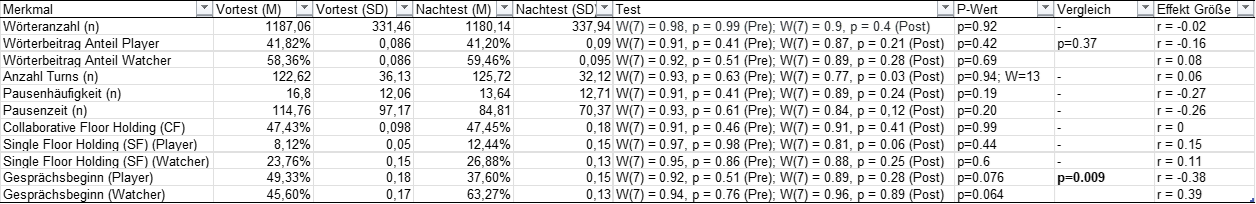
\includegraphics[width=1\linewidth]{content/pictures/quantitative_communication_results.png}
\caption{Ergebnisse des quantitativen Kommunikationsverhaltens aller Gruppen im Vergleich Vortest/Nachtest}
\caption*{\footnotesize Das Kürzel (n) bezeichnet normalisierte Werte auf 10 Minuten Gesprächsdauer.}
\label{fig:communication-results}
\end{figure}

Abbildung \ref{fig:communication-results} zeigt die Ergebnisse der quantitativen Untersuchung der einzelnen Probandentests. Abweichend von Nasir, der eine testweise Auswertung vornimmt, wurde hier pro Merkmal der durchschnittliche Wert aus allen sieben Tests für den Vor- und Nachtest verwendet.

Die einzelnen Gruppen erhielten für das kooperative Lösen der Labyrinth-Aufgabe 10 Minuten Zeit. Jedoch waren einige Gruppen früher fertig, manche wiederum wurden gar nicht fertig (M = 08:05 Minuten; SD = 02:27 Minuten Bearbeitungszeit im Vortest (M = 06:56 Minuten; SD = 03:15 Minuten Bearbeitungszeit im Nachtest). Aus diesem Grund wurden die in Abbildung \ref{fig:communication-results} betreffenden Merkmale normalisiert.

Die durchschnittlich gesprochene Wörteranzahl sinkt in der Entwicklung vom Vor- zum Nachtest leicht. Dieses negative Veränderung ist jedoch nicht signifikant und besitzt auch nur eine sehr kleine negative Korrelation. Außerdem stieg die bereits im Vortest hohe Standardabweichung ein Stück weiter an, wodurch eine größere Streuung der der Daten aus den Einzelgruppen sichtbar wird. 

Die Wörterbeiträge der Probanden aus den jeweiligen Gruppen des Players und Watchers wurden jeweils in ihren Tests im Verhältnis zu den gesamt gesprochenen Wörtern betrachtet. Der Mittelwert der Wortbeteiligungen der Player sank im Nachtest leicht, wohingegen die Wortbeteiligungen der Watcher leicht anstiegen. Beide Änderungen sind nicht Signifikant und besitzen auch nur eine geringe Korrelation. Die Anzahl der gemessenen \say{Turns} steigt jedoch leicht um ein nicht signifikantes Maß an.

Die Anzahl und die Länge der Pausen innerhalb des Gesprächsprotokolls reduzierten sich im Nachtest. In diesem Testszenario ist diese Veränderung zwar nicht signifikant, allerdings kann die mittlere negative Korrelation darauf hinweisen, dass in einem längeren Szenario Pausenzeiten signifikant reduziert werden könnten. Eine Reduktion der Anzahl und der Länge der Pausen kann zu einem positiven Kommunikationsverhalten führen.

Eine Analyse des Floor Holding Verhaltens der jeweiligen Probanden-Paare zeigt, dass das Kollaborative Verhalten im Mittelwert minimal ansteigt, jedoch in den \ac{SF}s der jeweiligen Teilnehmer im Vergleich stärker ansteigt. Alle drei Änderungen haben keine signifikante Verbesserung, auch eine niedrige Korrelation weißt nicht darauf hin, dass mit einem längeren Szenario und einer größeren Stichprobe am Wachstum eine Verbesserung messbar ist. 

Die Auswertung der Gesprächsstarts zeigte, dass die Probanden, die die Player Anwendung gespielt haben, im Nachtest seltener die Initiative ergriffen als noch im Vortest. Bei den Probanden der Watcher Anwendung ist es umgekehrt. Sie zeigten im Nachtest eine höhere Initiative und begannen öfters mit den Gesprächssequenzen. Beide Änderungen sind zwar nicht signifikant, besitzen aber beide eine mittlere Korrelation. Beim Vergleich der beiden Untergruppen konnte ein signifikanter Unterschied festgestellt werden. Bei einer größeren Stichprobe könnten die Entwicklungen der Initiativen signifikant werden.

In der gemeinsamen Gesprächsführung konnten sich die Probanden nicht verbessern, allerdings konnten sie häufiger von sich aus den Gesprächsfluss dominieren, wodurch ihr Selbstbewusstsein etwas zu sagen gestärkt werden konnte. Allerdings konnten in dieser Bewertungsform keine signifikanten Unterschiede festgestellt werden.


\subsection{Vorstellung der Ergebnisse zum Thema Leadership}
In diesem Abschnitt werden die Ergebnisse des Leadership-Fragebogens von \cite{emmerich_game_2016} in Bezug auf die Ergebnisse der quantitativen Auswertung der Vor- und Nachtests vorgestellt.

Zunächst wurden für jeden Probanden der Mittelwert der gewählten Werte berechnet (Wertung von 1 = trifft nicht zu; bis 5 = trifft vollkommen zu). Anschließend erfolgt die Gesamt-Durchschnittsberechnung. Die teilgenommenen Probanden zeigten insgesamt ein mittleres Maß an Führung (M = 3.92; SD = 1.18). 

Um die Mittelwerte der Player und Watcher Untergruppen miteinander vergleichen zu können, wurde zunächst durch den Shapiro-Wilk-Test auf Normalverteilung überprüft. Der Vergleich der Mittelwerte erfolgt über den ungepaarten t-Test.

Zwischen den Probanden der Watcher-Gruppe (M = 3.06; SD = 1.24) und der Player-Gruppe (M = 2.99; SD = 1.14) konnte kein signifikanter Unterschied festgestellt werden (p = 0.71; t = 2.18). 

Im Anschluss wurde untersucht, ob das Leadership Verhalten der einzelnen Probanden eine mögliche Korrelation mit ihren gesprochenen Worten im Nachtest besteht. Dafür wurde der Spearman'sche Rangkorrelationskoeffizient verwendet.

\begin{figure}[ht]
\centering
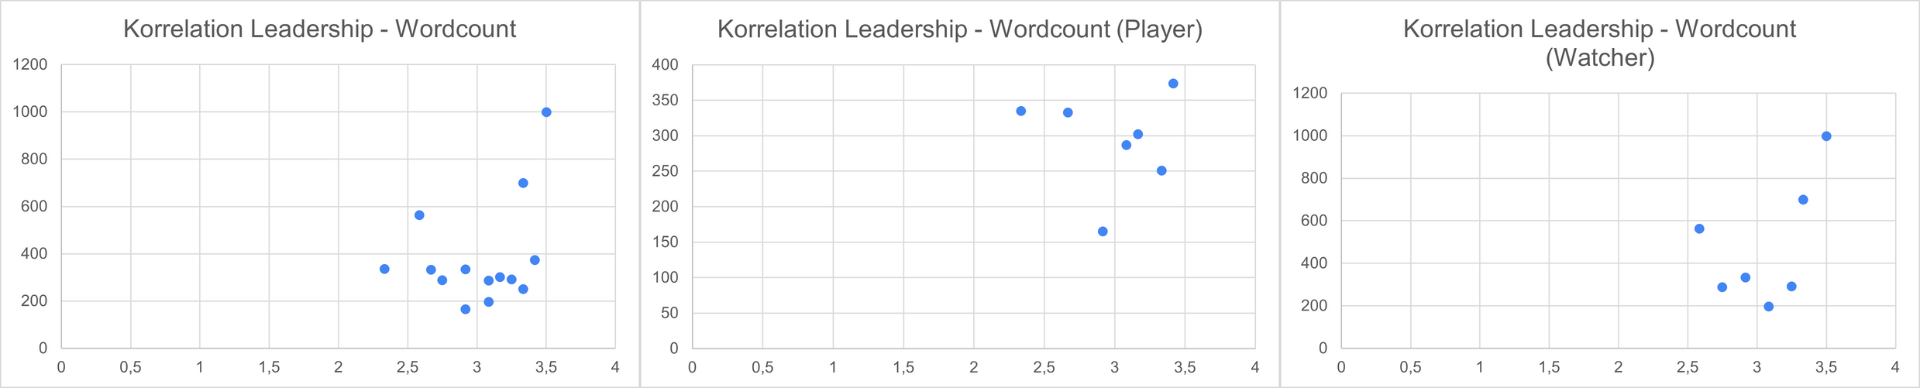
\includegraphics[width=1\linewidth]{content/pictures/Korrelation_Leadership_Wordcount_full.png}
\caption{Korrelation des Leaderships mit den gesprochenen Worten aus der quantitativen Gesprächsauswertung}
\label{fig:correlation_leadership_wordcount}
\end{figure}

In Betrachtung aller Probanden mit ihrem durchschnittlichen Leadership-Wert konnte nur eine sehr schwache Korrelation und keine Signifikanz festgestellt werden (rs(14) = 0.13; p = 0.66) (vgl. Abbildung \ref{fig:correlation_leadership_wordcount}, linkes Schaubild). In der Untergruppe der Watcher (vgl. Abbildung \ref{fig:correlation_leadership_wordcount}, rechtes Schaubild) konnte eine mittlere Korrelation festgestellt, welche ebenfalls nicht signifikant ist (rs(7) = 0.46; p = 0.29). In der Untergruppe der Player konnte keine Korrelation festgestellt werden (vgl. Abbildung \ref{fig:correlation_leadership_wordcount}, mittleres Schaubild). Diese ist ebenfalls nicht signifikant (rs(7) = 0; p = 1)

Da in dieser Arbeit eine verbesserte Kommunikation zwischen den Probanden angestrebt wird, steht insbesondere die Förderung kollaborativer Kommunikationsanteile im Fokus. Wie in der quantitativen Auswertung bereits festgestellt werden konnte, gab es keine signifikante Änderung in den Anteilen des \ac{CF}s. Da die Mittelwerte der Leadership-Selbsteinschätzung im mittleren Bereich liegen, lässt sich vermuten, dass keiner der teilnehmenden Personen eine dominante Führungsrolle einnimmt. Stattdessen könnte dies auf ein grundsätzlich kooperatives Miteinander hinweisen, in dem Führungsaspekte gleichmäßig verteilt und kollaborative Kommunikationsformen bevorzugt werden.

Dafür wurden nun Durchschnitte der Leadership-Werte der Probanden genommen, die an den Tests gemeinsam teilgenommen haben, und diese werden nun mit den Einzelwerten der \ac{CF}s der eigenen Tests verglichen.

\begin{figure}[ht]
\centering
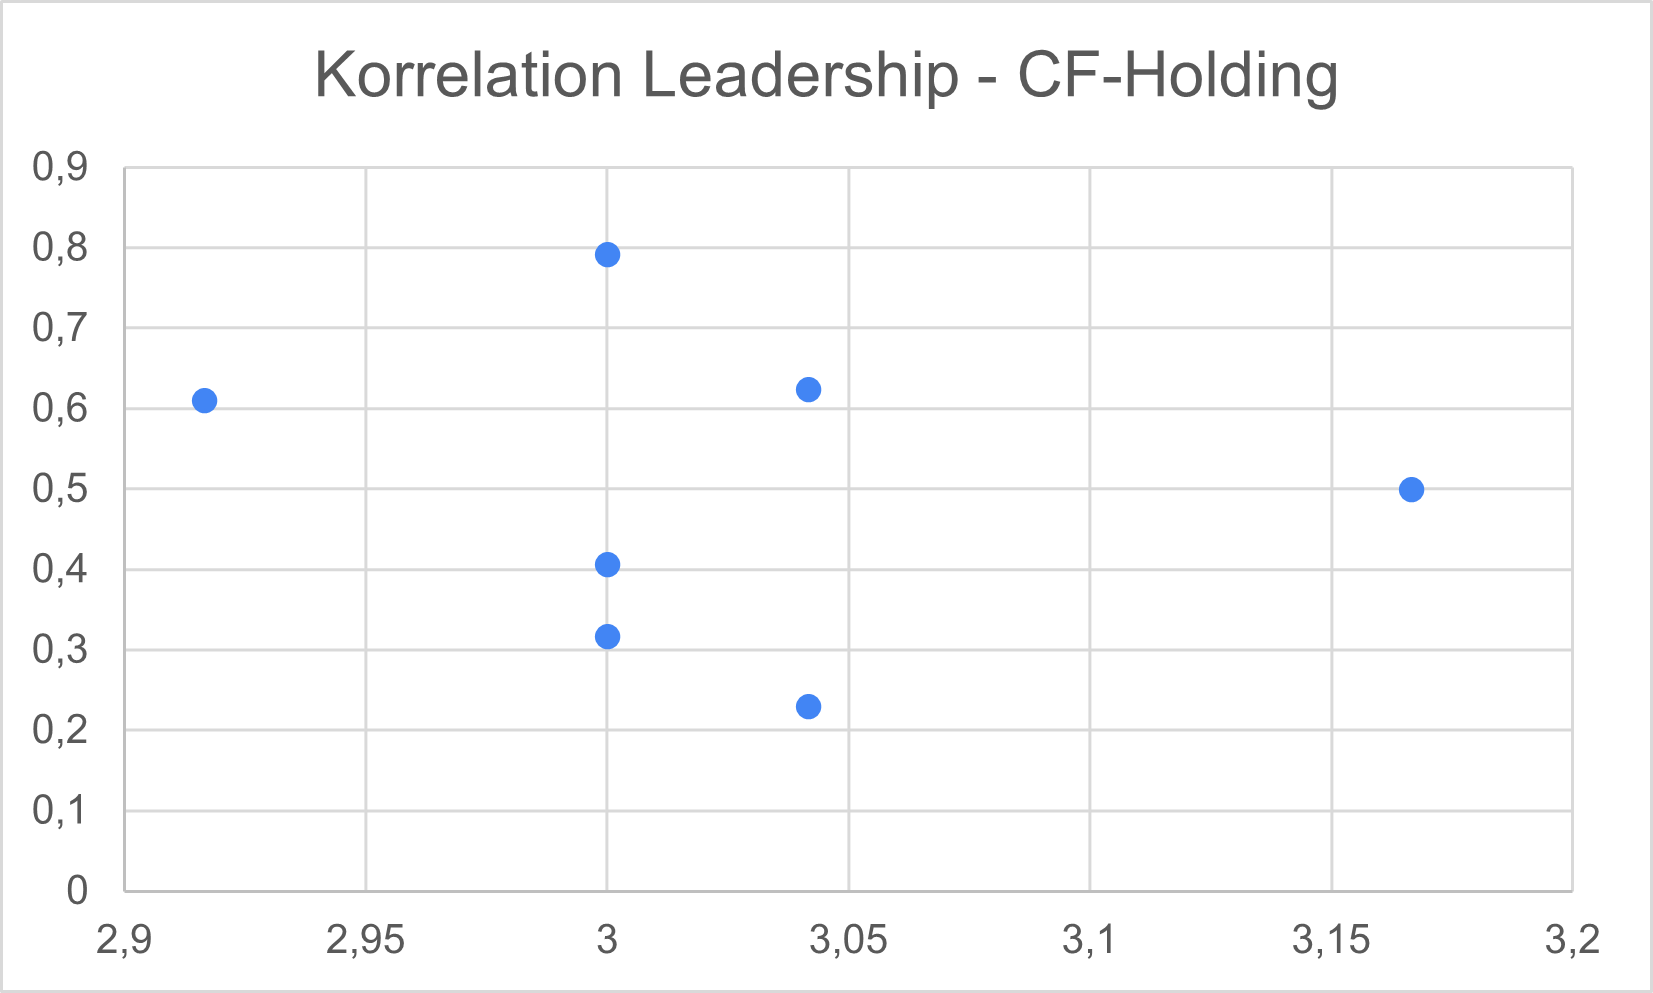
\includegraphics[width=1\linewidth]{content/pictures/korrelation_leadership_cfh.png}
\caption{Korrelation des Leaderships pro Probanden-Paar mit dem \ac{CF}-Anteil ihres Nachtests}
\label{fig:correlation_leadership_cfh}
\end{figure}

Es konnte keine Korrelation (vgl. Abbildung \ref{fig:correlation_leadership_cfh}) zwischen dem durchschnittlichen subjektiven Leadership Empfinden der Probanden-Paare mit ihrem \ac{CF}-Anteil in ihren jeweiligen Nachtests festgestellt werden. Diese hat außerdem keine Signifikanz (rs(7) = -0.08; p = 0.86).

Zuletzt wurde noch das subjektive Empfinden des Leaderships mit den gemessenen Anteilen der Gesprächsstarts untersucht (vgl. Abbildung \ref{fig:correlation_leadership_conversation_starts}). Auch hier zeigten sich weder in der Gruppe der Player (rs(7) = -0.07; p = 0.88), noch in der Gruppe der Watcher (rs(7) = -0.03; p = 0.94) Korrelationen, die ebenfalls nicht signifikant sind. 

\begin{figure}[ht]
\centering
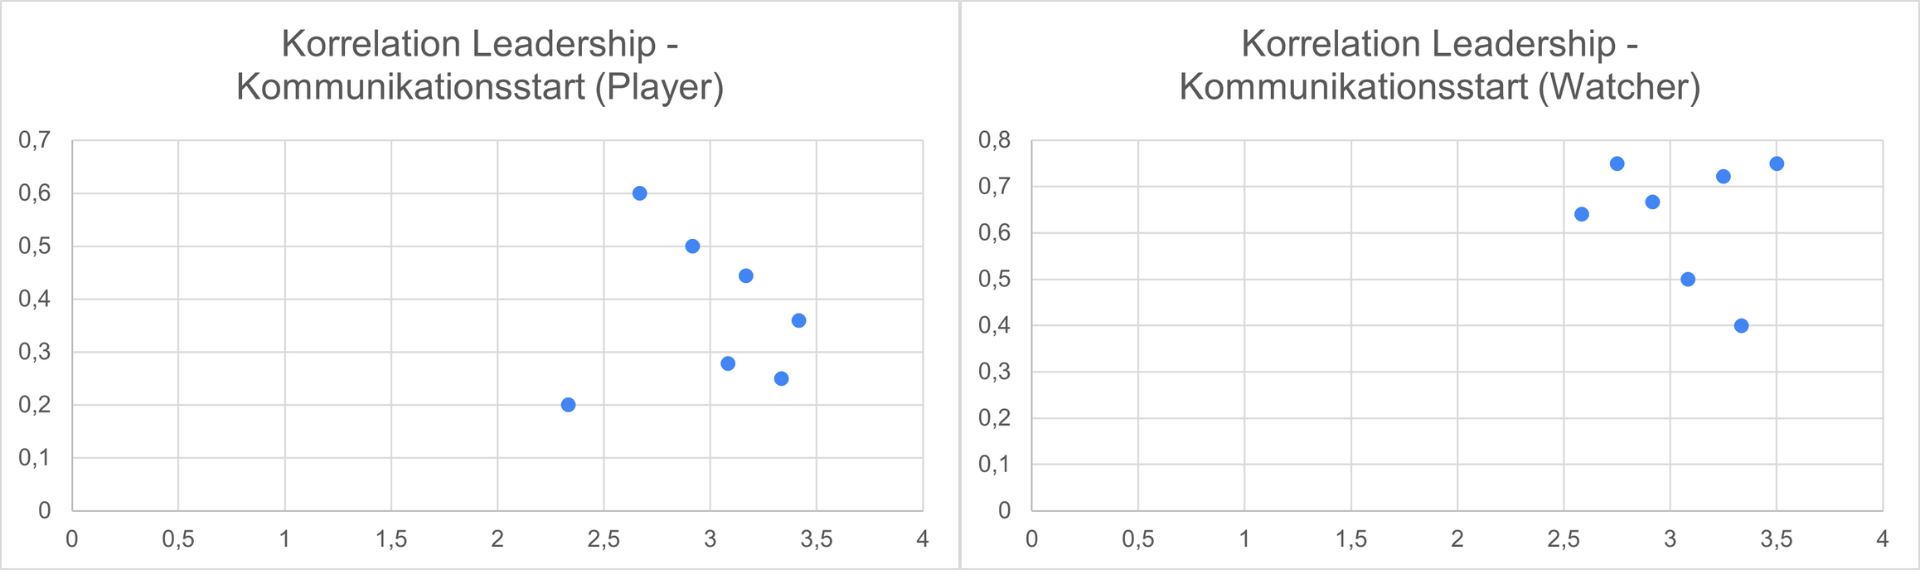
\includegraphics[width=1\linewidth]{content/pictures/Korrelation_Leaderhip_Start_of_conversation.png}
\caption{Korrelation des Leaderships von Player und Watchern mit dem Anteil der Konversationsstarts}
\label{fig:correlation_leadership_conversation_starts}
\end{figure}

Insgesamt zeigt sich, dass das mittlere empfundene Leadership keine Auswirkung auf die Entwicklungen innerhalb der quantitativen Untersuchung hat.

\subsection{Vorstellung der Ergebnisse zum Thema Kognitive Empathie}
In diesem Unterkapitel wird das Ergebnis des Fragebogens zur Kognitiven und Affektiven Empathie vorgestellt (Skala von 1 = Stimme überhaupt nicht zu bis 5 = Stimme voll und ganz zu). Hierbei wurden die Einzelwertungen der beiden Fragebögen zur Kognitiven Empathie ausgezählt und zusammengerechnet. Das Gesamtergebnis zeigt, dass die Probanden ein hohes Maß an kognitiver Empathie zeigen (M = 70; SD = 10.21; Maximal Wert 95). 

Ein ungepaarter t-Test-Vergleich bei ungleichen Varianzen zwischen den Probanden der Player (M = 68.71; SD = 9.96) und Watcher (M = 71.29; SD = 11.09) Untergruppe konnte kein signifikanter Unterschied festgestellt werden, obwohl die Wertung der Watcher leicht höher ist, als die der Player. 

Über den Spearman'sche Rangkorrelationskoeffizienten wurde überprüft, ob das hohe Maß an kognitiver Empathie einen Einfluss auf den hohen Anteil an \ac{CF} im Nachtest hat. 

\begin{figure}[ht]
\centering
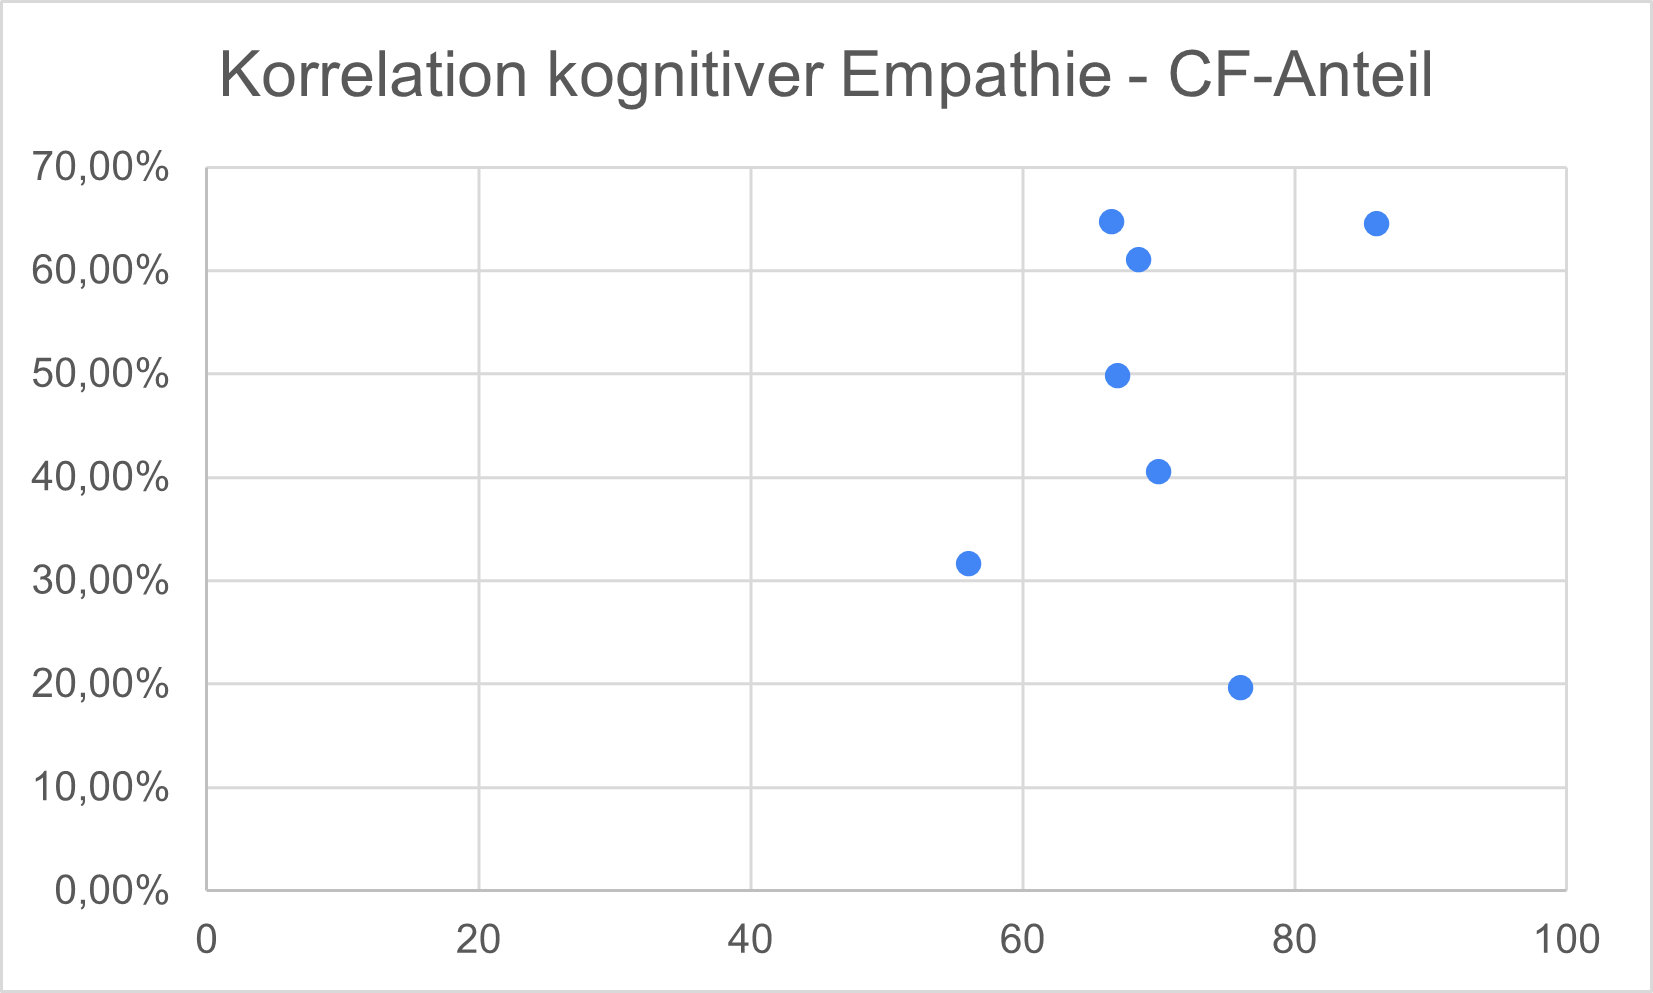
\includegraphics[width=1\linewidth]{content/pictures/Korrelation_Kognitive_Empathie_cfh.png}
\caption{Korrelation kognitiver Empathie mit \ac{CF}-Anteil pro Probanden-Paar}
\label{fig:correlation_kognitive_empathy_cfh}
\end{figure}

Es besteht keine Korrelation (vgl. Abbildung \ref{fig:correlation_kognitive_empathy_cfh}) zwischen der Kognitiven Empathie und dem \ac{CF}-Anteil des Nachtests ((rs(7) = -0.04; p = 0.94).



\subsection{Vorstellung der Ergebnisse zum Thema Fragen zum Nutzen eines spielerischen Ansatzes und Verbesserung der Kommunikation, insbesondere auch im Umgang mit nicht bekannten Personen}

Abschließend werden nun die Ergebnisse vom letzten Fragebogen zum Thema \say{Fragen zum Nutzen eines spielerischen Ansatzes und Verbesserung der Kommunikation, insbesondere auch im Umgang mit nicht bekannten Personen} vorgestellt. Für dieses Thema existiert bislang kein standardisierter Fragebogen. Der für dieses Thema entworfene Fragebogen (Wertung von 1 = Stimme überhaupt nicht zu bis 5 = Stimme voll und ganz zu) umfasst folgende Fragen:
\begin{enumerate}
    \item Spielerische Elemente erleichtern es mir, mit anderen Personen in Kontakt zu treten.
    \item Der Einsatz von Spielelementen (z. B. Aufgaben, Belohnungen, Avatare) kann die Kommunikation zwischen unbekannten Personen fördern.
    \item Ich bin offen dafür, neue Menschen kennenzulernen.
    \item Interaktive oder spielerische Funktionen in digitalen Anwendungen erleichtern mir den Austausch mit anderen.
    \item Ich würde eine digitale Plattform nutzen, die durch spielerische Elemente den Kontakt zu mir unbekannten Personen erleichtert.
    \item Es fällt mir leichter, mit anderen Personen in Kontakt zu treten, wenn spielerische Komponenten involviert sind.
    \item Ich erkenne einen Mehrwert darin, spielerische Kommunikation in beruflichen oder sozialen Kontexten zu integrieren.
\end{enumerate}

Die Fragen 1,2,4 und 6 können dabei in die Kategorie \say{Gamification erleichtert soziale Interaktion} eingeteilt werden. Die Frage 5 umfasst die Kategorie \say{Akzeptanz / Nutzungsintention gamifizierter Plattformen}. Die Fragen 3 und 7 bilden die Kategorie der \say{sozialen Offenheit und Haltung zu spielerischer Kommunikation}.

Beim Thema \say{Gamifikation erleichtert soziale Interaktion} zeigen die Ergebnisse der Probanden ein hohes Maß an Zustimmung (M = 4.42: SD = 0.61). Zum Thema \say{Akzeptanz / Nutzungsintention gamifizierter Plattformen} zeigt sich ein eher wechselhaftes Gesamtbild (M = 3.5; SD = 1.27). Allerdings zeigen sie eher eine soziale Offenheit und Haltung gegenüber spielerischer Kommunikation (M = 3.77; SD = 0.95).

\section{Hypothesenüberprüfung}
Aufgrund des Umfangs des Forschungshintergrundes und des Versuchsaufbaus wurden im Vorfeld der Nutzerstudie die Anzahl der zu überprüfenden Hypothesen auf fünf festgelegt.

Wie im Kapitel der Analysen der artverwandten Spielen, wurden zunächst Hypothesen, die vor der Durchführung der Nutzerstudie formuliert wurden, mit den dokumentierten Ergebnissen verglichen. 

Die Ergebnisse der ausgewerteten Fragebögen und Transkripte zeigen, dass mit Connecting-Minds ein spannendes Spiel konzipiert und umgesetzt werden konnte, das durch seine Spielmechanik eine interessante Erfahrung bieten konnte. Allerdings konnte keine gute gebrauchstaugliche Steuerung in die Anwendungen eingebaut werden, wodurch das Spielerlebnis und die Wirkung des Prototyps gemindert wurde. Allerdings konnte beobachtet und festgestellt werden, dass die soziale Nähe der Probanden gestiegen ist und der Prototyp auf diese eine Auswirkung hat. Aufgrund der niedrigen Teilnehmerzahl der Nutzerstudie konnten keine signifikanten Veränderungen im Kommunikationsverhalten festgestellt werden, wodurch die Kernwirkung des Prototyps nicht bestätigt werden konnte. Jedoch kann die Anwendung dazu beitragen, dass die Hemmschwelle für das Kennenlernen von für sich fremden Personen sinkt.

\begin{figure}[ht]
\centering
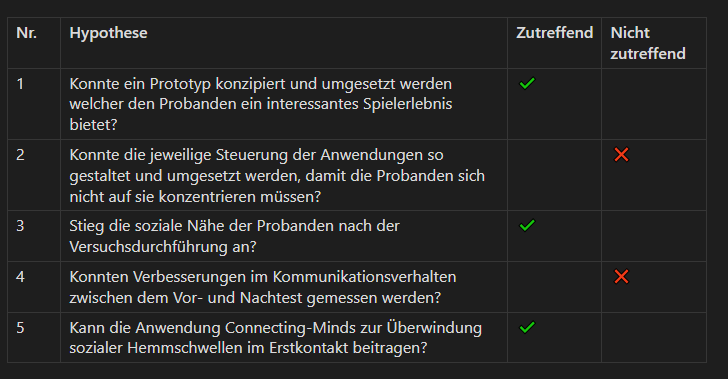
\includegraphics[width=1\linewidth]{content/pictures/Hypothesen_Nutzerstudie.PNG}
\caption{Hypothesenüberprüfung der Nutzerstudie}
\label{fig:hypothesis_user_study}
\end{figure}

\section{Handlungsempfehlungen}
q

\section{Zusammenfassung und Interpretation der Ergebnisse}

\section{Methodendiskussion}
\chapter{Fazit}

\chapter{Diskussion}
\chapter{Ausblick} 


% Schalgwortverzeichnis (Index)
%\printindex

% Literaturverzeichnis
\singlespacing
\bibliographystyle{agsm}
\bibliography{references}

% Eidesstattliche Erklärung
\chapter*{Versicherung über redliches wissenschaftliches Arbeiten\markboth{Versicherung über redliches wissenschaftliches Arbeiten}{}}
% Eintrag in das Inhaltsverzeichnis 
\addcontentsline{toc}{chapter}{Versicherung über redliches wissenschaftliches Arbeiten}

Hiermit versichere ich, Nick Philipp Häcker, dass ich die vorliegende Arbeit selbstständig verfasst und erstellt habe. Ich versichere, dass ich nur zugelassene Hilfsmittel und keine anderen als die angegebenen Quellen und Hilfsmittel benutzt habe. Ferner versichere ich, dass ich alle wörtlich oder sinngemäß übernommenen Stellen in der Arbeit gemäß gängiger wissenschaftlicher Zitierregeln korrekt zitiert und als solche gekennzeichnet habe. Darüber hinaus versichere ich, dass alle verwendeten Hilfsmittel, wie KI-basierte Chatbots (bspw. ChatGPT), Übersetzungs- (bspw. Deepl), Paraphrasier- (bspw. Quillbot) oder Programmier-Applikationen (bspw. Github Copilot) vollumfänglich deklariert und ihre Verwendung an den entsprechenden Stellen angegeben und gekennzeichnet habe.\newline

Ich bin mir bewusst, dass die Nutzung maschinell generierter Texte keine Garantie für die Qualität von Inhalten und Text gewährleistet. Ich versichere, dass ich mich textgenerierender KI-Tools lediglich als Hilfsmittel bedient habe und in der vorliegenden Arbeit mein gestalterischer Einfluss überwiegt. Ich verantworte die Übernahme jeglicher von mir verwendeter maschinell generierter Textpassagen vollumfänglich selbst. \newline

Auch versichere ich, die „Satzung der Hochschule Furtwangen (HFU) zur Sicherung guter wissenschaftlicher Praxis“ vom 27. Oktober 2022 zur Kenntnis genommen zu haben und mich an den dortigen Ausführungen zu orientieren.
Mir ist bewusst, dass meine Arbeit auf die Benutzung nicht zugelassener Hilfsmittel oder Plagiate überprüft werden kann. Auch habe ich zur Kenntnis genommen, dass ein Verstoß gegen § 10 bzw. § 11 Absatz 4 und 5 der Allgemeinen Teile der HFU-SPOen zu einer Bewertung der betroffenen Arbeit mit der Note 5 oder mit «nicht ausreichend» und/oder zum Ausschluss von der Erbringung aller weiteren Prüfungsleistungen führen kann.


Ort, Datum		  \hspace{5cm}                  Unterschrift


\vspace*{1.5cm} \par
\line(1,0){200} \par
\docOrt, \docAbgabedatum ~~\docVorname~\docNachname


%Zurücksetzen \chaptermark
\let\chaptermark\oldchaptermark

% Hier können Anhaenge angefuegt werden
\begin{appendices}
% \chapter{Monatsberichte}
% Nun folgen die Monatsberichte
\newpage
% % \appendixsection{Monatsbericht Februar}Thesis Präsentation als PDF}{content/attachments/Praesentation.pdf}
% \includepdf[pages=-]{content/attachments/reportPraesentation.pdf}
% \appendixsection{Monatsbericht Januar}{content/attachments/report.pdfGamedesign Dokument Gamedesign Workshop}{content/attachments/gdd.pdf}
% \includepdf[pages=-]{content/attachments/gdd}
\end{appendices}
\end{document}      